\newcommand{\ttbar}{$\textrm{t}\bar{\textrm{t}}~$}
\newcommand{\bbbar}{$\textrm{b}\bar{\textrm{b}}~$}
\newcommand{\ptmiss}{$p_{T}^{\mathrm{miss}}~$}

\chapter{Search for physics beyond the Standard Model using boosted H bosons and missing transverse momentum in proton-proton collisions at 13 TeV}
\label{chap:analysis}

\section{Motivation \& Strategy}

If a more unifying theory than the SM exists it certainly has not been forthright in its manifestation. One possibility for the lack of discoveries of phenomena not explained within the SM is that there are indeed particles existing in Nature which have not been observed, but they have such a large mass the energy of the proton-proton collisions provided by the LHC is insufficient to directly create them. The outcome of many searches for new particles is thus the setting of lower limits placed on the mass -- if the particle were any lighter than this limit it would have been produced copiously enough for its unambiguous detection (see for example \cite{CMS-SUS-16-033}, \cite{CMS-SUS-15-002}). As these particles become more massive more momentum is imparted upon the particles involved in the final state; any SM particles resulting from the decay of higher mass states will be produced with large momentum (this is called high boost). As a particle becomes more boosted its decay products are emitted at smaller angles, eventually collimating sufficiently to be reconstructed as a single jet. If new physics exists with masses achievable by the LHC, one could suspect that there exists non-zero coupling with the electroweak H, Z, or W bosons. Observation of events containing high-$p_{T}$ ($>$300 GeV) electroweak bosons are thus of considerable interest for some hints of something unseen.

The Minimal Supersymmetric SM contains a $\mathbb{Z}_{2}$ symmetry in which all SM particles have charge -1 and all supersymmetric particles have charge +1, this is called R-parity\cite{susyprimer}. One direct consequence of R-parity is that the decay of a massive supersymmetric particle must include at least one supersymmetric particle in the final state. Necessarily this is the lightest such particle in the theory, denoted the lightest supersymmetric particle (LSP). If the LSP is electrically neutral it may escape detection, creating an imbalance in the net momentum of the event (as would a neutrino). Events with a large momentum imbalance are also interesting as potential regions for SUSY.

With this as motivation, we designed an analysis searching for hints of new physics beyond the SM in events with boosted H or Z bosons and a large transverse momentum imbalance of the event. We reconstruct the H and Z bosons in the $b\bar{b}$ channel, with 57\% and 15\% branching fractions respectively. Although our analysis is sensitive to any new physics with this final state, we have adopted two benchmark models (known as SMS models\cite{CMS-SUS-11-016}, which are phenomenological models of SUSY production), seen in Figure \ref{fig:sms}, to give motivation to the analysis. In this scenario, the proton-proton interaction produces a pair of gluinos $\tilde{g}$ which decay to a neutralino $\tilde{\chi}_{2}^{0}$ by the emission of SM quarks. A small mass splitting between the gluino $\tilde{g}$ and neutralino $\tilde{\chi}_{2}^{0}$ will result in low-$p_{T}$ SM quarks and a high-$p_{T}$ neutralino $\tilde{\chi}_{2}^{0}$. This neutralino $\tilde{\chi}_{2}^{0}$ further decays into neutralino $\tilde{\chi}_{1}^{0}$ with the emission of a H or Z boson. The neutralino $\tilde{\chi}_{1}^{0}$ is the LSP and escapes detection. 
 
Past searches targeting similar final states (but different production scenario, i.e. another SMS model) have been performed in which the H bosons are produced with low-$p_{T}$, in this case the H bosons are reconstructed as a resolved pair of b-tagged AK4 jets \cite{CMS-SUS-16-044}.
 
\begin{figure}
\centering
\begin{subfigure}[b]{0.45\textwidth}
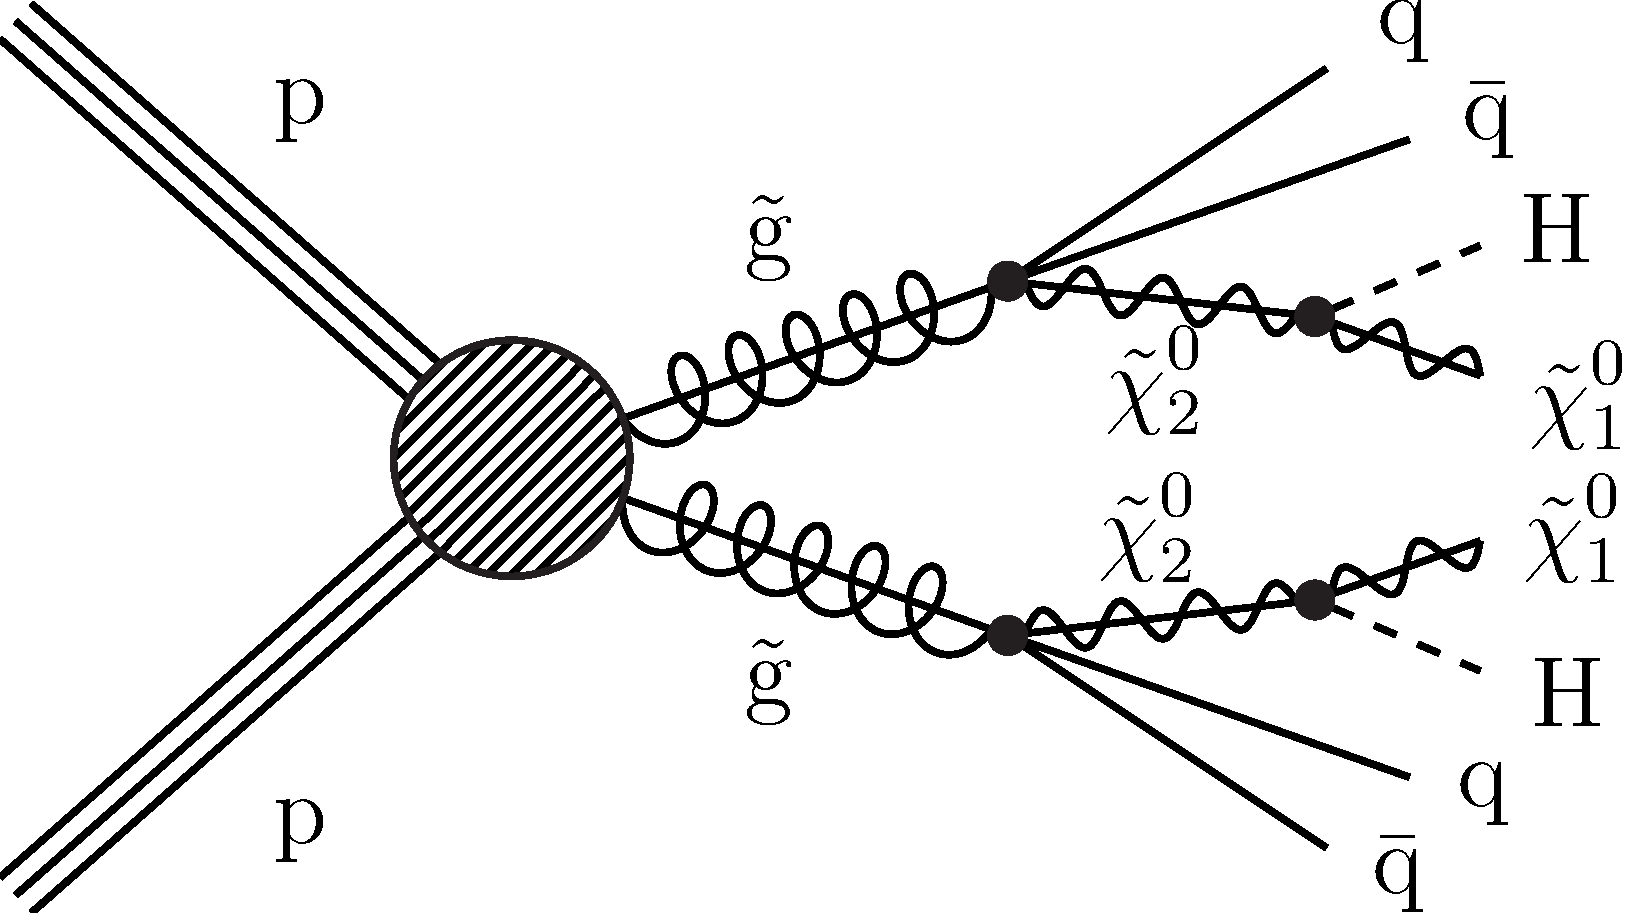
\includegraphics[width=\textwidth]{figs/SUS17006/CMS-SUS-17-006_Figure_001.pdf}
\caption{The T5HH model.}
\label{fig:t5hh}
\end{subfigure}
\begin{subfigure}[b]{0.45\textwidth}
\centering
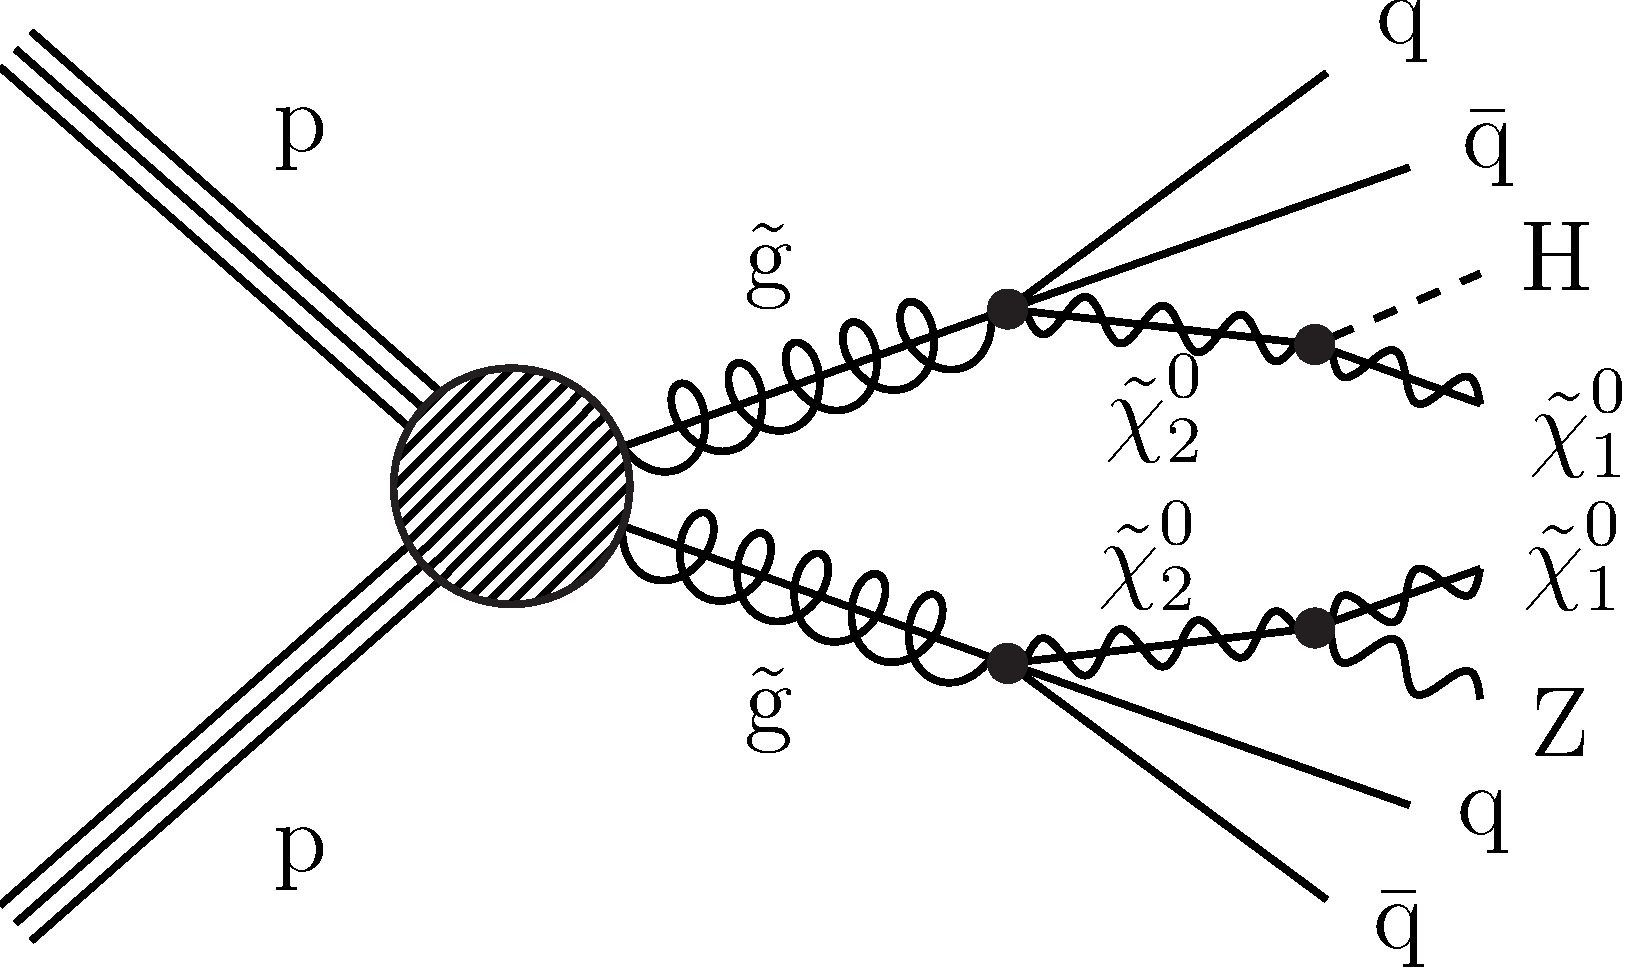
\includegraphics[width=\textwidth]{figs/SUS17006/CMS-SUS-17-006_Figure-aux_001.pdf}
\caption{The T5ZH model.}
\end{subfigure}
\caption{Diagrams of the benchmark models used for motivation of the targeted signal.}
\label{fig:sms}
\end{figure}

\section{Object Definition \& Event Selection}

We establish a baseline selection choosing events with all-hadronic final states and missing transverse momentum (\ptmiss), as motivated by Figure \ref{fig:sms}. The baseline selection is as follows:

\begin{itemize}
\item $\geq2$ AK8 jets; $p_{T} > 300\,\mathrm{GeV}$ and $50 < \mathrm{mass} < 250\,\mathrm{GeV}$
\item $p_{T}^{\mathrm{miss}} > 300\,\mathrm{GeV}$; $p_{T}^{\mathrm{miss}} \equiv |-\sum_{\mathrm{PFcandidates}}\vec{p_{T, i}}|$
\item isolated electron veto; $p_{T}>10\,\mathrm{GeV}$\newline
To remove events with top or W production in which the W decays to an electron.
\item isolated muon veto; $p_{T}>10\,\mathrm{GeV}$\newline
To remove events with top or W production in which the W decays to a muon.
\item isolated track veto\newline
To remove events with top or W production in which the W decays to a tau. The tau branching fraction to states containing at least one charged particle is 85\%. As an isolated track is defined by looser criteria than that of an electron or muon, this cut also serves to increase the efficiency of the isolated electron and muon vetoes.

\item $\Delta\phi_{1, 2, 3, 4} > 0.5, 0.5, 0.3, 0.3$; $\Delta\phi_{i}\equiv \Delta\phi(\vec{p_{T}}^{\mathrm{miss}}, \mathrm{AK4\,jet}_{i})$\newline
The $\Delta\phi$ cut is designed to mitigate QCD events in which a jet is under-measured leading to an artificial imbalance in the event momentum. This cut requires that the difference in $\phi$ between the \ptmiss vector and each of the four leading AK4 jets is sufficiently large to remove events in which a jet has been under-measured giving rise to fake \ptmiss pointing in the same direction. If less than four AK4 jets are available the additional cuts are removed.
\end{itemize}

A dedicated heavy tagging algorithm is used to identify AK8 jets arising from the decay of two b quarks \cite{bbtagger}. The distribution of the output discriminator for the lead and sub-leading jets are seen in the left and right panels of Figure \ref{fig:ak8bb}, respectively; signal-like events peak towards larger values. To $b\bar{b}$ tag the AK8 jets we choose the loose working-point ($>$0.3) corresponding to a signal efficiency of approximately $80\%$ per AK8 jet (see Section \ref{sec:reinterpretation}). The stacked histogram and solid lines shows the distribution after baseline selection for simulation and two representative signal points, respectively.

Further H/Z tagging of an AK8 jet is accomplished by restricting the jet mass window to [85, 135 GeV] to be consistent with that of the H boson. The distributions of the jet mass are seen in Figure \ref{fig:ak8mass}. The signal shown in the solid line is the T5HH model (i.e. Figure \ref{fig:t5hh}). The same identification criteria are applied to tag an AK8 jet as either an H or Z boson, there is no distinction made.

\begin{figure}
\begin{subfigure}[b]{0.5\textwidth}
\centering
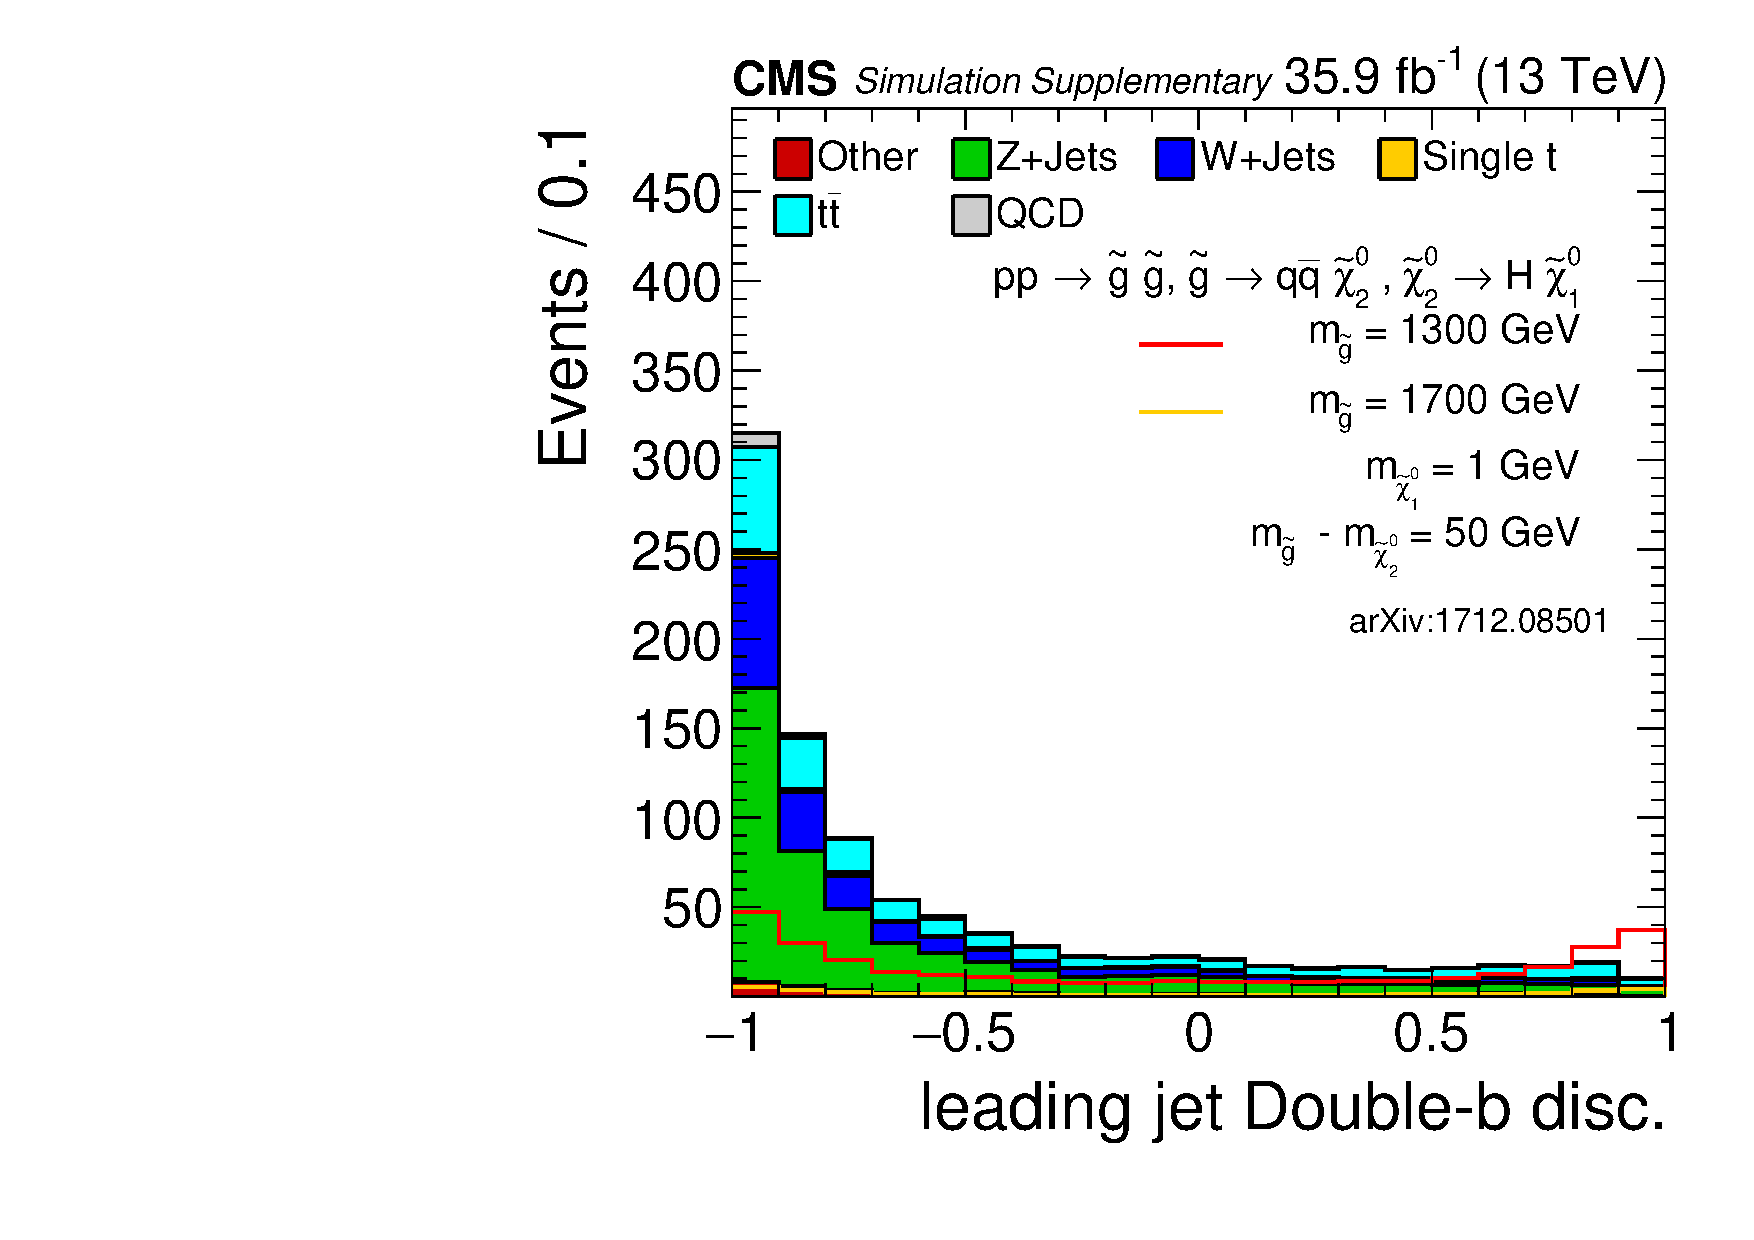
\includegraphics[width=\textwidth]{figs/SUS17006/J1BB_LooseJetMass.pdf}
\end{subfigure}
\begin{subfigure}[b]{0.5\textwidth}
\centering
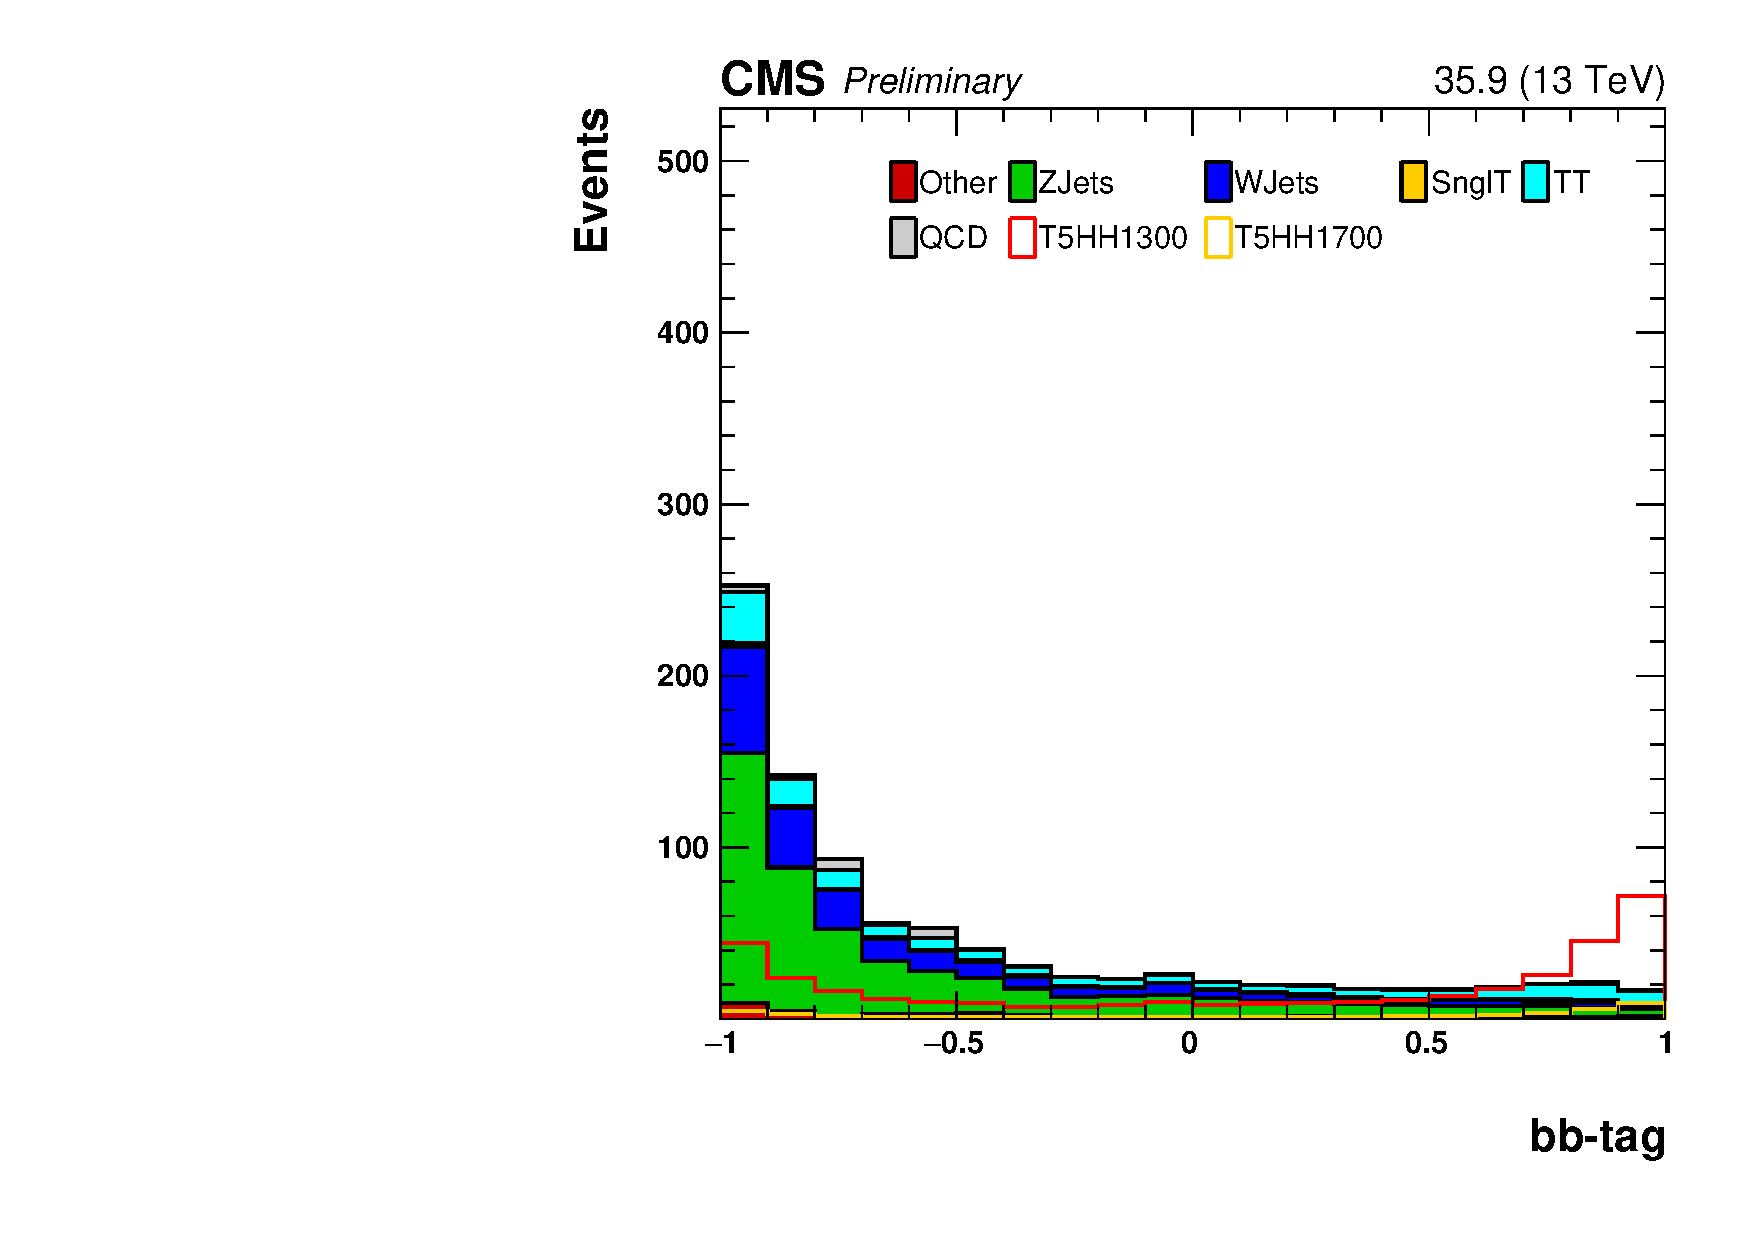
\includegraphics[width=\textwidth]{figs/SUS17006/J2pt_BBtag_baseline.pdf} 
\end{subfigure}
\caption{$b\bar{b}$ tagging neural network discriminator.}
\label{fig:ak8bb}
\end{figure}

\begin{figure}
\begin{subfigure}[b]{0.5\textwidth}
\centering
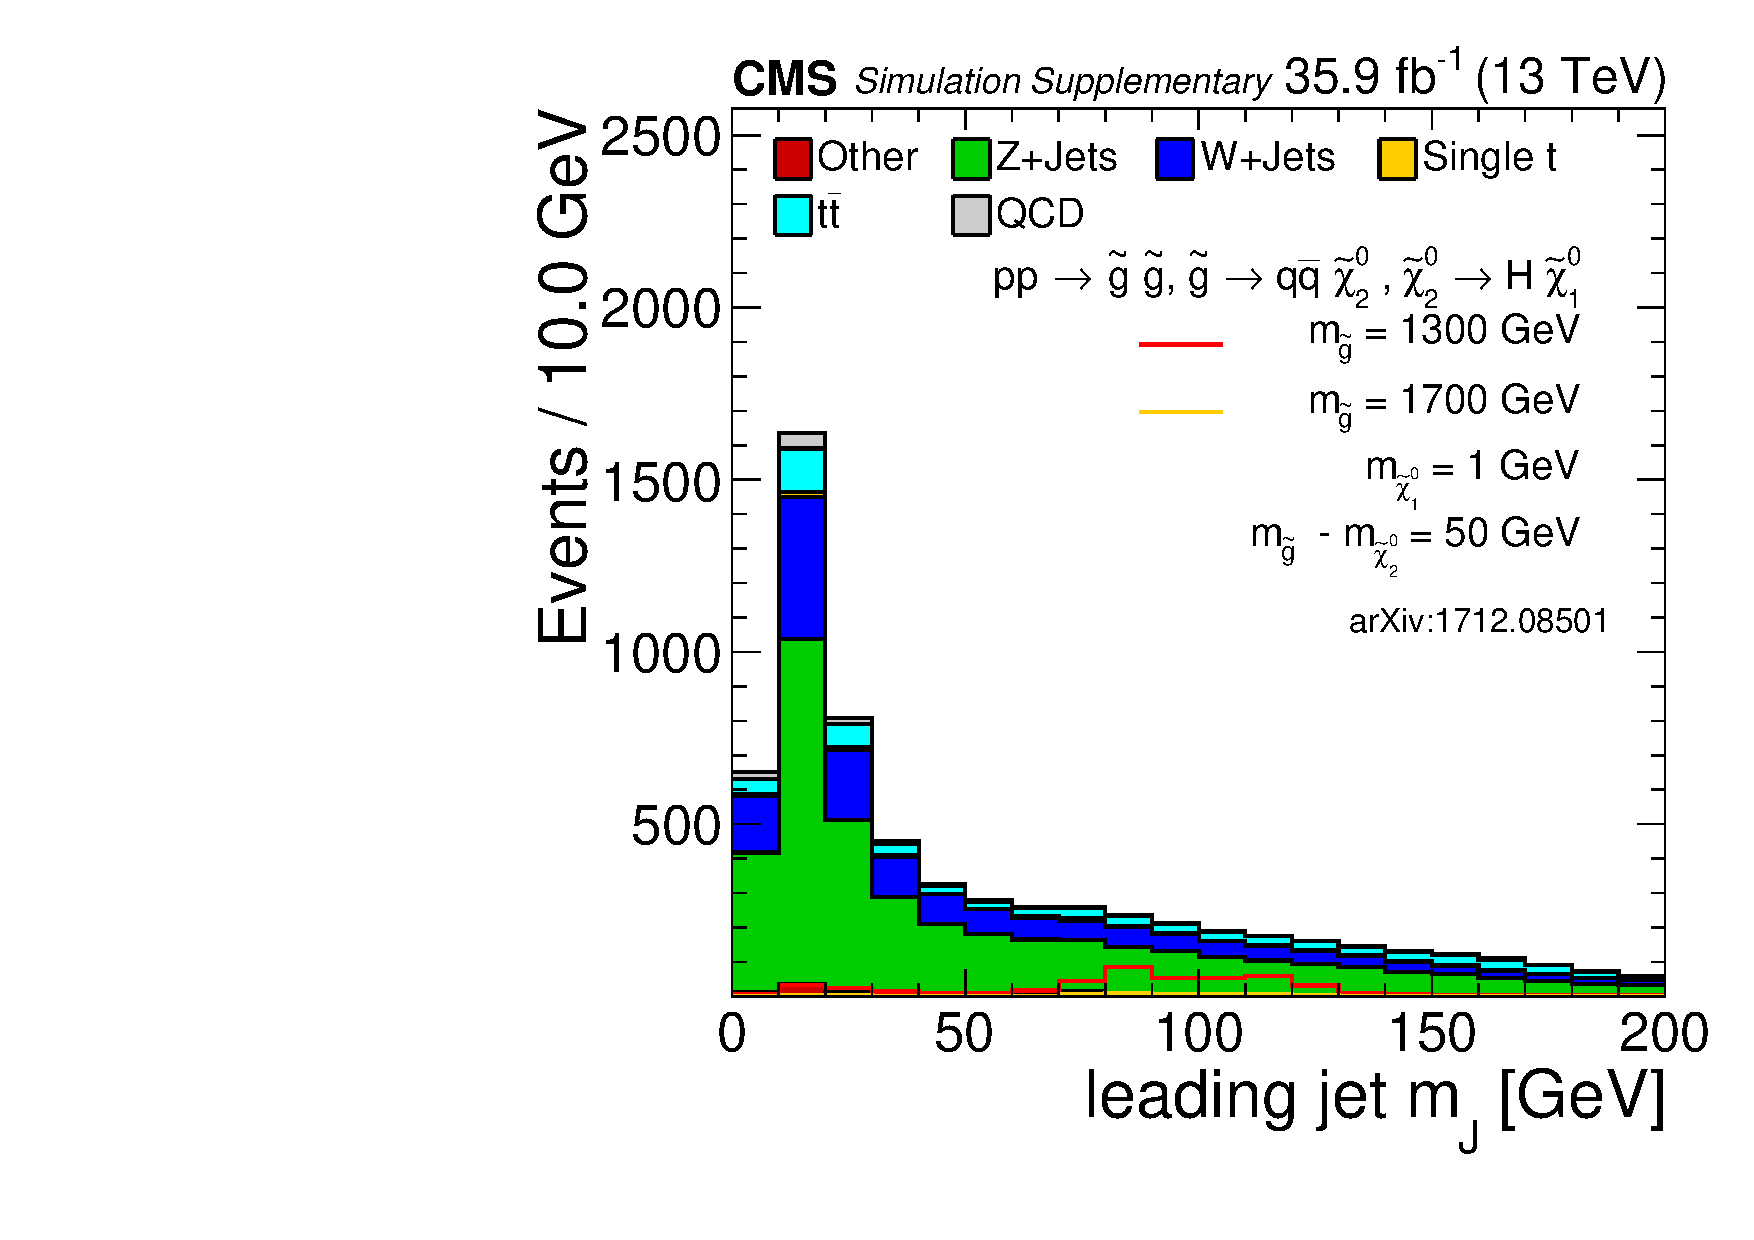
\includegraphics[width=\textwidth]{figs/SUS17006/J1Mwide_JetPt.pdf}
\end{subfigure}
\begin{subfigure}[b]{0.5\textwidth}
\centering
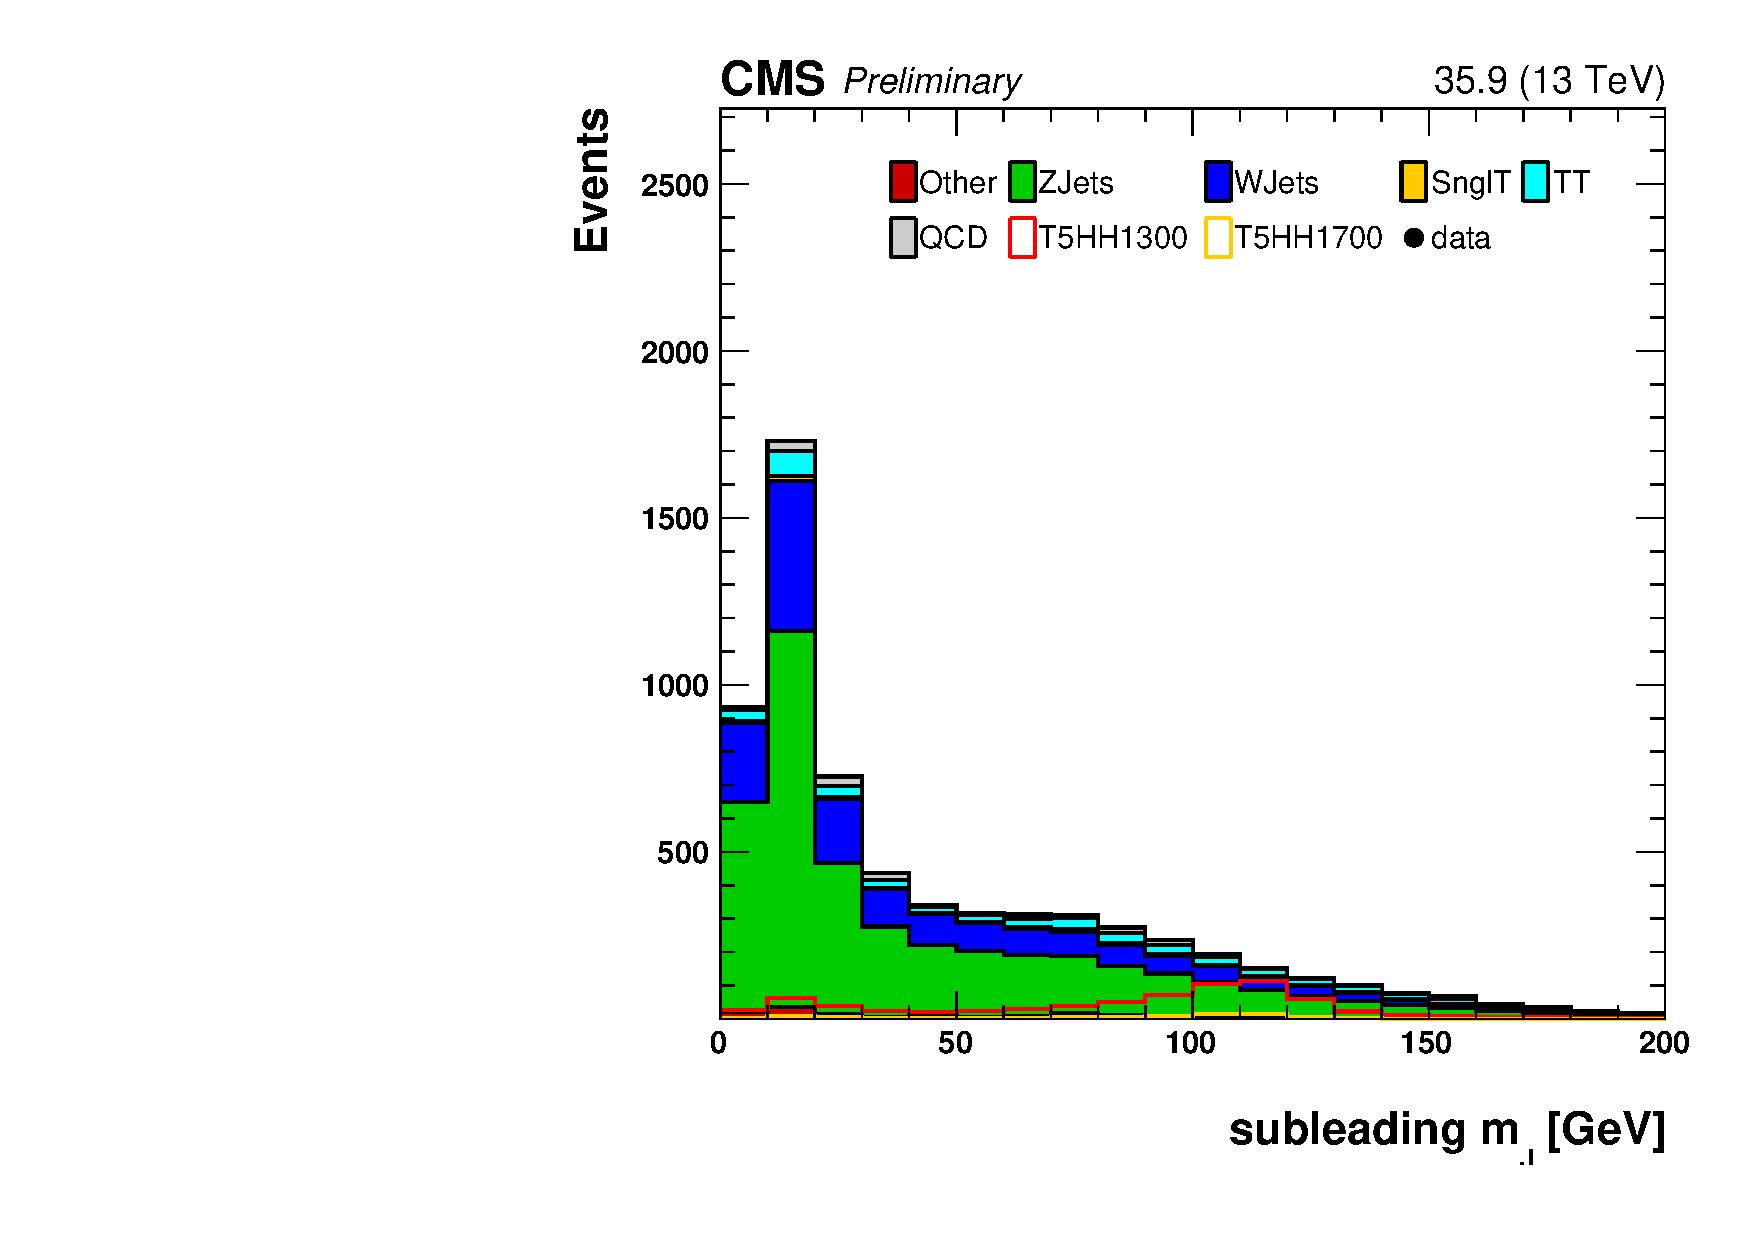
\includegraphics[width=\textwidth]{figs/SUS17006/J2Mwide_JetPt.pdf} 
\end{subfigure}
\caption{The AK8 jet mass.}
\label{fig:ak8mass}
\end{figure}

\section{Dataset and Trigger}

We use a total of 35.9 $\mathrm{fb}^{-1}$ of data collected by the CMS experiment in 2016. Events are selected in data using a trigger which requires greater than 100 GeV of \ptmiss calculated at high-level trigger (HLT); additionally the logical OR of two other triggers with thresholds of 110 and 120 GeV are applied. The trigger efficiency is derived in data using a single-electron reference trigger requiring a tight-ID electron of $p_{T}$$>$27 GeV. We further select events with at least three AK4 jets and exactly one reconstructed electron of $p_{T}$$>$25 GeV. The signal region trigger is found to be greater than 98\% for events with \ptmiss$>$250 GeV and HT$>$300 GeV \cite{CMS-SUS-16-033}.

\section{Event Simulation}

Event simulation of the proton-proton collisions proceeds in a step-wise manner.
To simulate the hard physics process MadGraph@NLO2.2.2 \cite{Alwall:2014hca} is used to calculate matrix-element amplitudes. The parton distribution functions (PDFs) used in these calculations are from NNPDF 3.0 \cite{Ball:2014uwa}.
Parton showering and other event dynamics are generated with Pythia.
The simulation of the interaction of the final state particles with the detector is performed with GEANT \cite{Agostinelli:2002hh}.
This ``raw'' simulation data is then at the same tier as data collected from the physical experiment and is merged into a single pipeline for event reconstruction.

\subsection{Standard Model Processes}

The SM samples which enter as the primary backgrounds are listed in Tables \ref{tab:ttbarMCsamples}, \ref{tab:qcdMCsamples}, \ref{tab:zjetsMCsamples}, and \ref{tab:wjetsMCsamples} (see Section \ref{sec:smbkg} for a discussion of the SM background). All samples are generated with a pileup distribution with an average of 25 interactions per bunch crossing and a 25ns interval between bunches. The MC samples are used to validate the background estimation methods and control regions. For acceptable statistics over a wide range of parameter space, the MC samples are often binned in $\mathrm{HT}\equiv\sum_{AK4\,jets}p_{T}$. As our event selection requires at least two AK8 jets with $p_{T}$$>$300 GeV we roughly operate in regime of HT$>$600 GeV.

\begin{table}
\centering
\caption{SM $t\bar{t}$ MC samples used in the analysis. The cross sections are calculated to NNLO.}
\label{tab:ttbarMCsamples}
\begin{tabular}{cclll}
\hline \hline
process & final state & HT (GeV) & $\sigma$ (pb) & $\int\mathcal{L}$ (fb$^{-1}$)\\
\hline
\ttbar+jets & $t\rightarrow\ell\nu, \bar{t}\rightarrow2q$ & inclusive & 182.72 & 283.90\\
\ttbar+jets & $\bar{t}\rightarrow\ell\nu, t\rightarrow2q$ & inclusive & 182.72 & 326.48\\
\ttbar+jets & $2\ell$    & inclusive & 88.34 & 346.25\\
\ttbar+jets & inclusive & [600, 800] & 2.734 & 5231.81\\
\ttbar+jets & inclusive & [800, 1200] & 1.121 & 9416.61\\
\ttbar+jets & inclusive & [1200, 2500]  & 0.198 & 14819.34\\
\ttbar+jets & inclusive & [2500, $\infty$] & 0.002 & 221088.29\\
\hline \hline
\end{tabular}
\end{table}

\begin{table}
\centering
\caption{SM QCD MC samples used in the analysis. All cross sections are calculated to LO.}
\label{tab:qcdMCsamples}
\begin{tabular}{lllll}
\hline \hline
process & HT (GeV) & $\sigma$ (pb) & $\int\mathcal{L}$ (fb$^{-1}$)\\\hline
QCD & [200, 300] & 1735000 & 0.03\\
QCD & [300, 500] & 366800 & 0.16\\
QCD & [500, 700] & 29370 & 1.95\\
QCD & [700, 1000] & 6524 & 6.68\\
QCD & [1000, 1500] & 1064 & 12.62\\
QCD & [1500, 2000] & 121.5 & 32.63\\
QCD & [2000, $\infty$] & 25.42 & 239.30\\
\hline \hline
\end{tabular}
\end{table}

\begin{table}
\centering
\caption{SM $Z\rightarrow\nu\nu+$jets MC samples used in the analysis. The cross sections are calculated to NNLO.}
\label{tab:zjetsMCsamples}
\begin{tabular}{llll}
\hline \hline
process & HT (GeV) & $\sigma$ (pb) & $\int\mathcal{L}$ (fb$^{-1}$)\\\hline
Z($\rightarrow\nu\bar{\nu}$)+jets & [100, 200] & 344.8 & 54.13\\
Z($\rightarrow\nu\bar{\nu}$)+jets & [200, 400] & 95.53 & 208.46\\
Z($\rightarrow\nu\bar{\nu}$)+jets & [400, 600] & 13.20 & 77.30\\
Z($\rightarrow\nu\bar{\nu}$)+jets & [600, 800] & 3.148 & 1795.26\\
Z($\rightarrow\nu\bar{\nu}$)+jets & [800, 1200] & 1.451 & 1486.09\\
Z($\rightarrow\nu\bar{\nu}$)+jets & [1200, 2500] & 0.355 & 1029.81\\
Z($\rightarrow\nu\bar{\nu}$)+jets & [2500, $\infty$] & 0.0085 & 47498.87\\
\hline \hline
\end{tabular}
\end{table}

\begin{table}
\centering
\caption{SM $W\rightarrow\ell\nu+$jets MC samples used in the analysis. The cross sections are calculated to NNLO.}
\label{tab:wjetsMCsamples}
\begin{tabular}{cclll}
\hline \hline
process & HT (GeV) & $\sigma$ (pb) & $\int\mathcal{L}$ (fb$^{-1}$)\\\hline
W($\rightarrow\ell\nu$)+jets & [100, 200] & 1627.45 & 18.16\\
W($\rightarrow\ell\nu$)+jets & [200, 400] & 435.24 & 45.88\\
W($\rightarrow\ell\nu$)+jets & [400, 600] & 59.18 & 123.64\\
W($\rightarrow\ell\nu$)+jets & [600, 800] & 14.58 & 221.32\\
W($\rightarrow\ell\nu$)+jets & [800, 1200] & 6.66 & 1123.13\\
W($\rightarrow\ell\nu$)+jets & [1200, 2500] & 1.608 & 153.44\\
W($\rightarrow\ell\nu$)+jets & [2500, $\infty$] & 0.039 & 6497.28\\
\hline \hline
\end{tabular}
\end{table}

\subsection{Signal models}
\label{sec:signal-models}

For commissioning of the analysis technique (as well as the limit-setting procedure, see Section \ref{sec:results}) Monte Carlo samples with our final-state signal topology were generated, as in Figure \ref{fig:sms}. The signal sample follows the same processing chain as the SM samples. The mass splitting between the gluino $\tilde{g}$ and neutralino $\tilde{\chi}_{2}^{0}$ is fixed to 50 GeV, resulting in low $p_{T}$ SM quarks produced in the gluino $\tilde{g}$ decays. The mass of the neutralino $\chi^{0}_{1}$ (LSP) is fixed to 1 GeV. We have samples with a range of gluino $\tilde{g}$ masses from 750 to 2200 GeV. The $p_{T}$ distribution for the generated H bosons in these samples is seen in Figure \ref{fig:GenHiggsBoost} for a number of gluino $\tilde{g}$ masses. Additionally the angular separation $\Delta R \equiv \sqrt{\Delta\phi^{2}+\Delta\eta^{2}}$ between the $b\bar{b}$ pair is shown. As the $p_{T}$ of a parent boson increases the $b\bar{b}$ pair from its decay tend to align, allowing complete reconstruction with a single AK8 jet.

\begin{figure}
\centering
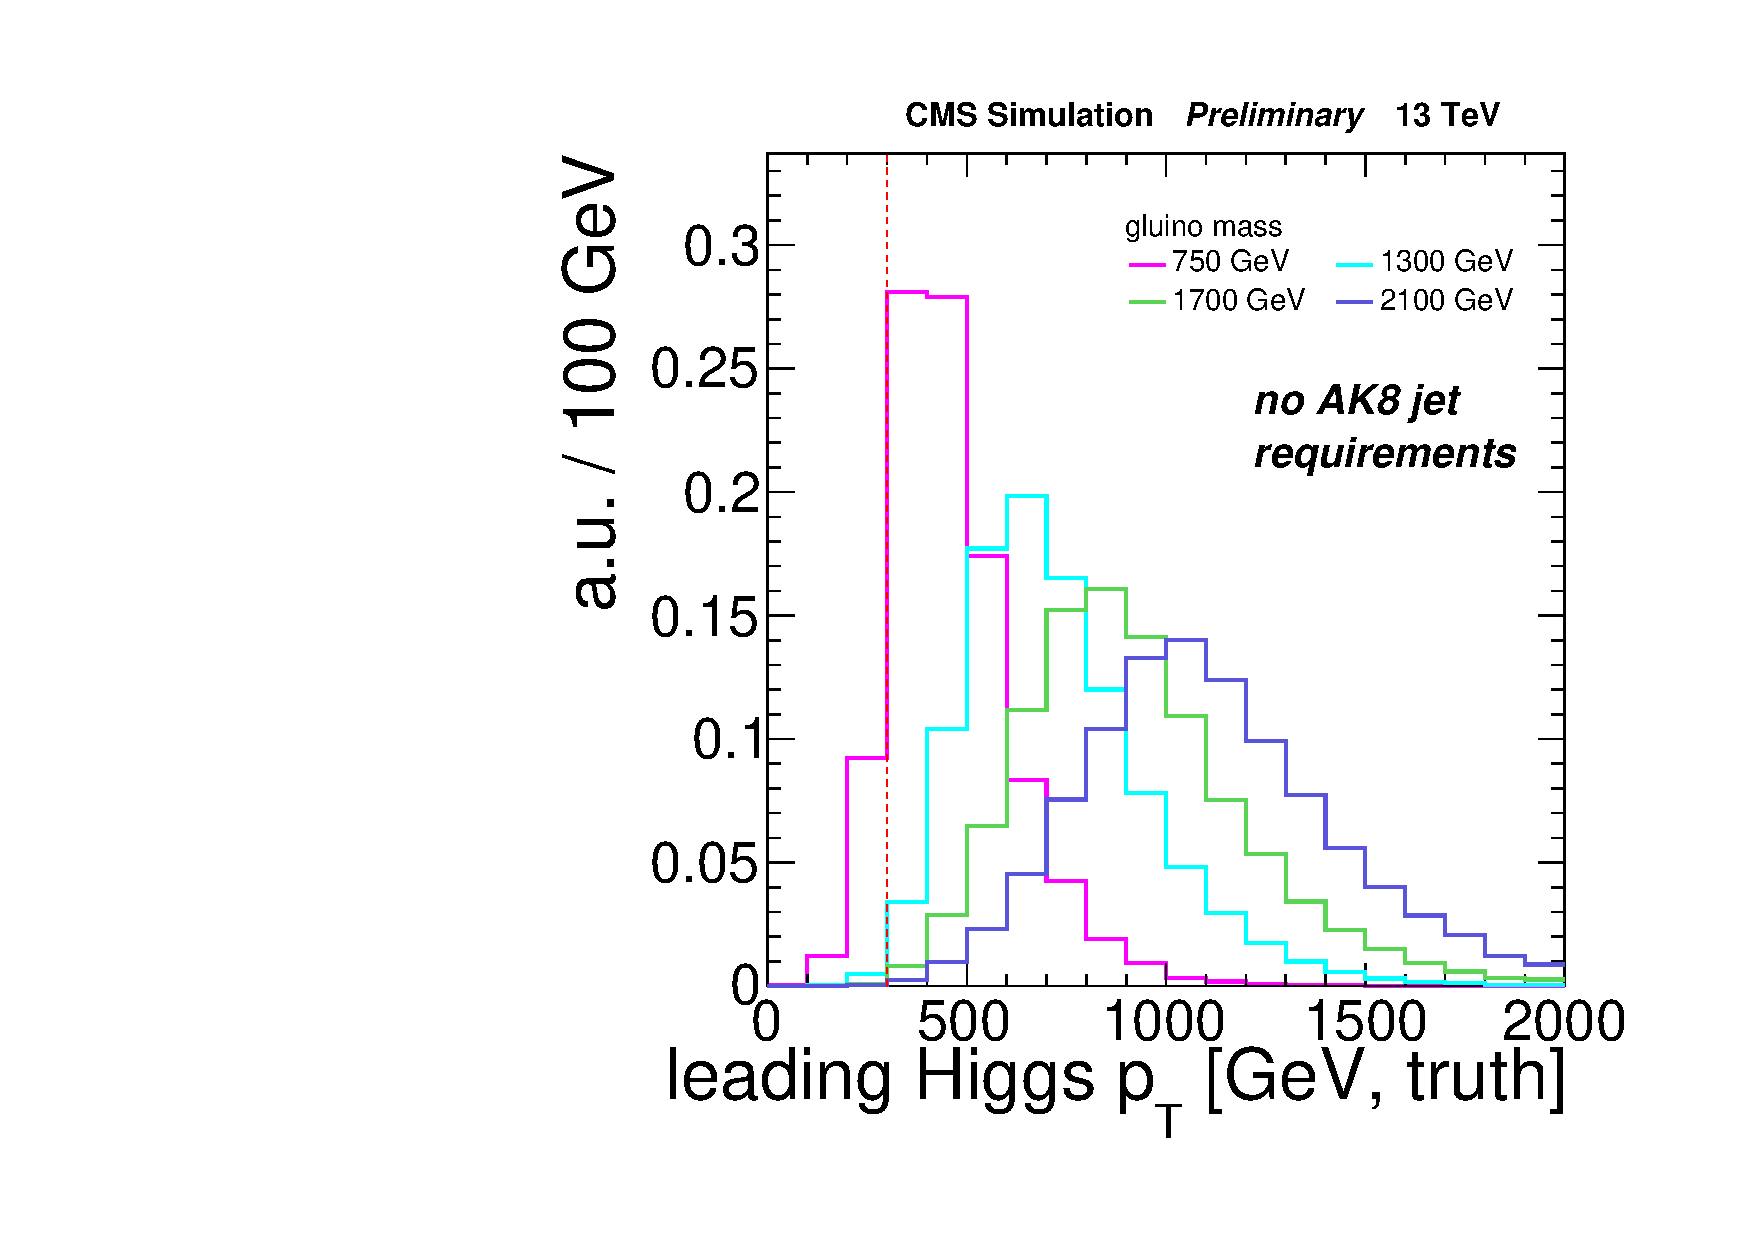
\includegraphics[width=0.45\linewidth]{figs/SUS17006/leadHiggsPt.pdf}
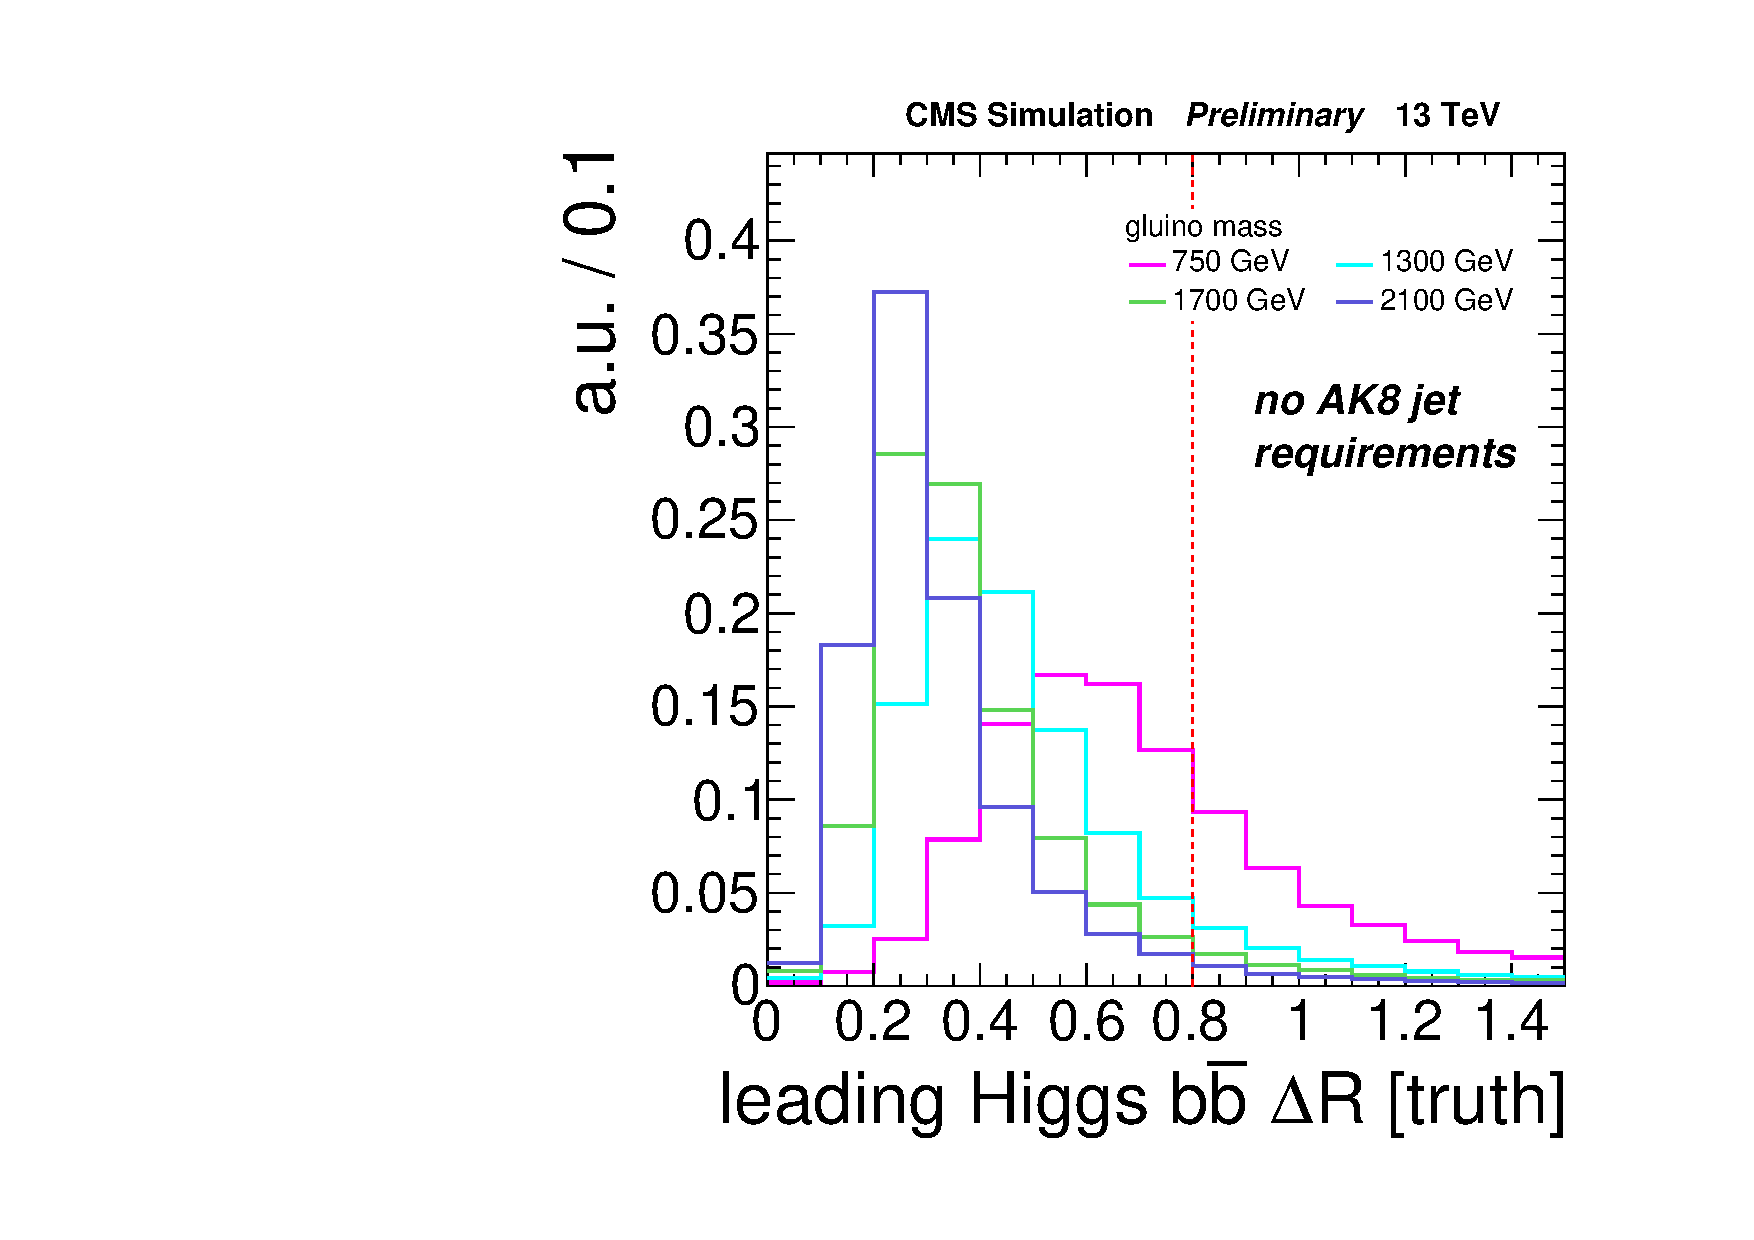
\includegraphics[width=0.45\linewidth]{figs/SUS17006/leadHiggsDr.pdf}\\
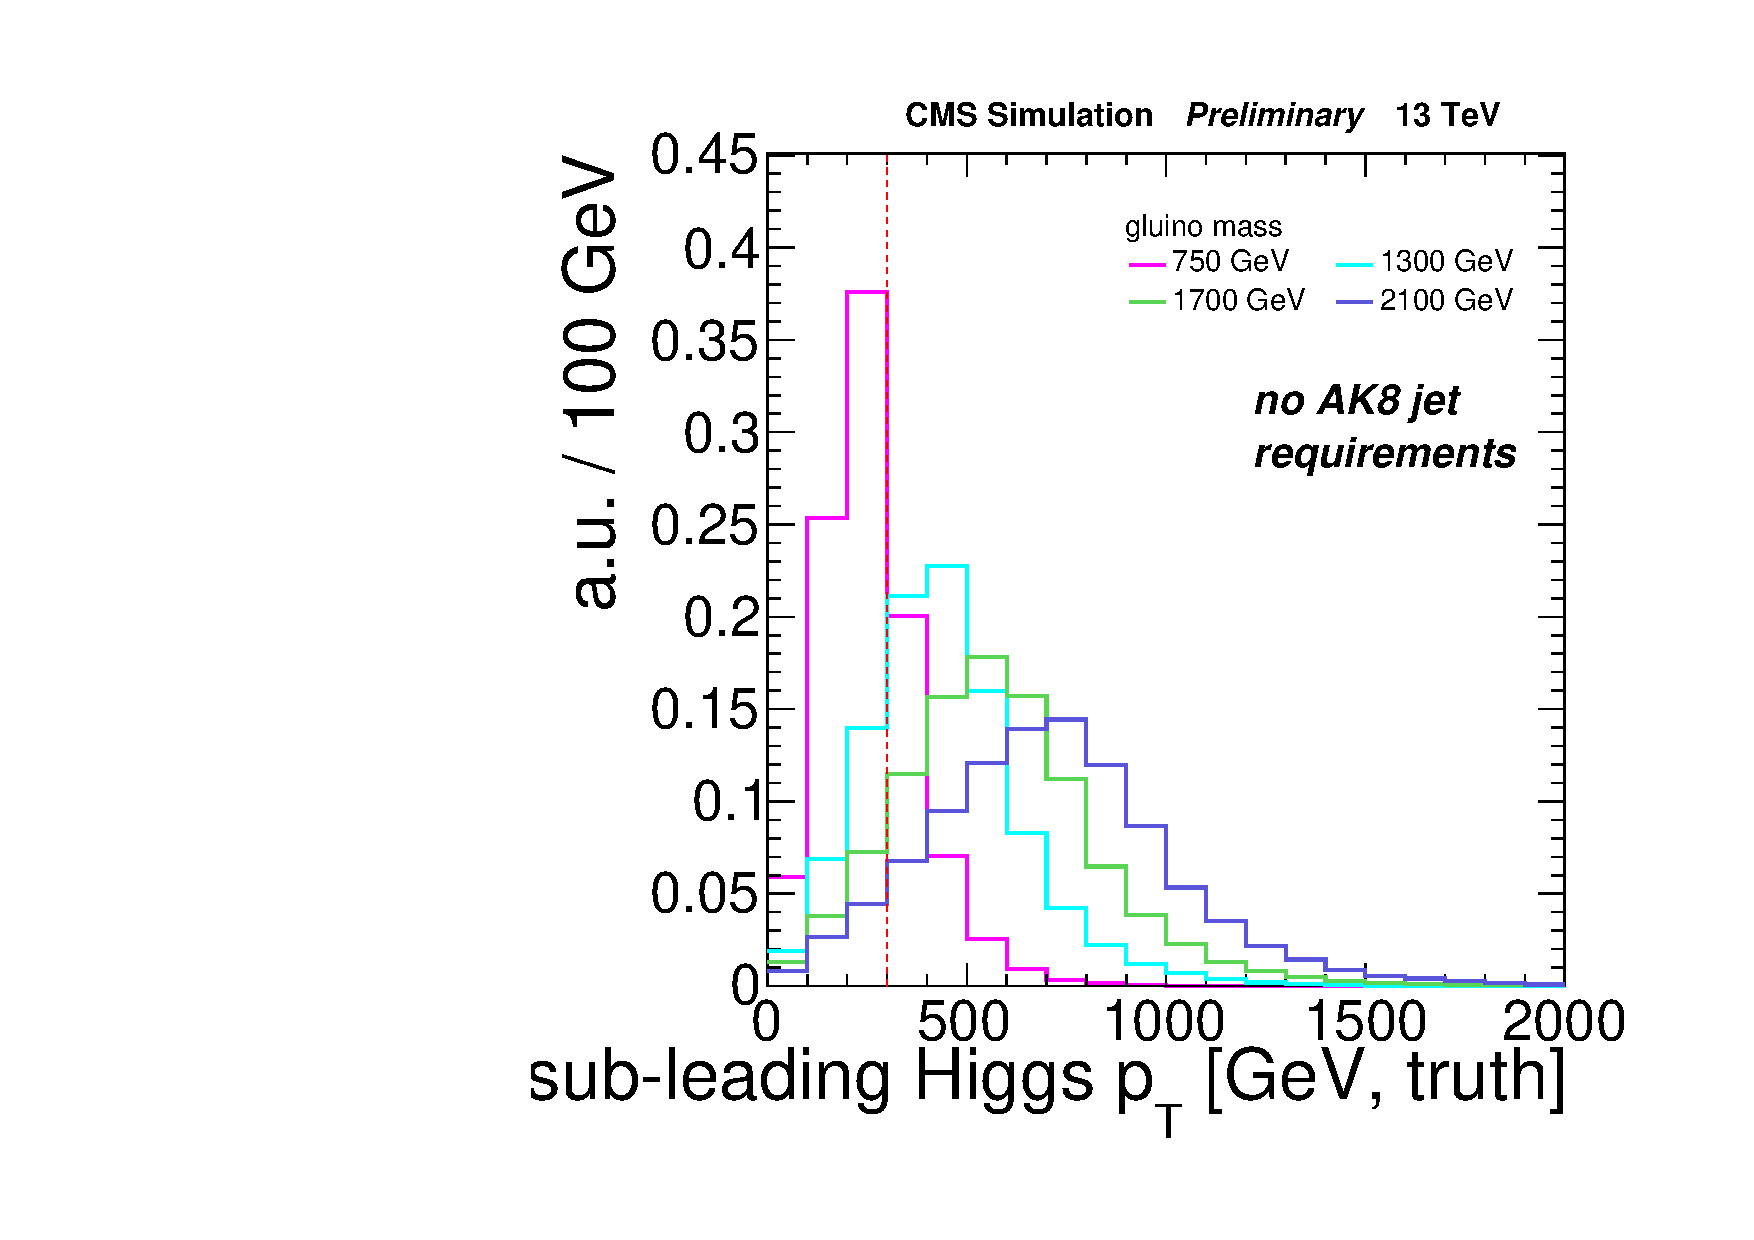
\includegraphics[width=0.45\linewidth]{figs/SUS17006/subleadHiggsPt.pdf}
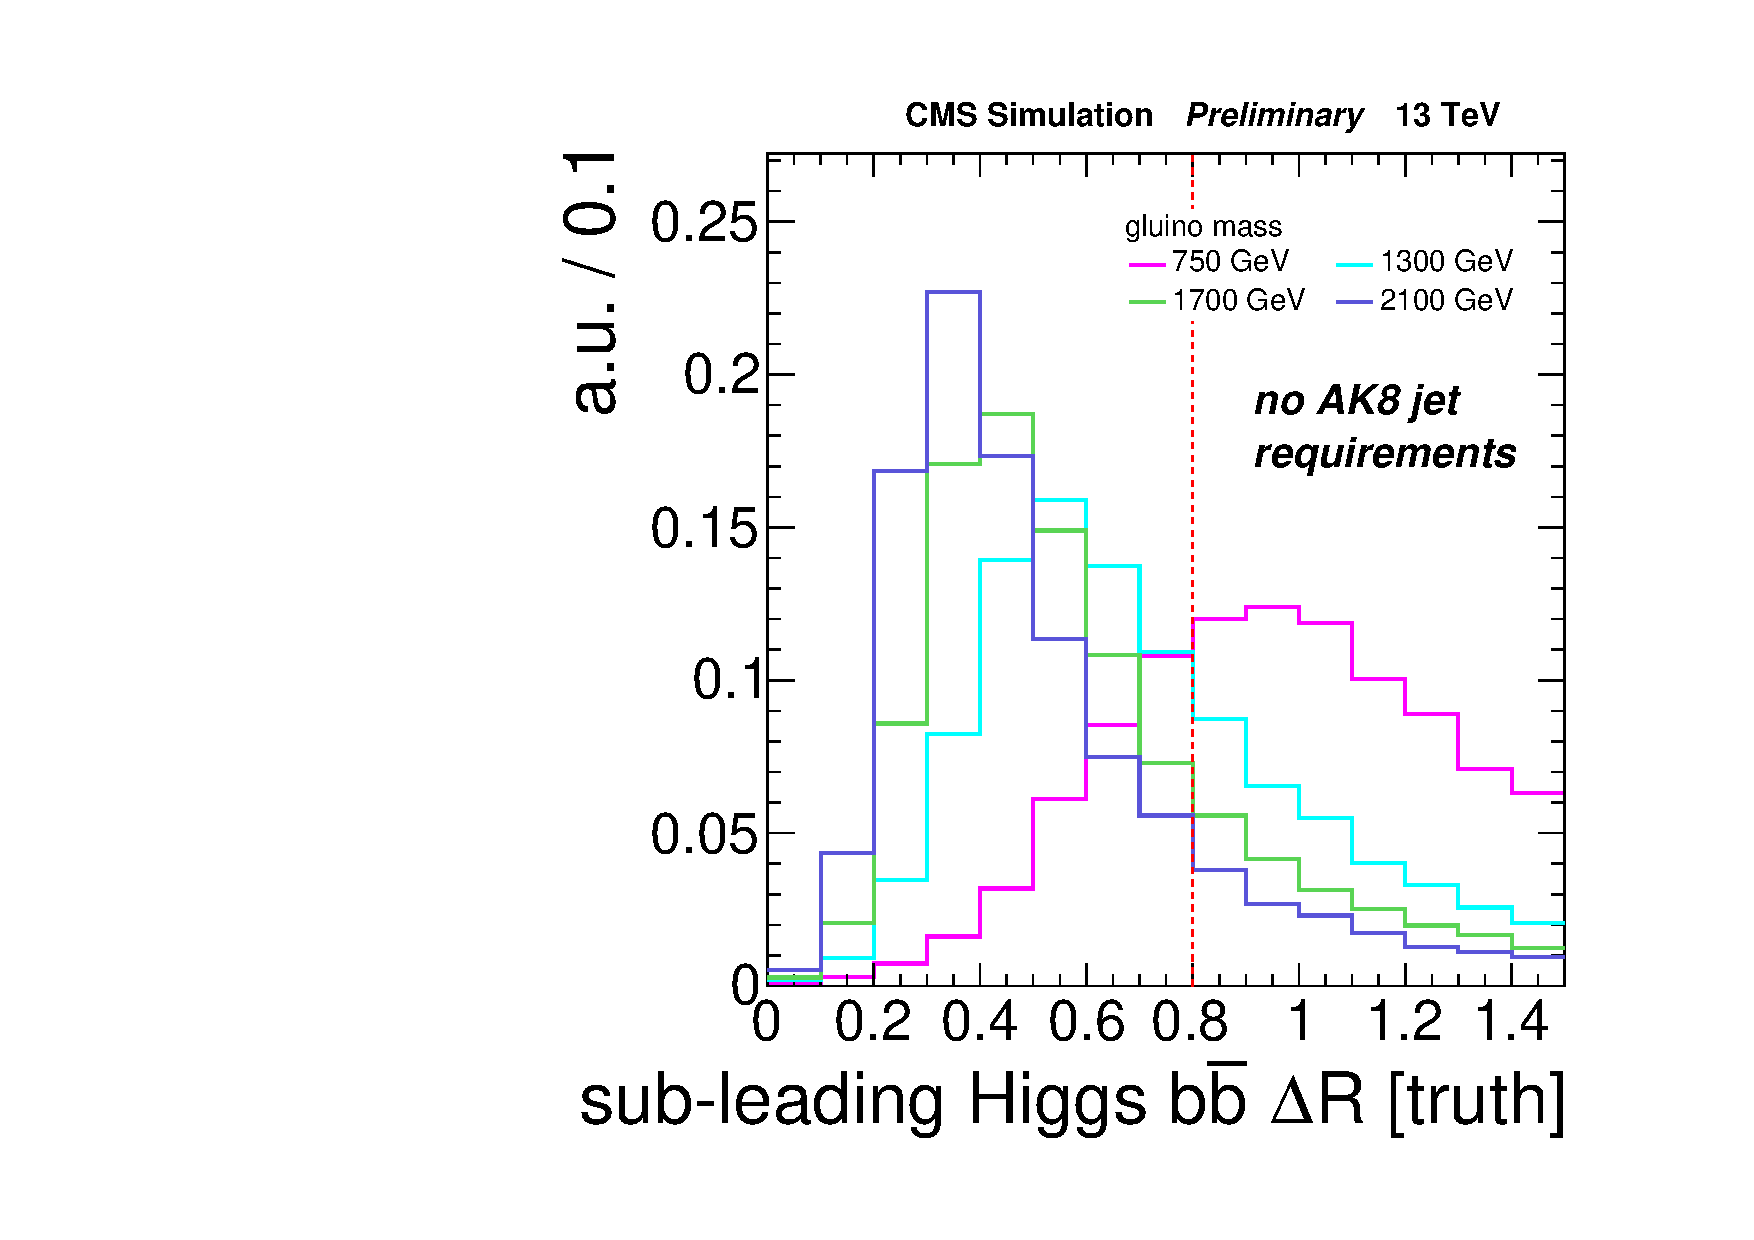
\includegraphics[width=0.45\linewidth]{figs/SUS17006/subleadHiggsDr.pdf}\\
\caption{
Generator level distributions for the leading (top row) and subleading (bottom row) H boson in the T5HH model. The plot on the left shows the $p_{T}$ of the H boson. The plot on right shows $\Delta R$ between the b-quark daughters - for large H $p_{T}$ the daughters become collimated.
}
\label{fig:GenHiggsBoost}
\end{figure}

\section{Event Binning \& Background Estimation}

The background estimation procedure makes use of what is known as an ``ABCD'' prediction in which the analysis phase space is divided into signal and sideband regions; scaling relations are applied to sideband yields to make predictions for the SM background (inclusive in all processes) in the signal regions. The events are categorized according to whether the AK8 jets are a) in the signal or sideband mass region and b) have or have not been $\mathrm{b}\bar{\mathrm{b}}$ tagged.  A diagram of this partitioning is seen in Figure \ref{fig:abcd}. An additional dimension is added by binning in \ptmiss: [300, 500 GeV], [500, 700 GeV], [700, $\infty$ GeV]. This gives a total of 2x3=6 signal and 4x3=12 sideband bins. The two signal regions $\mathrm{A}_{1, 2}$ contain events with one (and only one) or two jets being consistent with H/Z boson decay, respectively.

\begin{figure}
\centering
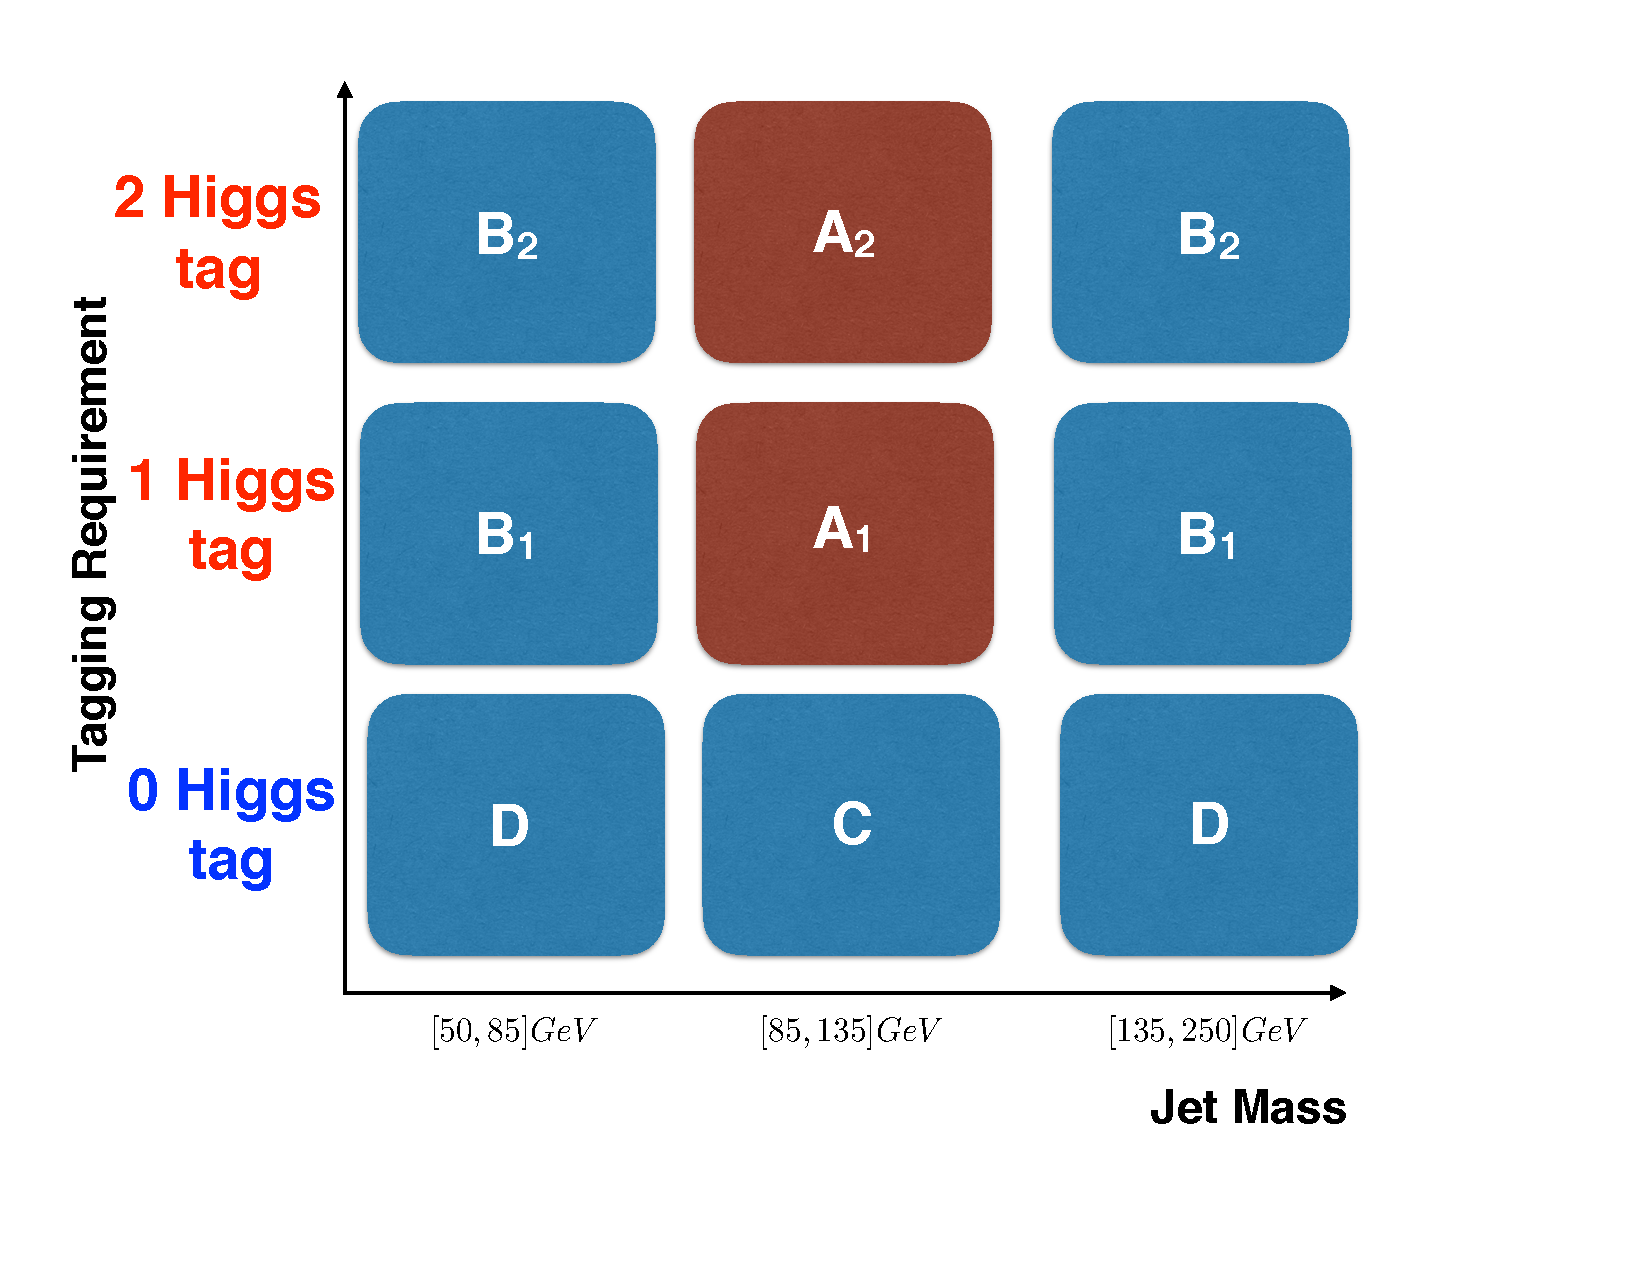
\includegraphics[width=0.6\textwidth]{figs/SUS17006/CMS-SUS-17-006_Figure-aux_002.pdf}
\caption{A diagram of the partitioned phase space. An additional binning in \ptmiss brings the number of analysis bins to 6x3=18.}
\label{fig:abcd}
\end{figure}

Assuming that there is no correlation between the jet mass and the $b\bar{b}$ tagging one would expect that

\begin{equation}
\frac{\mathrm{A}_{1, 2}}{\mathrm{B}_{1, 2}} = \frac{\mathrm{C}}{\mathrm{D}}
\end{equation}

Rearranging this gives a prediction for the events in the signal regions

\begin{equation}
\mathrm{A}_{1, 2}^{\mathrm{predicted}} = (\mathrm{B}_{1, 2} \cdot \frac{\mathrm{C}}{\mathrm{D}})^{\mathrm{observed}}
\end{equation}

The expected \ptmiss distribution from simulation is seen in the stacked histograms of Figure \ref{fig:mcclosure}. The prediction using the ABCD method is seen in the red hash. The expected level of closure in simulation can be determined by dividing the prediction in the signal region with the true content. This ratio, denoted $\kappa$, is seen in the bottom panel of Figure \ref{fig:mcclosure}. As will be discussed in Section \ref{sec:kappa}, $\kappa$ is used as a correction in the background estimation procedure.

\begin{figure}
\begin{subfigure}[b]{0.5\textwidth}
\centering
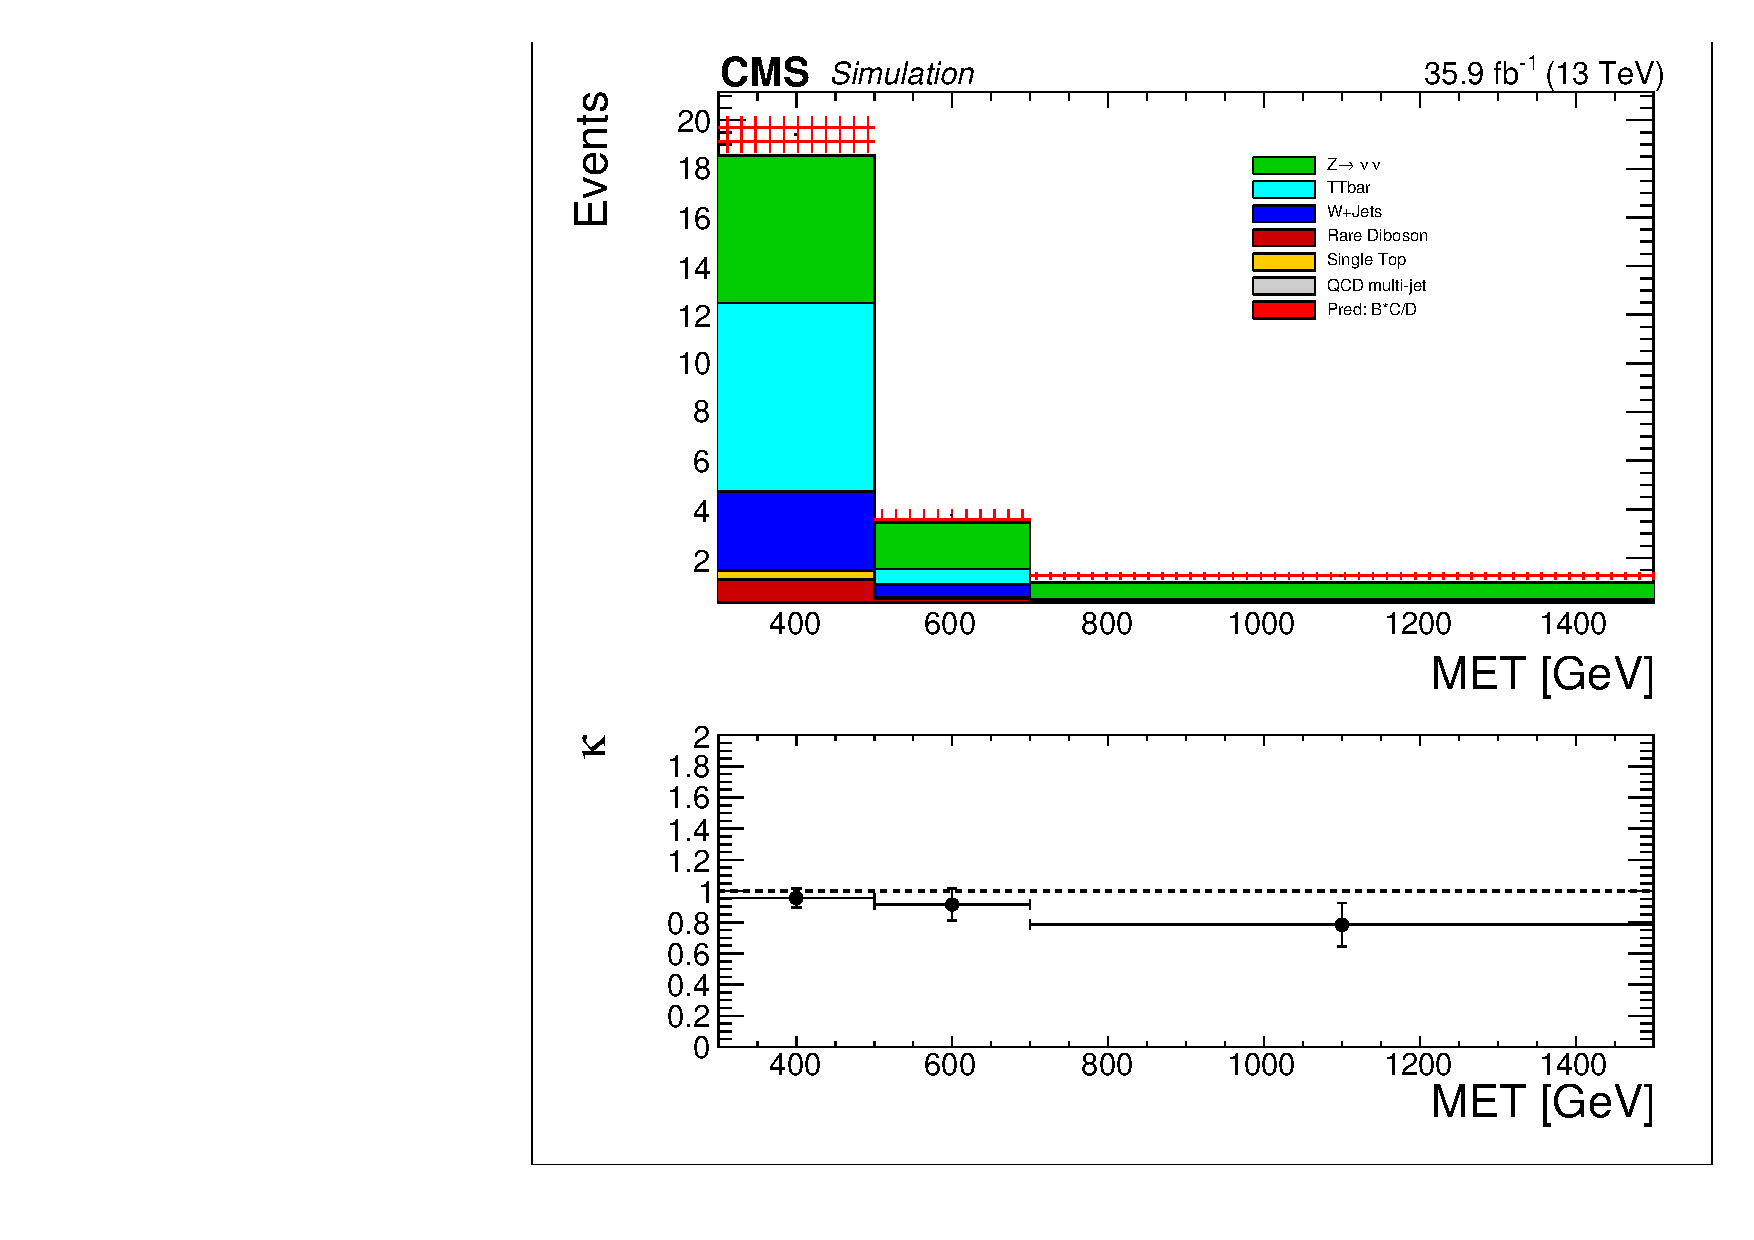
\includegraphics[trim={5px 5px 5px 5px},clip,width=\textwidth]{figs/SUS17006/MCclosure_singleHiggsRegionTotal.pdf}
\caption{The single Higgs tag region (A$_{1}$).}
\end{subfigure}
\begin{subfigure}[b]{0.5\textwidth}
\centering
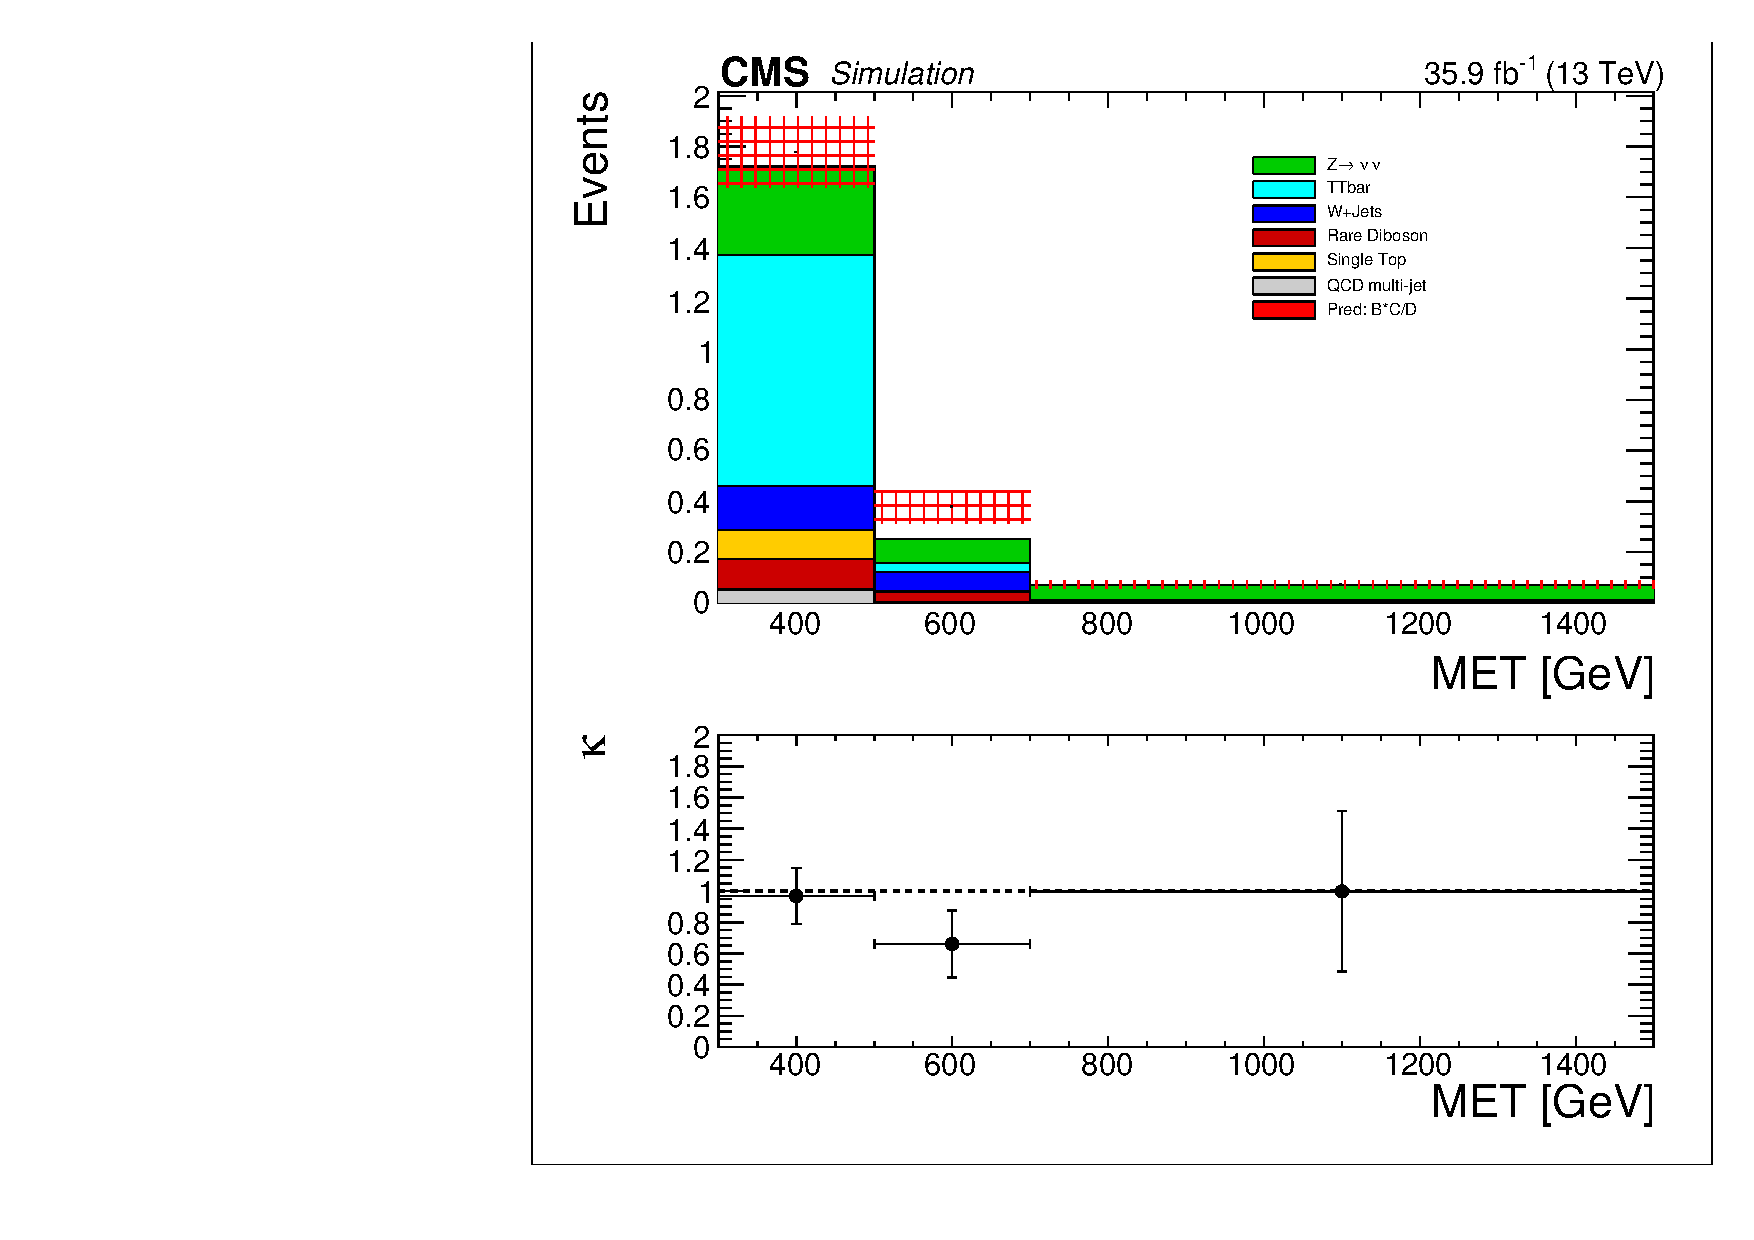
\includegraphics[trim={5px 5px 5px 5px},clip,width=\textwidth]{figs/SUS17006/MCclosure_doubleHiggsRegionTotal.pdf} 
\caption{The double Higgs tag region (A$_{2}$).}
\end{subfigure}
\caption{\ptmiss distributions and predictions in the signal regions using simulation only.}
\label{fig:mcclosure}
\end{figure}

\subsection{Study of the SM Background}
\label{sec:smbkg}

We treat the SM backgrounds in the signal region as consisting of three main components:
\begin{itemize}
\item $Z\rightarrow\nu\bar{\nu}$ in which the invisible Z gives true \ptmiss (`Z-invisible').
\item Semi-leptonic W or t production in which the lepton is not identified, the associated neutrino from the leptonic decay creates true \ptmiss (`lost-lepton').
\item Jet production via QCD in which the $p_{T}$ of a jet is substantially under-measured, this creates a fake source of \ptmiss.
\end{itemize}

To understand these backgrounds in data, three control regions were defined to serve as a proxy for each source.
\begin{itemize}
\item A single-photon control region, after artificially removing the photon from event reconstruction, closely mimics the Z-invisible background. For high-$p_{T}$, both photons and Z bosons become massless, neutral, gauge bosons whose kinematics are expected to be similar.
\item The single-lepton control region mimics the lost-lepton background.
\item The low-$\Delta\phi$ control region most closely mimics the QCD background. This selects events in which \ptmiss is aligned with an AK4 jet, enriching the sample with events in which a jet was mis-measured.
\end{itemize}

\subsection{Closure of the Estimation Within the Data Control Regions}

As they are orthogonal to our signal regions, we are able to test the closure of the background estimation technique independently in each of the three control regions. By comparing the prediction of the SM yields (using the ABCD method) with those observed in the signal-like bins, the validity of the technique can be verified for that particular background category. The comparisons for the single-photon, single-lepton and low-$\Delta\phi$ control regions can be seen in Figures \ref{fig:closurephoton}, \ref{fig:closuresinglelep}, \ref{fig:closurelowdphi}, respectively. $\kappa$ in bottom panel is defined as the ratio of the prediction to the true event yield (as usual). These comparisons are used for validation of the background estimation technique only, they are not used in the estimation.

\begin{figure}
\begin{subfigure}[b]{0.5\textwidth}
\centering
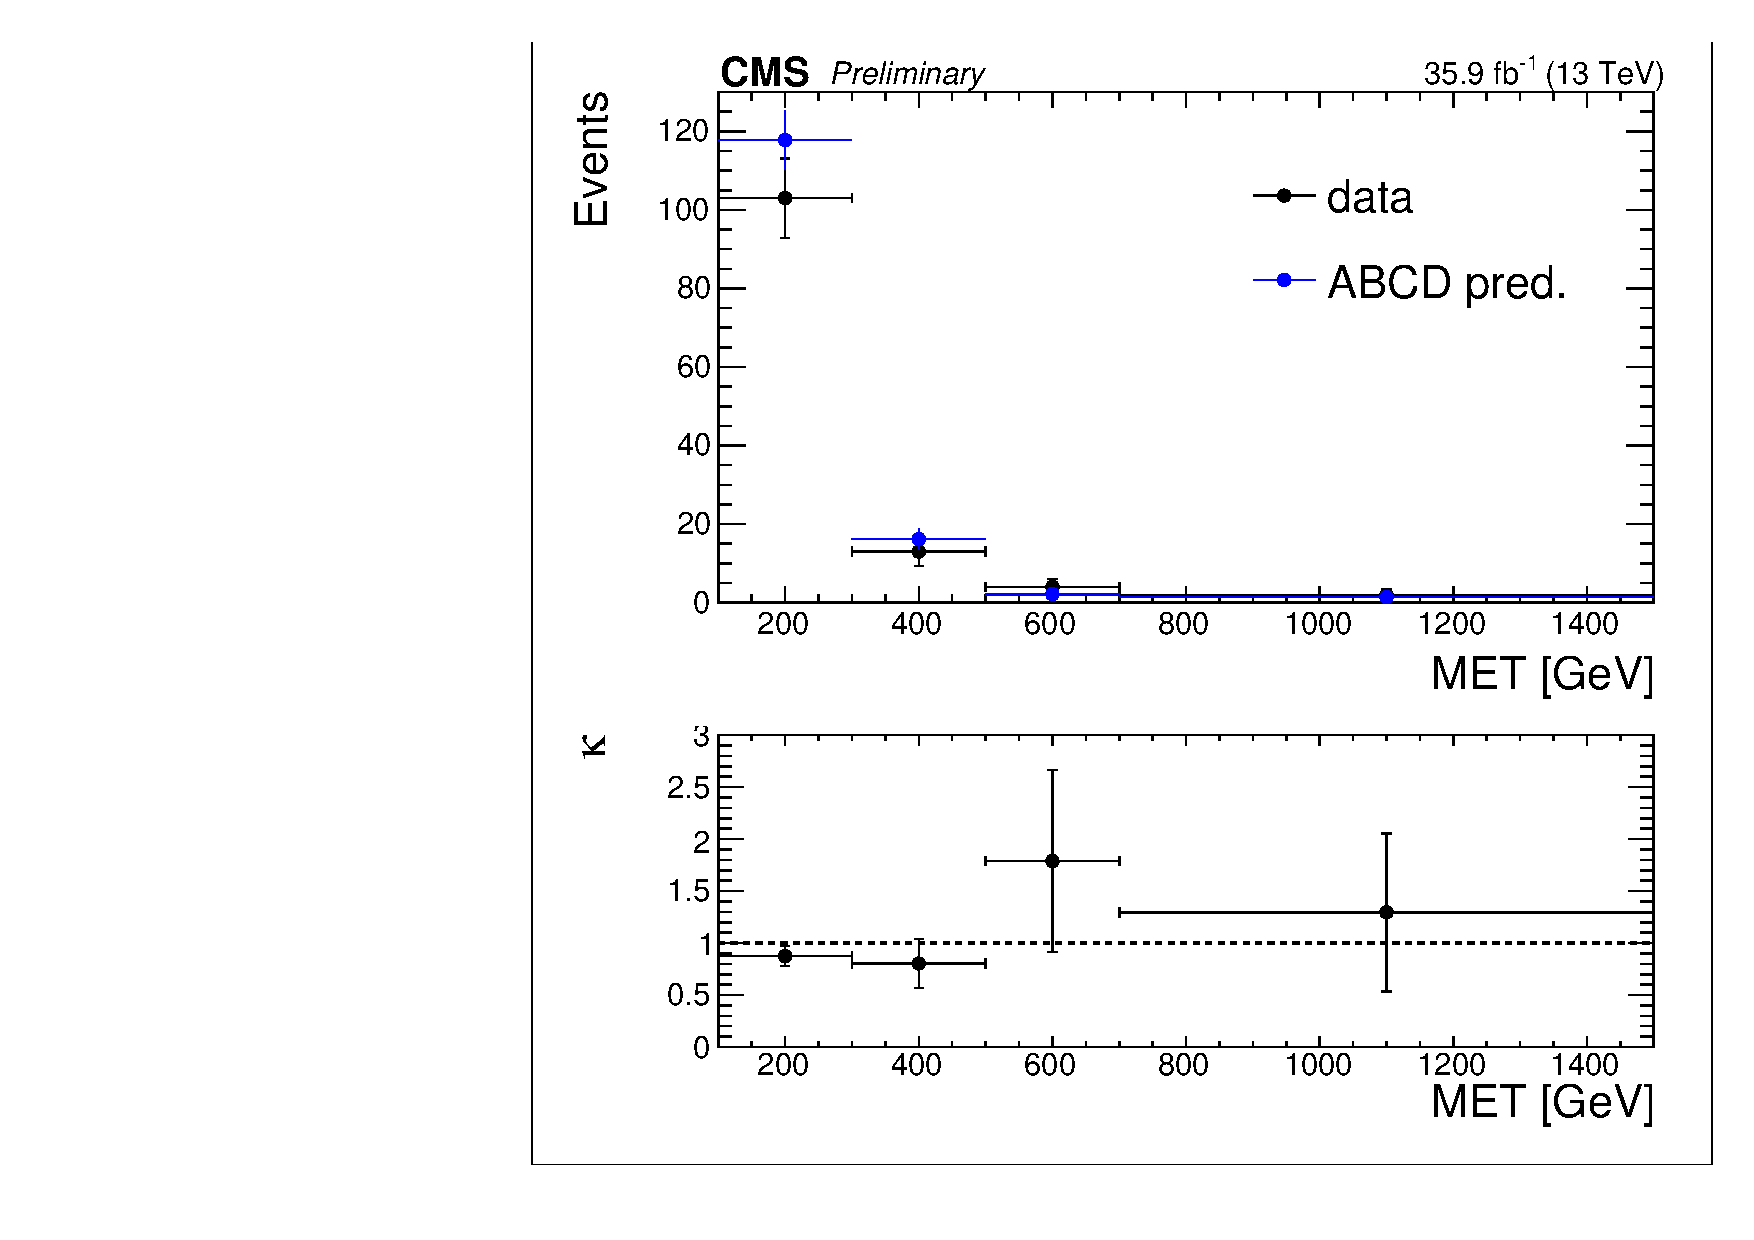
\includegraphics[trim={5px 5px 5px 5px},clip,width=\textwidth]{figs/SUS17006/dataClosure_single-tagSR_photon.pdf}
\caption{The single Higgs tag region (A$_{1}$).}
\end{subfigure}
\begin{subfigure}[b]{0.5\textwidth}
\centering
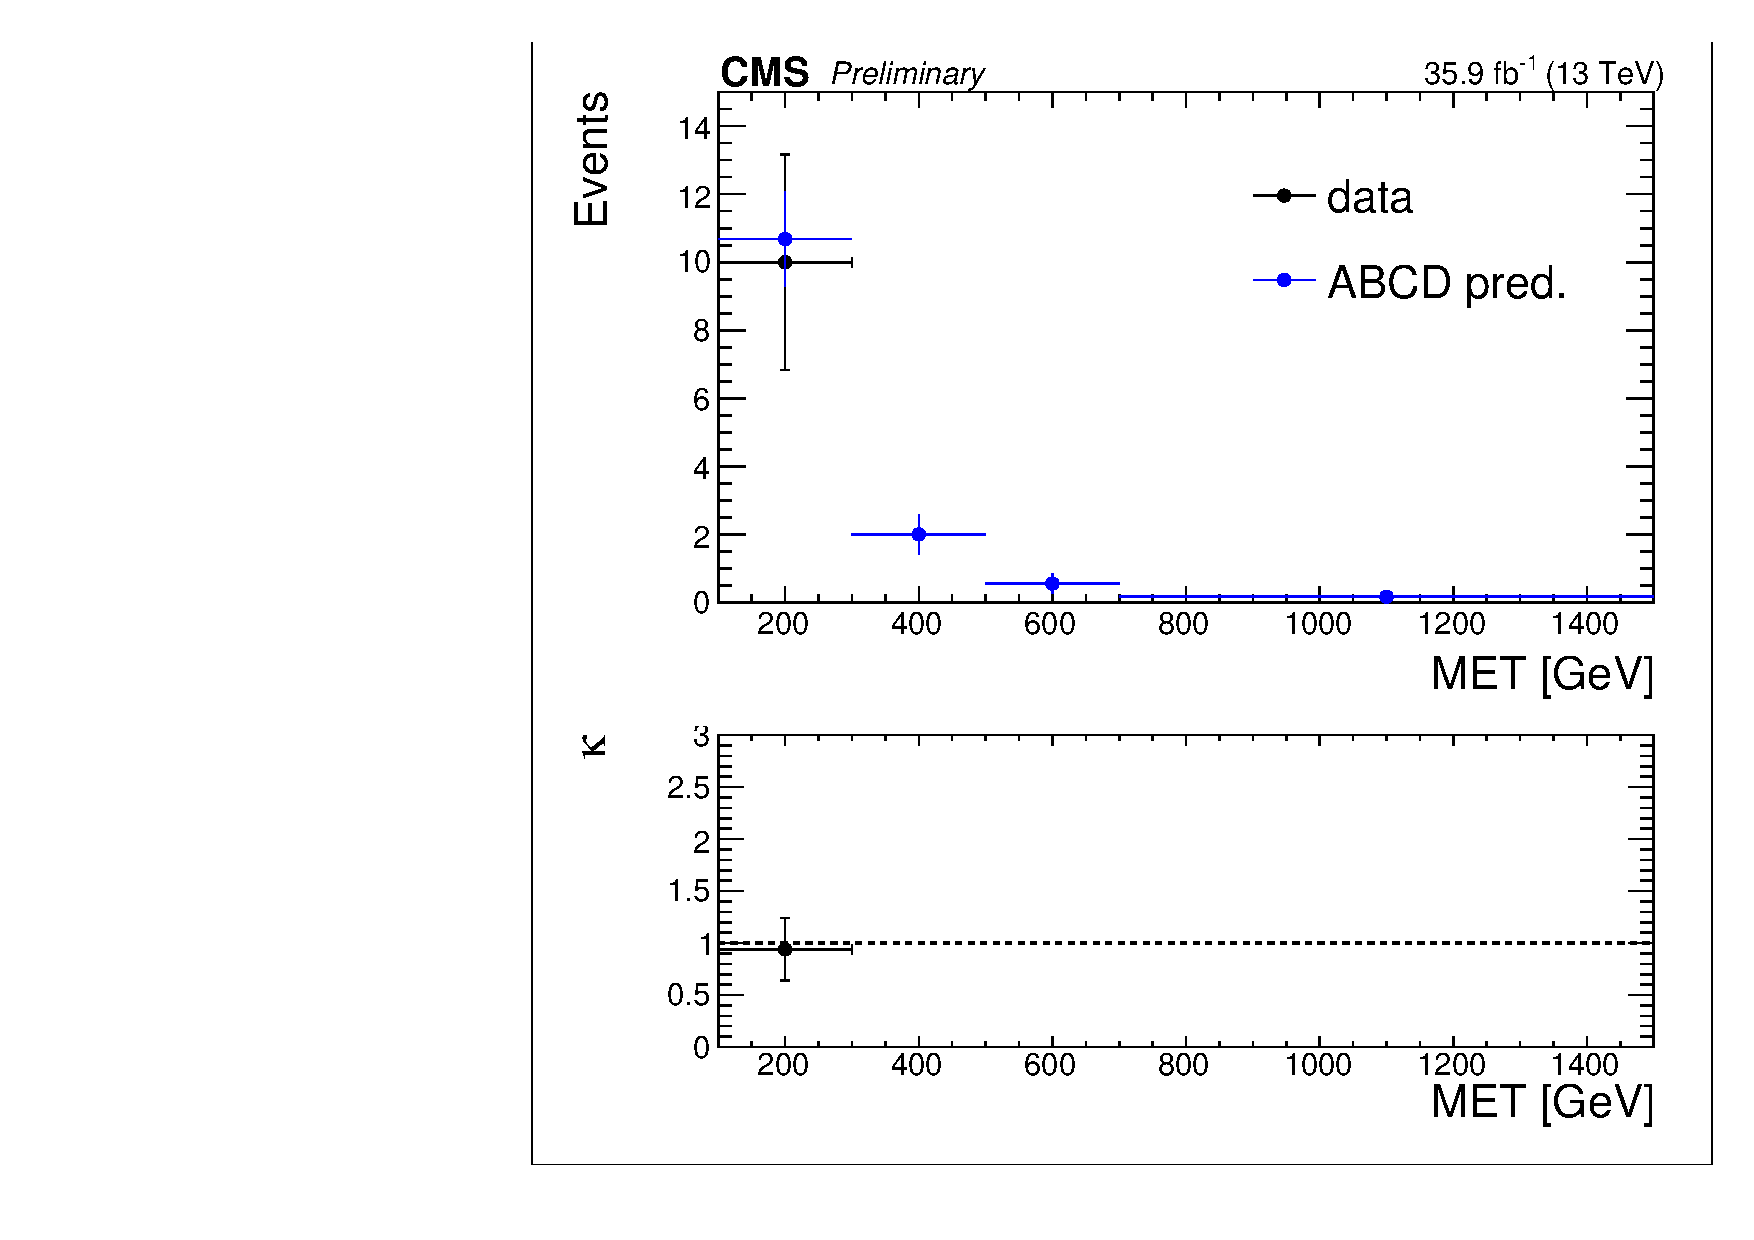
\includegraphics[trim={5px 5px 5px 5px},clip,width=\textwidth]{figs/SUS17006/dataClosure_double-tagSR_photon.pdf} 
\caption{The double Higgs tag region (A$_{2}$).}
\end{subfigure}
\caption{Closure within the single-photon data control region.}
\label{fig:closurephoton}
\end{figure}

\begin{figure}
\begin{subfigure}[b]{0.5\textwidth}
\centering
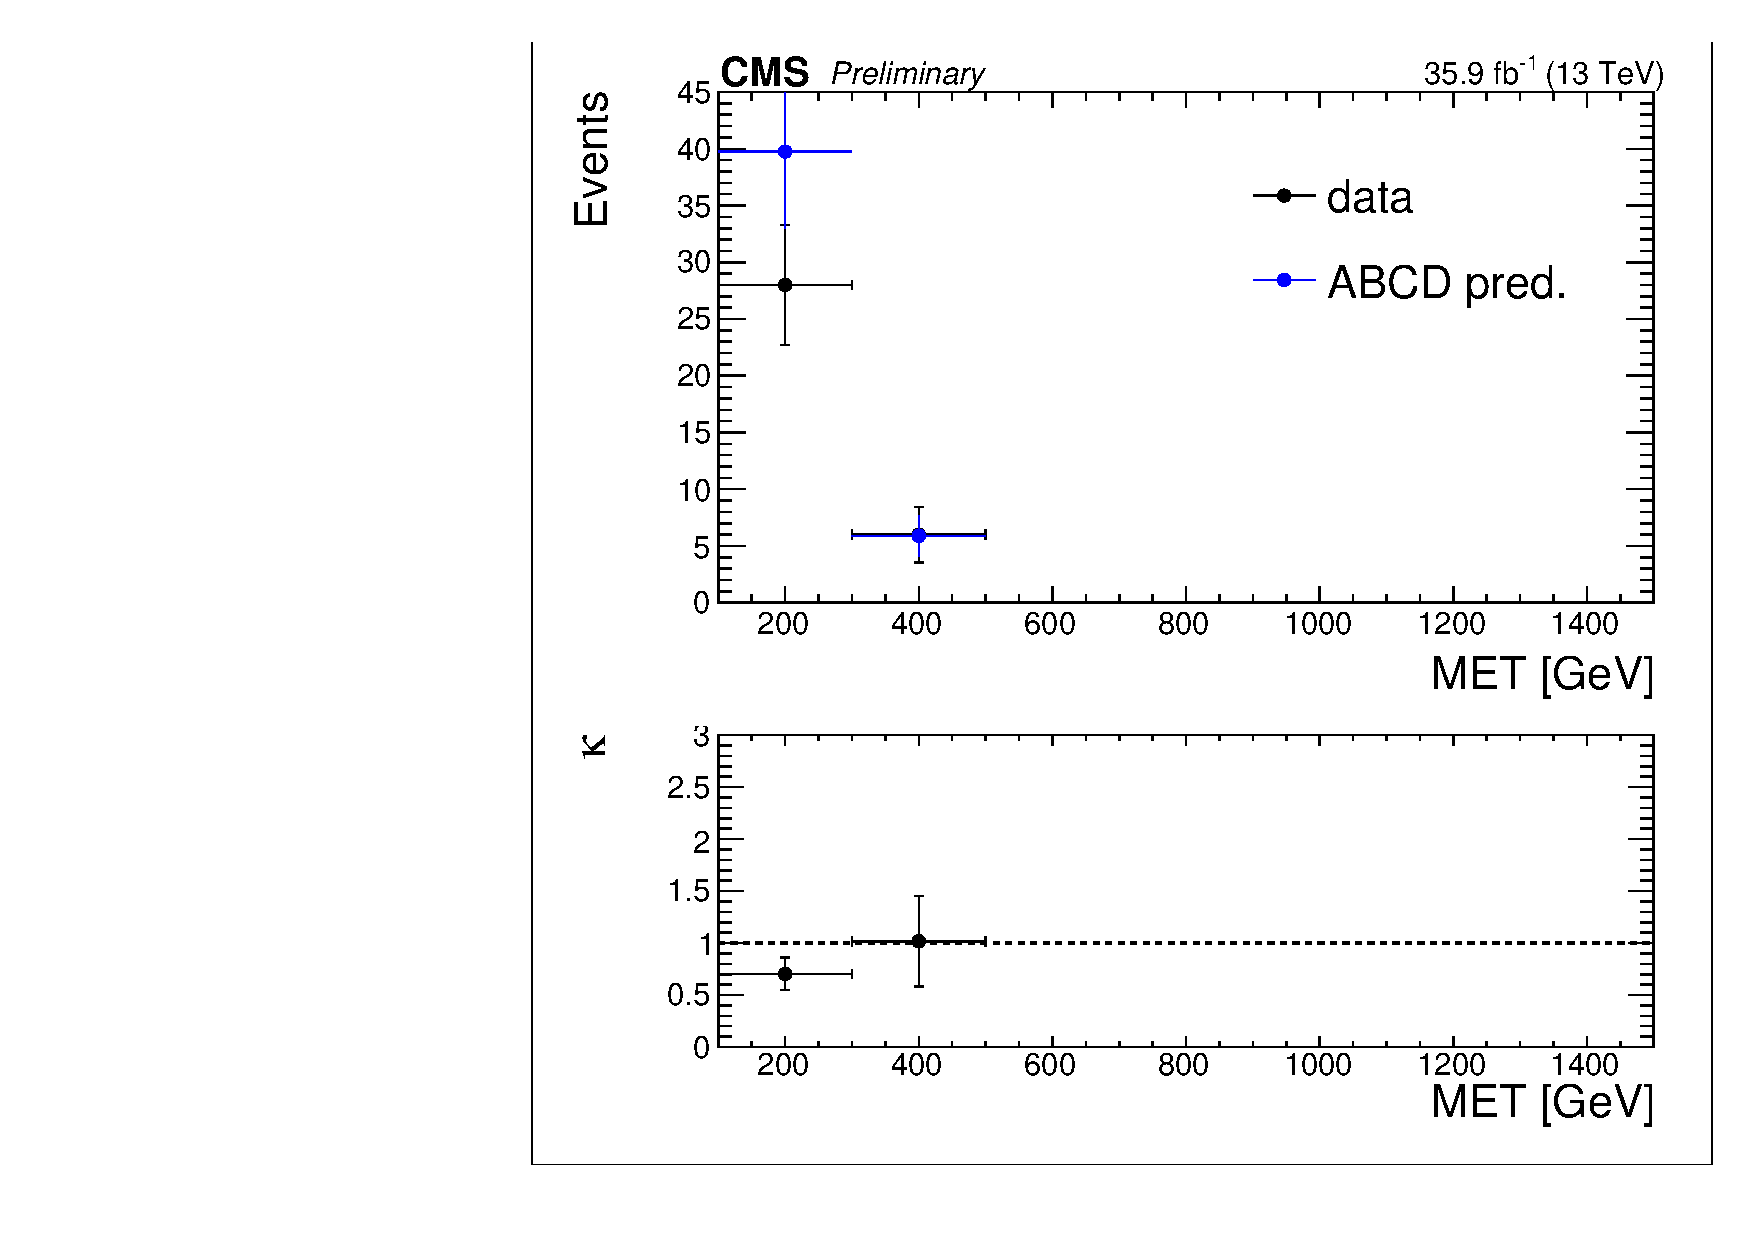
\includegraphics[trim={5px 5px 5px 5px},clip,width=\textwidth]{figs/SUS17006/dataClosure_single-tagSR_singleLep.pdf}
\caption{The single Higgs tag region (A$_{1}$).}
\end{subfigure}
\begin{subfigure}[b]{0.5\textwidth}
\centering
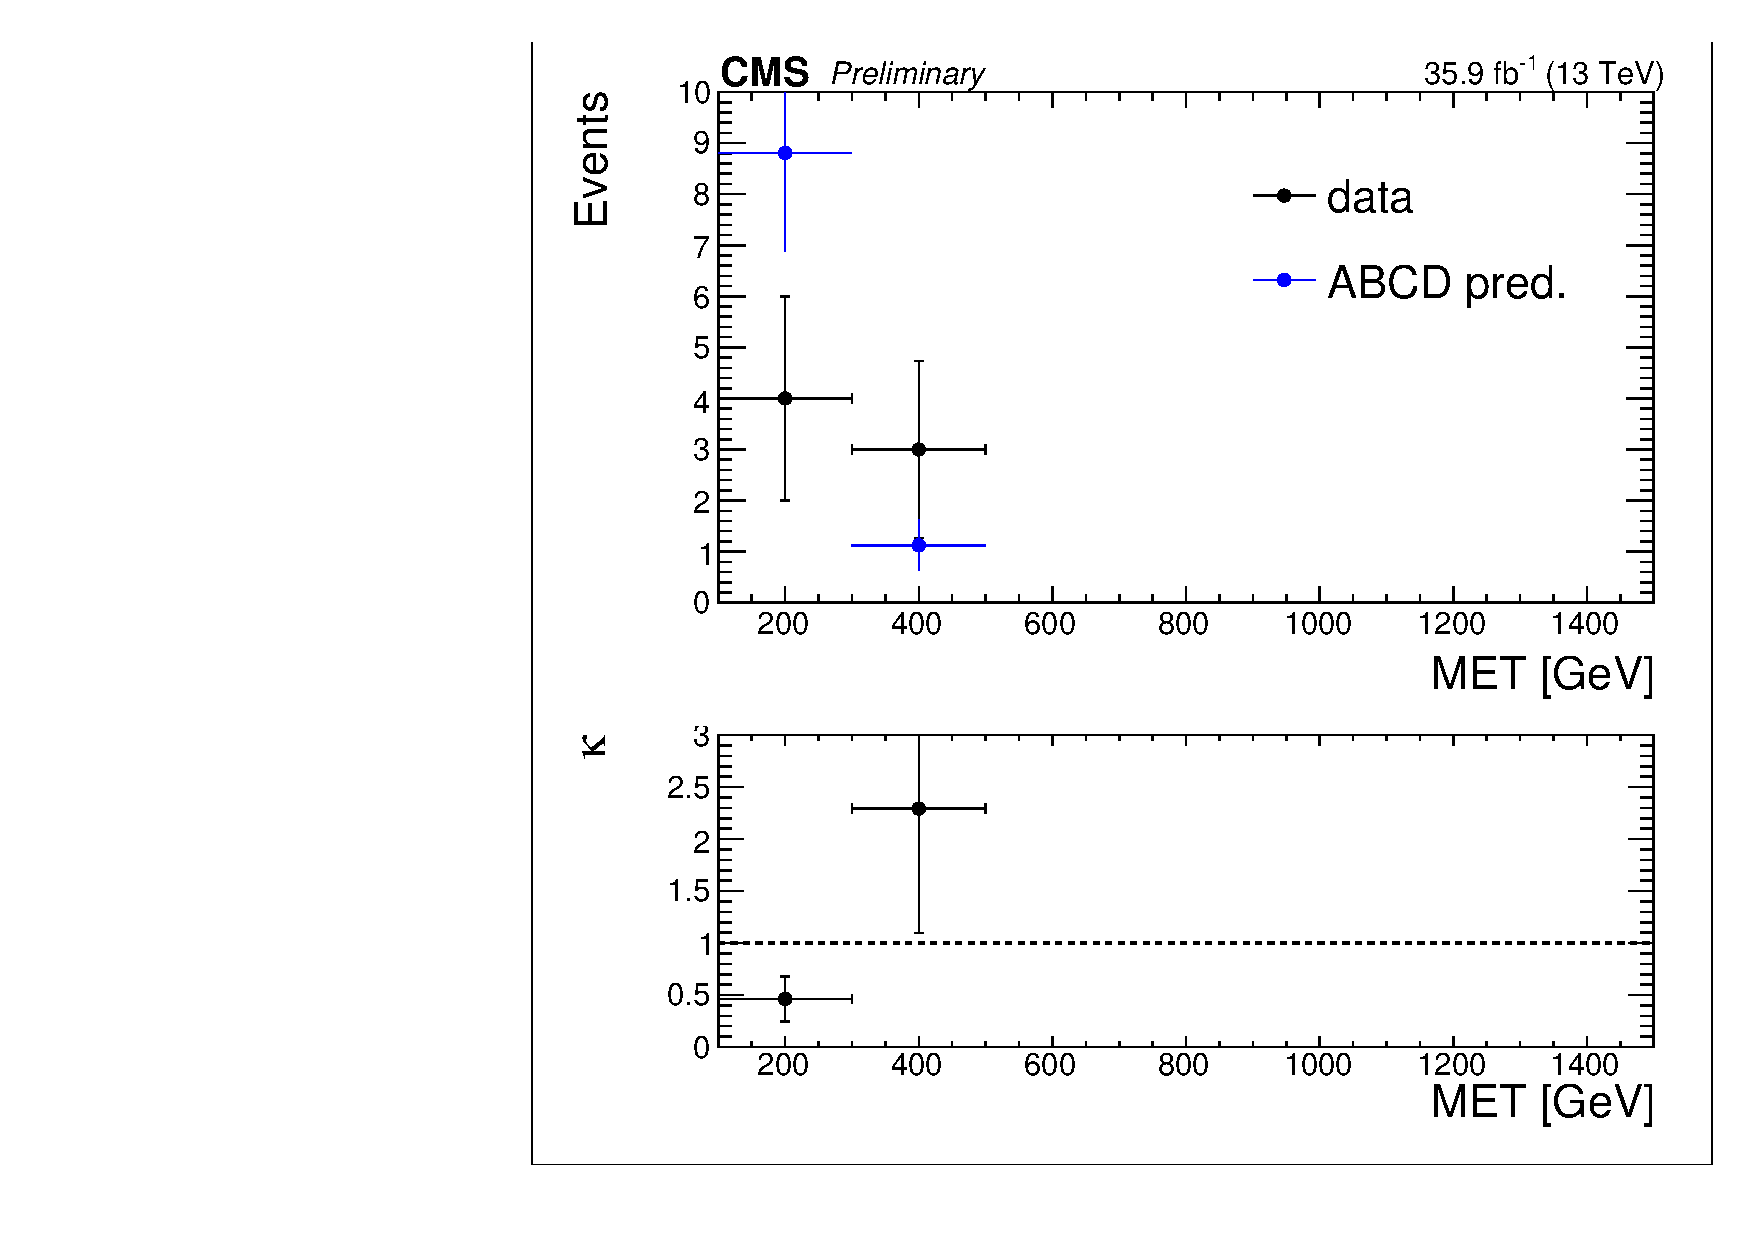
\includegraphics[trim={5px 5px 5px 5px},clip,width=\textwidth]{figs/SUS17006/dataClosure_double-tagSR_singleLep.pdf} 
\caption{The double Higgs tag region (A$_{2}$).}
\end{subfigure}
\caption{Closure within the single-lepton (e, $\mu$) data control region.}
\label{fig:closuresinglelep}
\end{figure}

\begin{figure}
\begin{subfigure}[b]{0.5\textwidth}
\centering
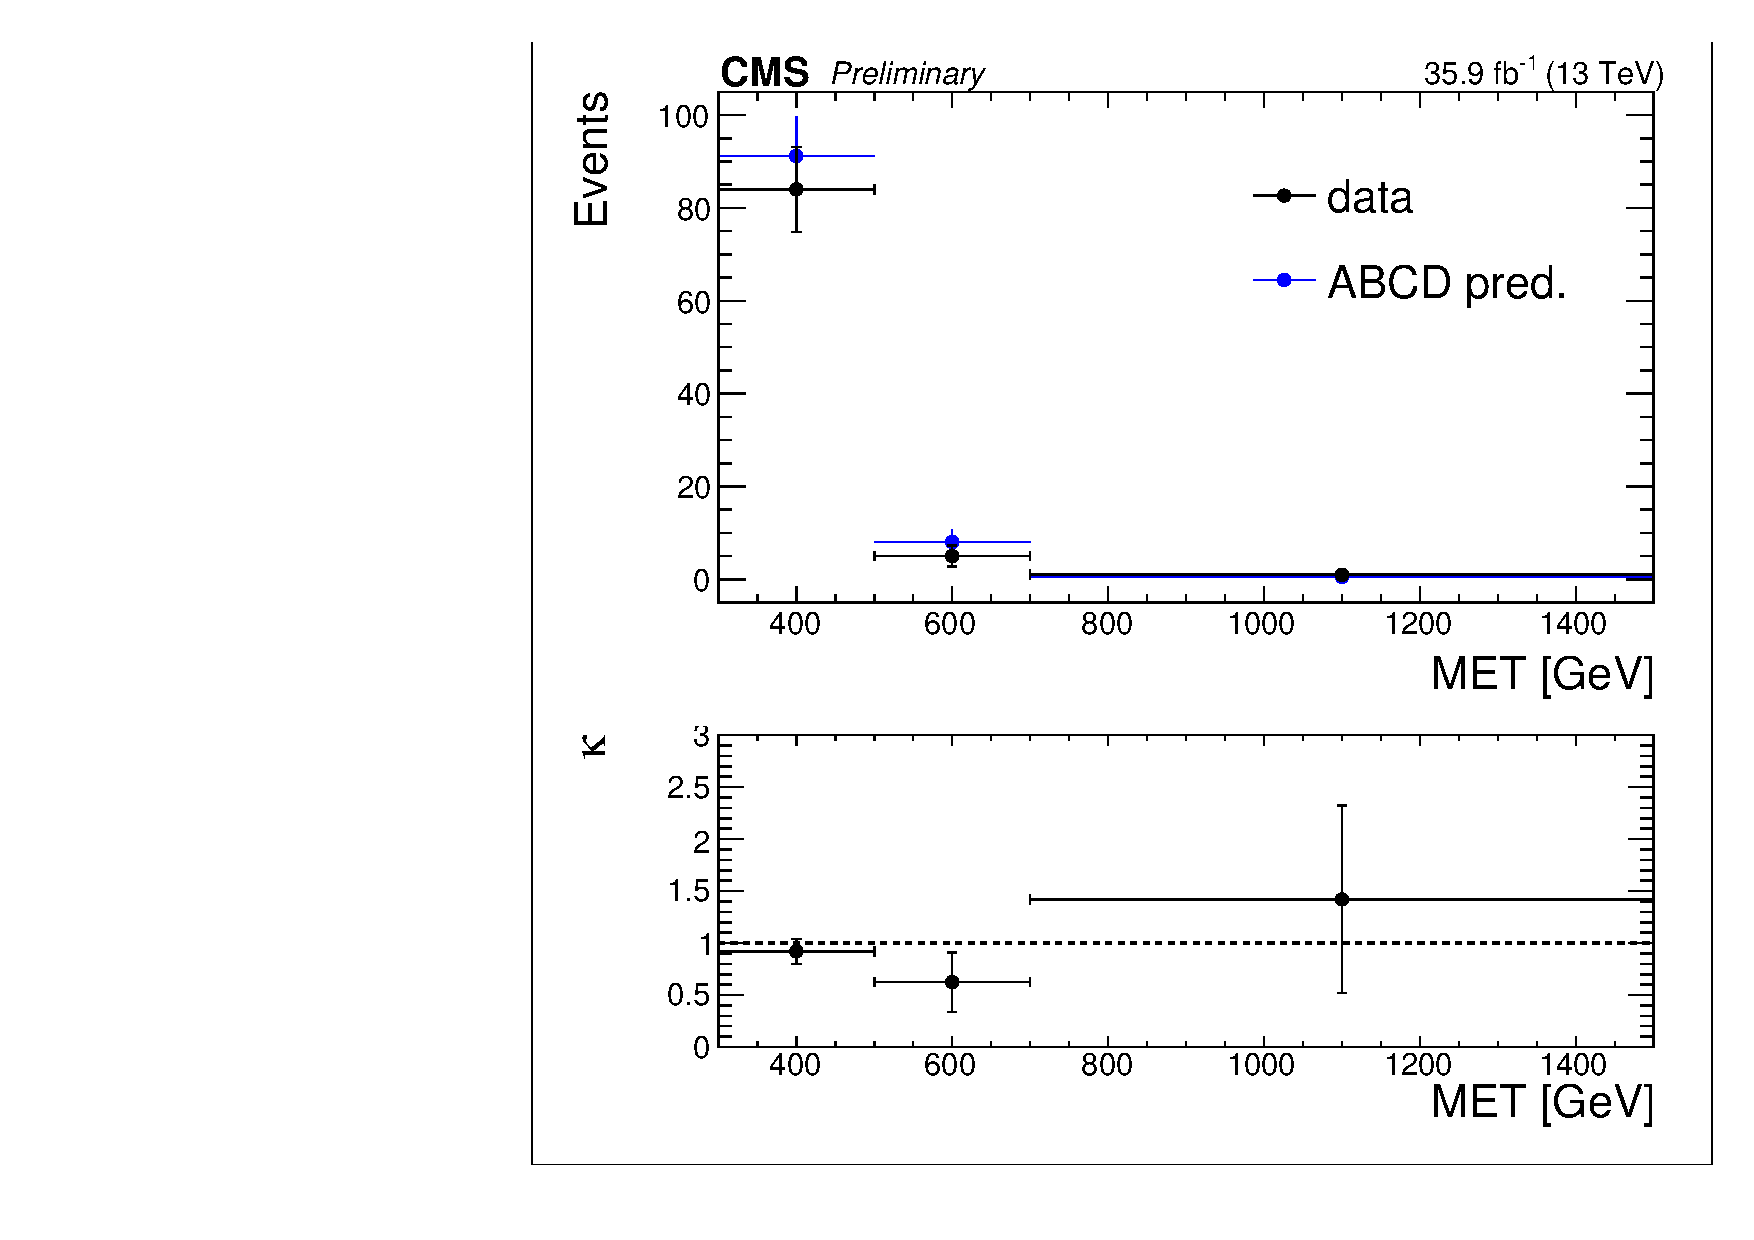
\includegraphics[trim={5px 5px 5px 5px},clip,width=\textwidth]{figs/SUS17006/dataClosure_single-tagSR_lowDphi.pdf}
\caption{The single Higgs tag region (A$_{1}$).}
\end{subfigure}
\begin{subfigure}[b]{0.5\textwidth}
\centering
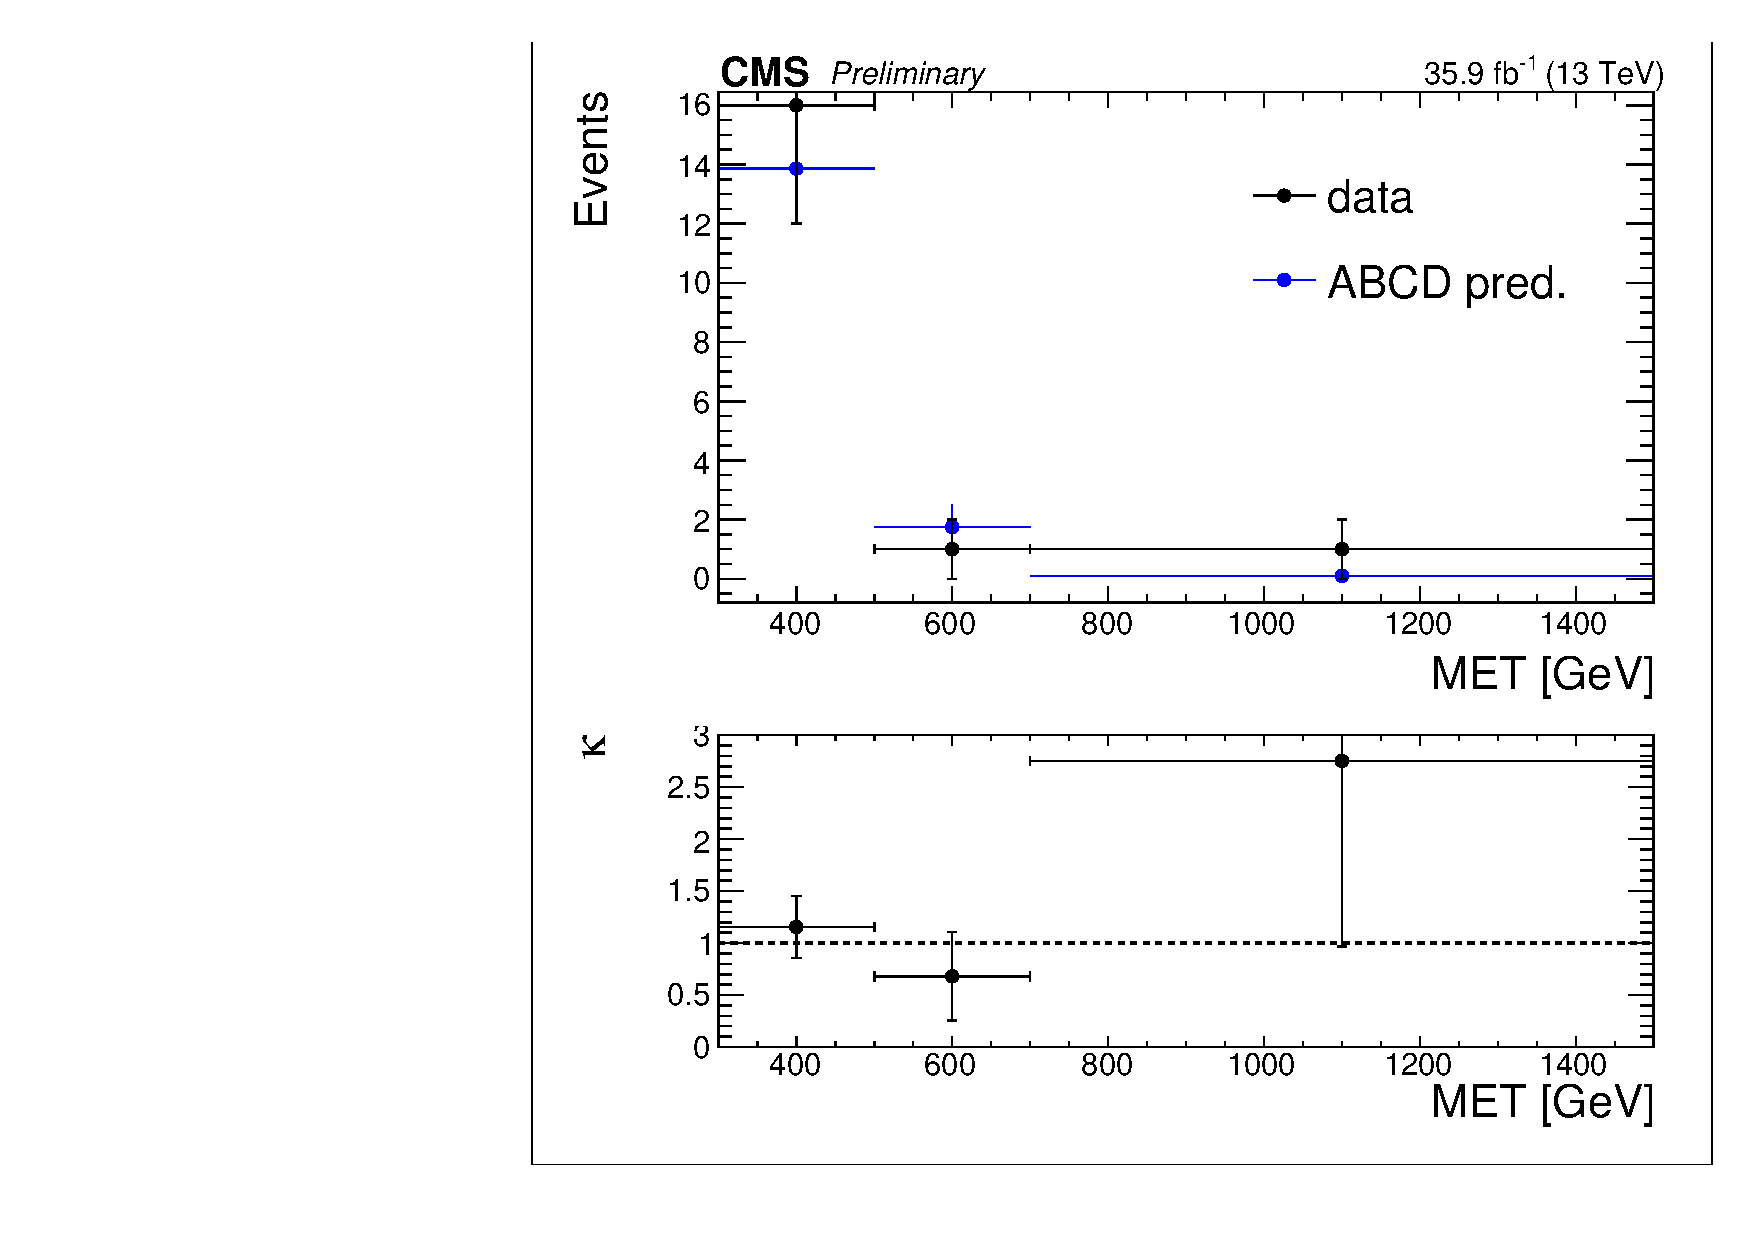
\includegraphics[trim={5px 5px 5px 5px},clip,width=\textwidth]{figs/SUS17006/dataClosure_double-tagSR_lowDphi.pdf} 
\caption{The double Higgs tag region (A$_{2}$).}
\end{subfigure}
\caption{Closure within the low-$\Delta\phi$ data control region.}
\label{fig:closurelowdphi}
\end{figure}

\subsection{$\kappa$ as a Correction to the Estimation}
\label{sec:kappa}

To correct for the observed non-closure of the background estimation method a correction $\kappa$ is applied to the SM background prediction. $\kappa$ is obtained by dividing the MC yields for the signal region by that predicted:

\begin{equation}
\kappa  \equiv A_{1, 2}^{mc} \,/  \ (B_{1, 2} \cdot \ \frac{C} {D} \ )^{mc}
\end{equation}

There are 2x3=6 values of $\kappa$, one for each signal bin. The corrections are then applied as follows:

\begin{equation}
A_{1, 2}^{\mathrm{predicted}} = \kappa \cdot (B_{1, 2} \cdot \ \frac{C}{D})^{\textrm{observed}}
\end{equation}

These values of $\kappa$ are those seen in Figure \ref{fig:mcclosure}.

The value of $\kappa$ is dependent on the yields of each analysis bin and is therefore sensitive to the accuracy of the modeling of MC in each bin. To improve the accuracy in the determination of $\kappa$ scale factors are derived using data to correct the normalization of MC in each bin. The fractional composition of the background predicted by MC before any such corrections is seen in Figure \ref{fig:composition}.

\begin{figure}
\begin{subfigure}[b]{0.42\textwidth}
\centering
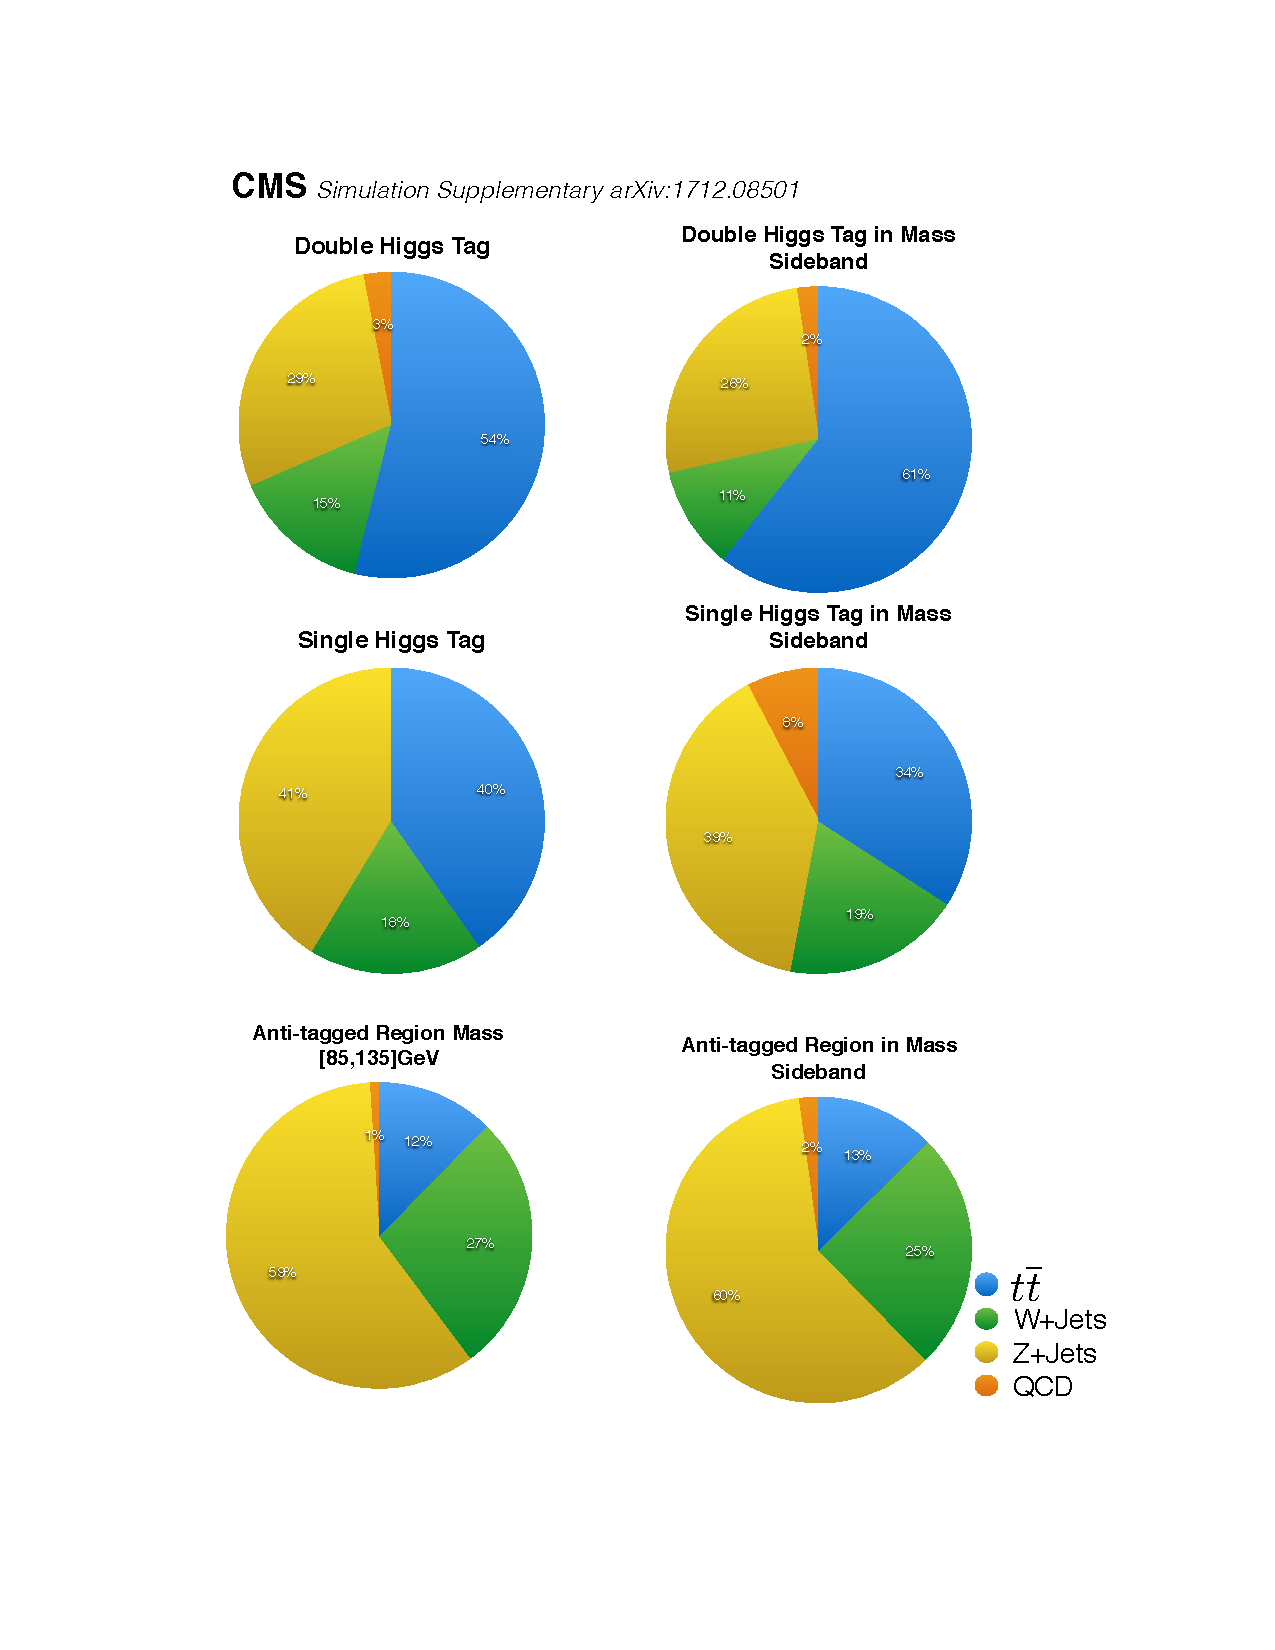
\includegraphics[width=\textwidth]{figs/SUS17006/CMS-SUS-17-006_Figure-aux_003.pdf}
\caption{The analysis bins inclusive in \ptmiss.}
\end{subfigure}
\begin{subfigure}[b]{0.58\textwidth}
\centering
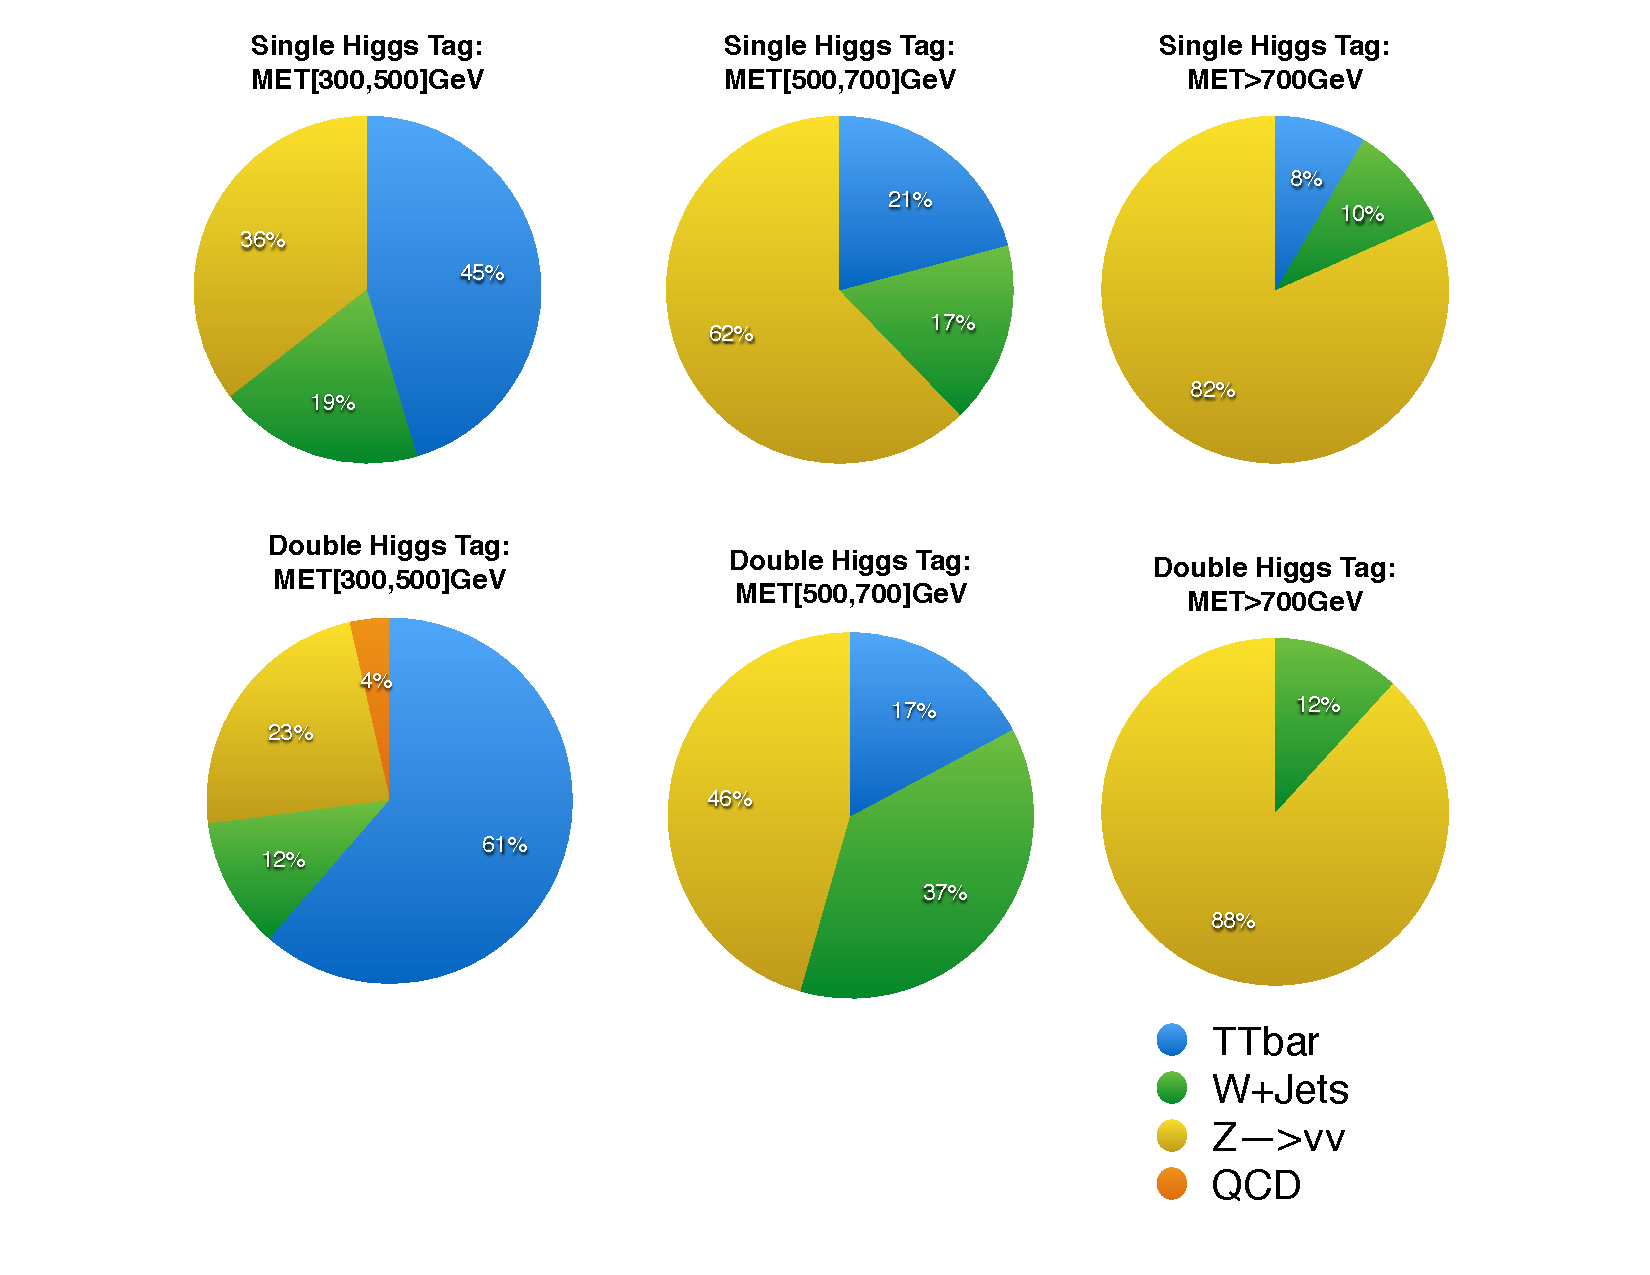
\includegraphics[width=\textwidth]{figs/SUS17006/PieChartBkgComp.pdf} 
\caption{$A_{1, 2}$ binned in \ptmiss.}
\end{subfigure}
\caption{Fractional composition of SM background in the analysis bins, as predicted by MC.}
\label{fig:composition}
\end{figure}

The scale factors are determined within the control regions by dividing the yields observed in data with those in MC. The dependence of the scale-factors on \ptmiss is studied in a looser phase-space with AK8 jet $p_{T}>170\,\textrm{GeV}$. The low-$\Delta\phi$ and single-photon scale factors show no \ptmiss dependence and are determined integrated over \ptmiss$>300\,\textrm{GeV}$. These are seen in Table \ref{tab:ScaleFactorVR}. The Single-lepton region does show \ptmiss dependence and are seen in Table \ref{tab:ScaleFactorMET}.

\begin{table}
\centering
\caption{Summary of the Validation region scale-factors derived integrated over the \ptmiss search bins. They are computed for each of the regions defined at the beginning of the Section.}
\begin{tabular}{c|c|c|c|c|c}
\hline \hline
\multicolumn{6}{c}{Low $\Delta\phi$}\\
\hline \hline
$A^{1H}_{SF}$ & $A^{2H}_{SF}$ & $C_{SF}$ & $B^{1}_{SF}$ & $B^{2}_{SF}$ & $D_{SF}$  \\ \hline
   $1.1 \pm 0.33$ &$0.85 \pm 0.12$&  $0.93 \pm 0.1$ & $0.88 \pm 0.04$ & $1.2 \pm 0.16$  & $0.71 \pm 0.027$ \\ \hline
\hline \hline
\multicolumn{6}{c}{Single Lepton}\\
\hline \hline
$A^{1H}_{SF}$ & $A^{2H}_{SF}$ & $C_{SF}$ & $B^{1}_{SF}$ & $B^{2}_{SF}$ & $D_{SF}$  \\ \hline
   %$0.63 \pm 0.069$ & $0.64 \pm 0.15$  & \MET dependent &   $0.65 \pm 0.1$ & $0.71 \pm 0.059$  & \MET dependent\\ \hline
   %$0.64 \pm 0.033$ & $0.68 \pm 0.068$  & \MET dependent &   $0.63 \pm 0.011$ & $0.72 \pm 0.023$  & \MET dependent\\ \hline
   $0.61\pm 0.04$ & $0.59\pm0.08$ & \ptmiss dependent &  $0.59\pm 0.016$ & $0.71\pm 0.04$  & \ptmiss dependent\\ \hline
\hline \hline
\multicolumn{6}{c}{Photon}\\
\hline \hline
$A^{1H}_{SF}$ & $A^{2H}_{SF}$ & $C_{SF}$ & $B^{1}_{SF}$ & $B^{2}_{SF}$ & $D_{SF}$ \\ \hline
   $0.61 \pm 0.088$ & $0.75 \pm 0.29$ & $0.5 \pm 0.07$ & $0.98 \pm 0.094$ & $2.58 \pm 0.63$ & $0.71 \pm 0.035$\\ \hline
\end{tabular}
\label{tab:ScaleFactorVR}
\end{table}

\begin{table}
\caption{Summary of the Single Lepton Validation region scale-factors for each of the \ptmiss bins in the anti-tag control regions.}
\centering
\begin{tabular}{|c|c|c|}
\hline\hline
\multicolumn{3}{c}{Single Lepton $C_{SF}$}\\
\hline
\ptmiss [300, 500] & [500, 700] & [700, $\infty$]\\
$0.47\pm0.05$ & $0.54\pm0.15$ & $0.18\pm 0.1$ \\  \hline\hline
\multicolumn{3}{c}{Single Lepton $D_{SF}$}\\
\hline
$0.49\pm0.02$ & $0.40\pm0.05$ & $0.35\pm 0.08$ \\  
\hline \hline
\end{tabular}
\label{tab:ScaleFactorMET}
\end{table}

These scale factors are then applied directly to the MC to check $\kappa$ with a composition that better reflects the data. The composition before such corrections are seen in Figure \ref{fig:composition}. Figure \ref{fig:mcclosuresf} shows the modified \ptmiss distributions in the 6 signal regions after correcting simulation with the scale factors derived from the data control regions. Since most of the scale factors are less than one the background decreases in Figure \ref{fig:mcclosure} relative to Figure \ref{fig:mcclosuresf} but still preserves closure so that $\kappa$ is statistically compatible with unity. A distribution of $\kappa$ is derived by throwing gaussian toys for each of the scale factors. We apply the scale factors from each toy to obtain a distribution of $\kappa$. 

\begin{figure}
\begin{subfigure}[b]{0.5\textwidth}
\centering
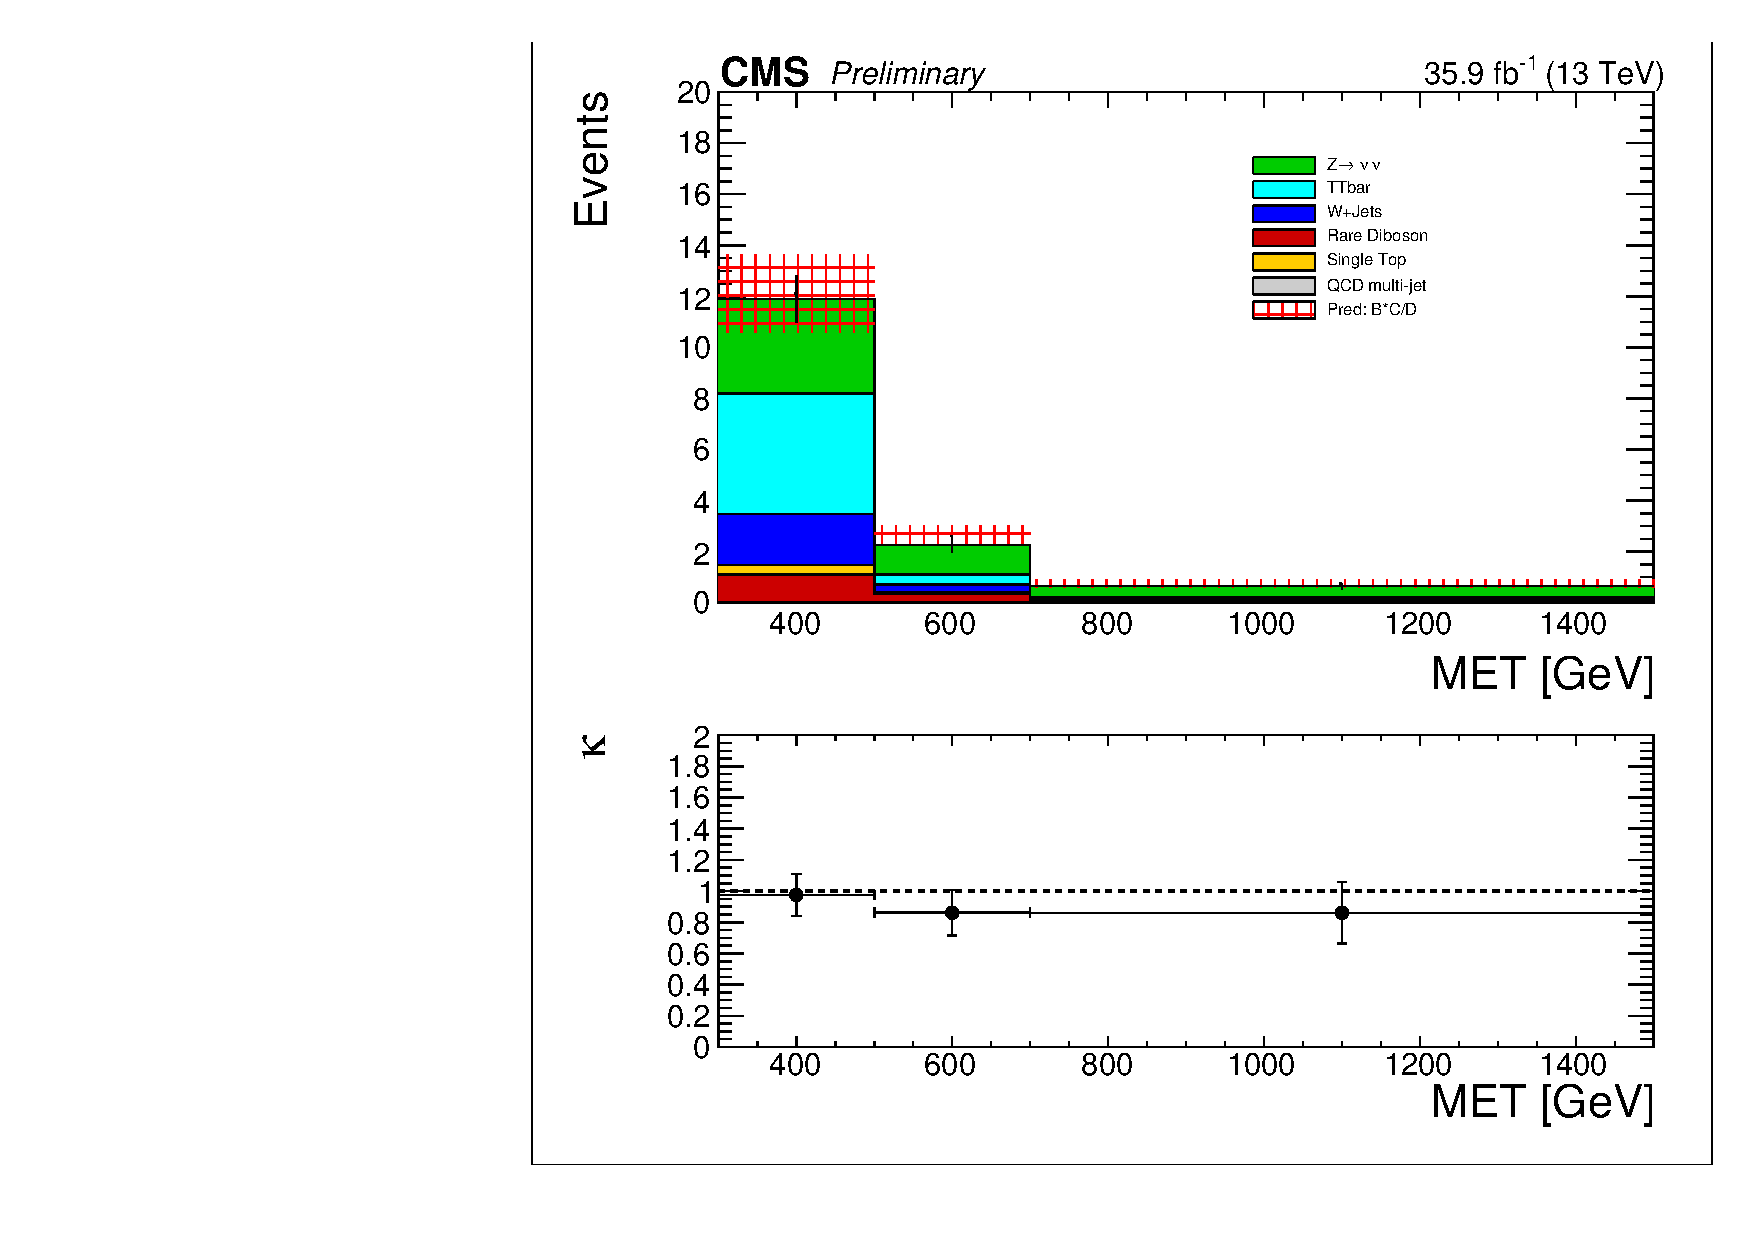
\includegraphics[trim={5px 5px 5px 5px},clip,width=\textwidth]{figs/SUS17006/MCclosureSF_singleHiggsRegionTotal.pdf}
\caption{The single Higgs tag region (A$_{1}$).}
\end{subfigure}
\begin{subfigure}[b]{0.5\textwidth}
\centering
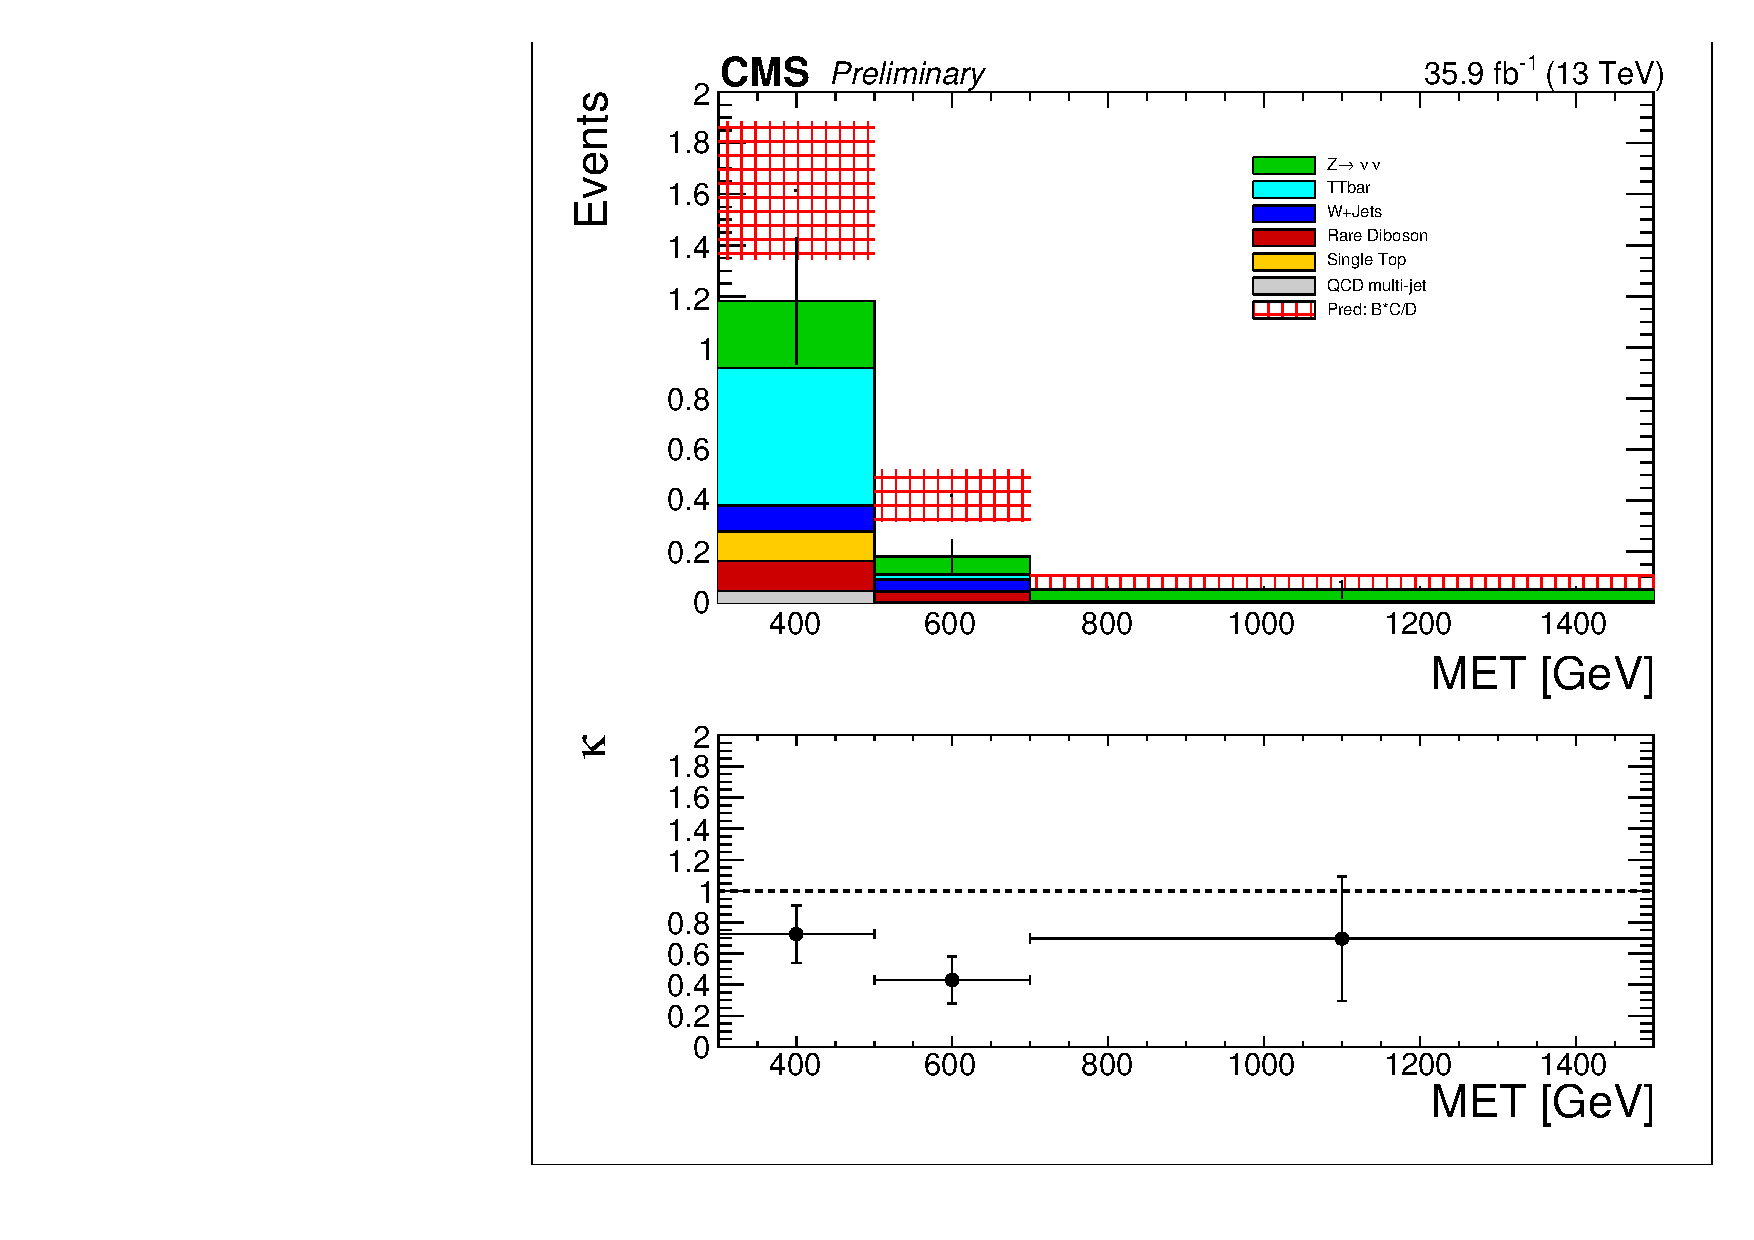
\includegraphics[trim={5px 5px 5px 5px},clip,width=\textwidth]{figs/SUS17006/MCclosureSF_doubleHiggsRegionTotal.pdf} 
\caption{The double Higgs tag region (A$_{2}$).}
\end{subfigure}
\caption{\ptmiss distributions and the predictions in the signal regions using simulation with scale factors from data.}
\label{fig:mcclosuresf}
\end{figure}

\subsection{Sideband Yields \& Predictions}

Observed yields in data for the 4x3=12 sideband regions (e.g. $\mathrm{B}_{1, 2}$, C, D in Figure \ref{fig:abcd}) are seen in Table \ref{tab:sidebandyields} alongsidethe prediction and $\kappa$ for each signal bin. The signal region yields will be addressed in Section \ref{sec:results}.

\begin{table}
\centering
\caption{Yields in each of the 6 analysis regions.}
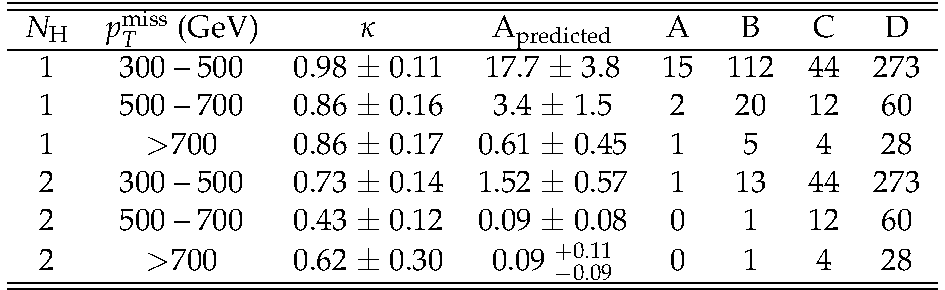
\includegraphics[width=0.75\textwidth]{figs/SUS17006/CMS-SUS-17-006_Table-aux_001.pdf}
\label{tab:sidebandyields}
\end{table}

\input signal-systematics.tex

\section{Yields in the Signal Regions and Exclusion Curves}
\label{sec:results}

After unblinding the 4x3=12 sideband regions and performing the background estimation the 2x3=6 signal regions were unblinded. The observed yields, along with the SM background predictions, are seen in Table \ref{tab:DataPred}. Our signal region yields are consistent with the SM background expectation. Additionally, Table \ref{tab:DataPred} shows the expected signal yields for two model points corresponding to gluino $\tilde{g}$ masses of 2000 or 1800 GeV; the mass of the neutralino $\tilde{\chi}_{1}^{0}$ is fixed at 1 GeV; the mass splitting between the gluino $\tilde{g}$ and neutralino $\tilde{\chi}_{2}^{0}$ is fixed at 50 GeV.

\begin{table}
\caption{Signal yields and SM background predictions}
\centering
\begin{tabular}{c|c|c|c|c||c|c|}
\hline \hline
\ptmiss bin & ABCD Pred & $\kappa$ & Total Pred. & Obs. & T5HH(2000) & T5HZ(1800) \\
\hline \hline
\multicolumn{7}{c}{1-Higgs Tag} \\ \hline \hline
\ptmiss [300,500] & $18.05 \pm 3.39$  & $0.98 \pm 0.11$ & $17.68 \pm 3.85$ & 15 & 0.24 & 0.75  \\ \hline
\ptmiss [500,700] & $4 \pm 1.54$ & $0.86 \pm 0.16$ & $3.44\pm 1.47$ &  2  & 0.32 & 0.98 \\\hline
\ptmiss $>$ 700 &  $0.71 \pm 0.50$  &  $0.86 \pm 0.17$ & $0.61\pm 0.45$ &  1 & 2.13 & 4.34\\\hline \hline
\multicolumn{7}{c}{2-Higgs Tag} \\  \hline \hline
\ptmiss [300,500] &   $2.09 \pm 0.67$  & $0.73 \pm 0.14$ & $1.52 \pm 0.57$ & 1 & 0.17 & 0.35\\ \hline
\ptmiss [500,700] & $ 0.2 \pm 0.20$ & $0.43 \pm 0.12$ &$0.09^{+0.08}_{-0.08}$ & 0 & 0.23 & 0.44\\ \hline
\ptmiss $>$ 700 & $0.14 \pm 0.16$ & $0.62 \pm 0.30$ & $0.09^{+0.11}_{-0.09}$ & 0 & 1.36 & 1.98\\ \hline
\hline
\end{tabular}
\label{tab:DataPred}
\end{table}

A visual representation of the one event in the double-H tagged signal bin is seen in Figure \ref{fig:fireworks}. This event has an additional low-$p_{T}$ AK8 jet. The purple line represents \ptmiss. The yellow cones are the AK8 jets.

\begin{figure}
\centering
\begin{subfigure}[b]{0.49\textwidth}
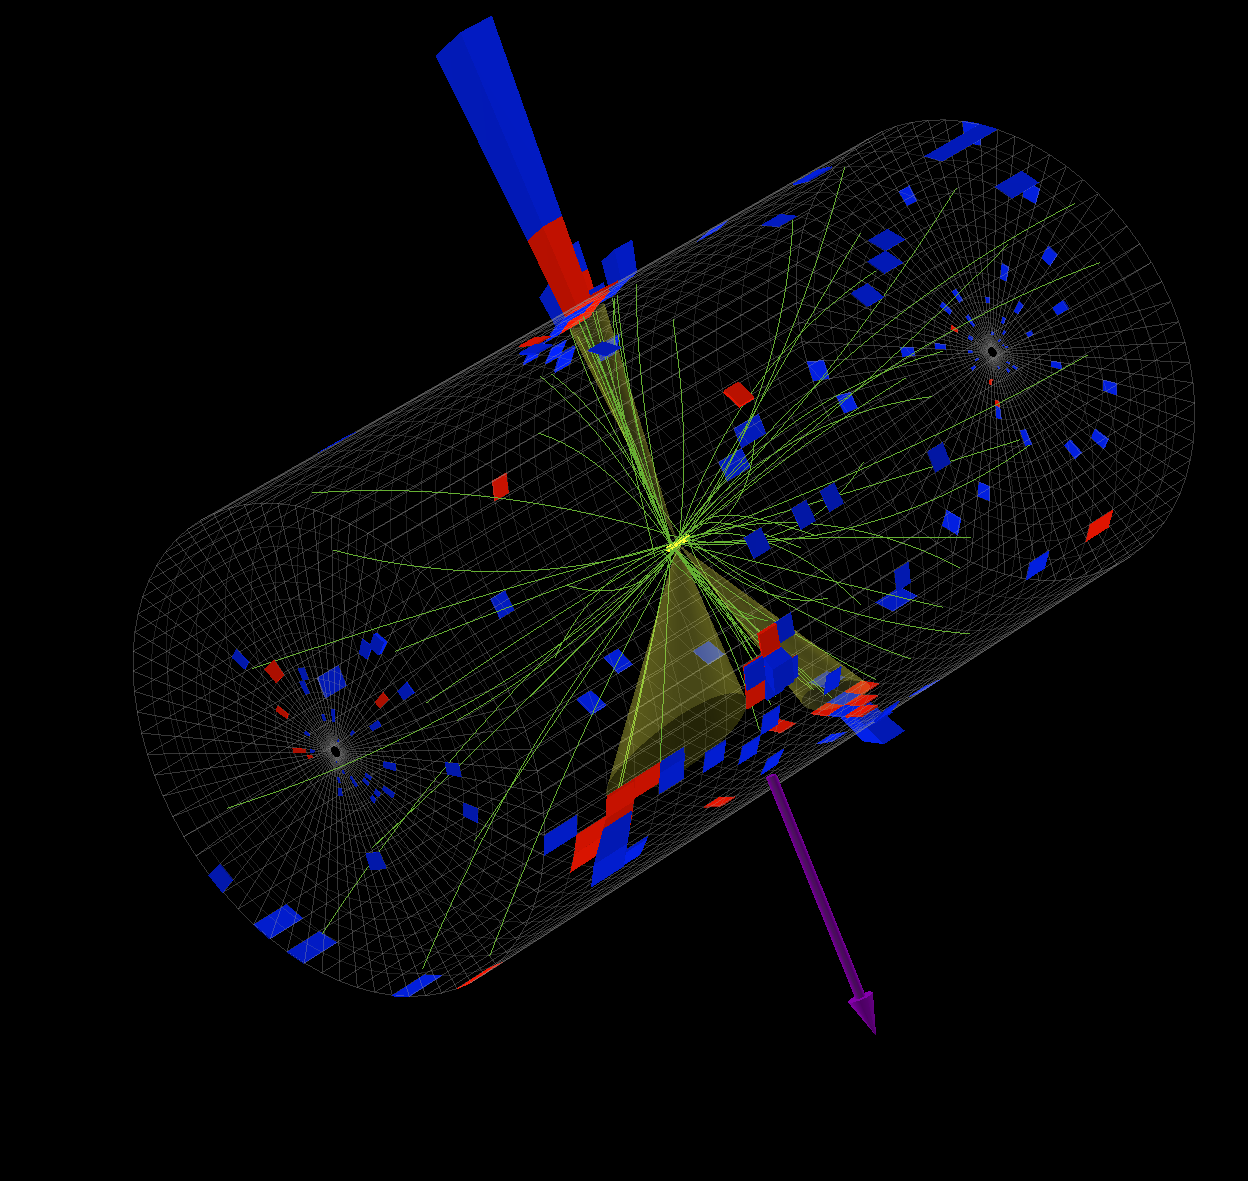
\includegraphics[width=\textwidth]{figs/SUS17006/fireworks_ak8barrel.png}
\end{subfigure}
\begin{subfigure}[b]{0.49\textwidth}
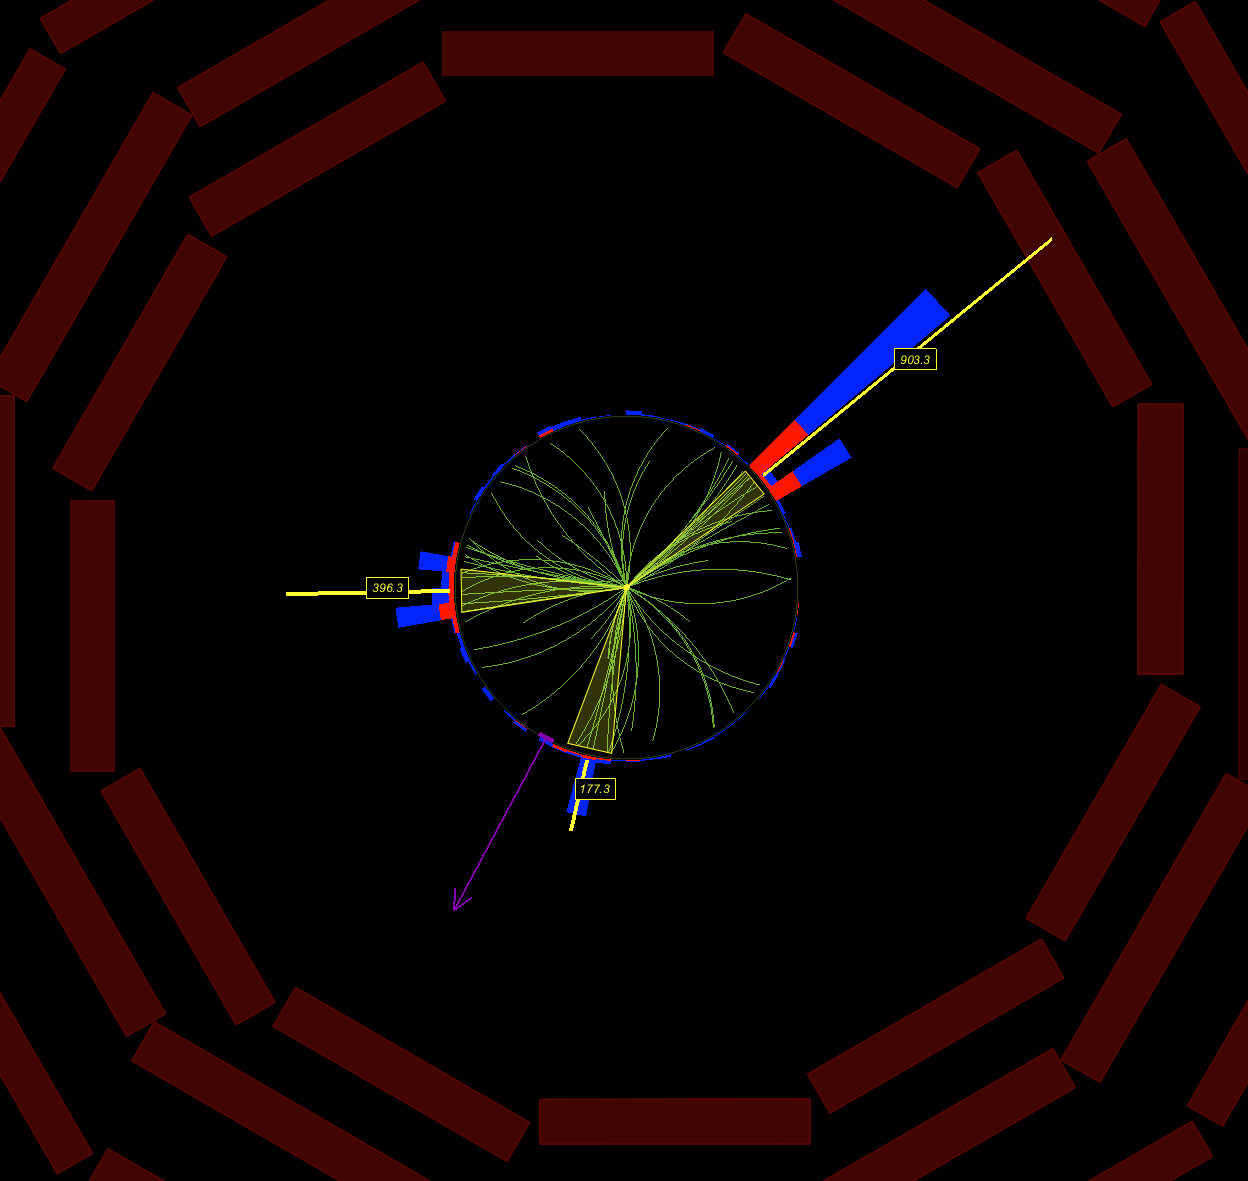
\includegraphics[width=\textwidth]{figs/SUS17006/fireworks_ak8rhophi.png}
\end{subfigure}
\caption{The one event in the double-H tagged signal region.}
\label{fig:fireworks}
\end{figure}

Interpreting our results in the context of the T5HH or T5ZH models, the absence of signal allows us to place lower limits on the mass of the gluino $\tilde{g}$. For the statistical treatment, we use the Higgs combination tool to encode the ABCD approach in the likelihood. In this approach, the data card for one search bin contains the observed number of events and the expected signal and background in each of the ABCD regions. A likelihood function is built that contains these ABCD regions and explicitly encodes the relation $A=\kappa B \frac{C}{D}$ and a Gaussian nuisance is assigned for the uncertainty on $\kappa$. The likelihood for each search bin can be described by:

\begin{equation}
\mathcal{L}=\prod^{ABCD}_{i} Poisson\left(n_i \vert bkg_i + r\cdot sig_i\right) \times \prod^{nuisances}_j Constraints\left(\theta_j , \hat{\theta}_j\right)
\end{equation}

where the 4 regions are modeled by Poisson distribution and the term Constraints refers to either Gaussian distributions for the $\kappa$ uncertainties or log normal distributions that model the signal systematics. The expected and observed limits are then calculated based on the asymptotic approximation of the profile likelihood ratio using the CLs criterion to place limits at the $95\%$ confidence level. These exclusion curves are seen in Figure \ref{fig:brazil}. We are able to place lower limits at 95\% confidence level on the gluino $\tilde{g}$ mass at 2010 and 1825 GeV for the T5HH and T5ZH models, respectively. The weaker limit for the T5ZH model is due to the smaller branching fraction of the Z boson to b-quarks and our choice of signal mass window not being optimal for Z reconstruction.

\begin{figure}
\centering
\begin{subfigure}[b]{0.49\textwidth}
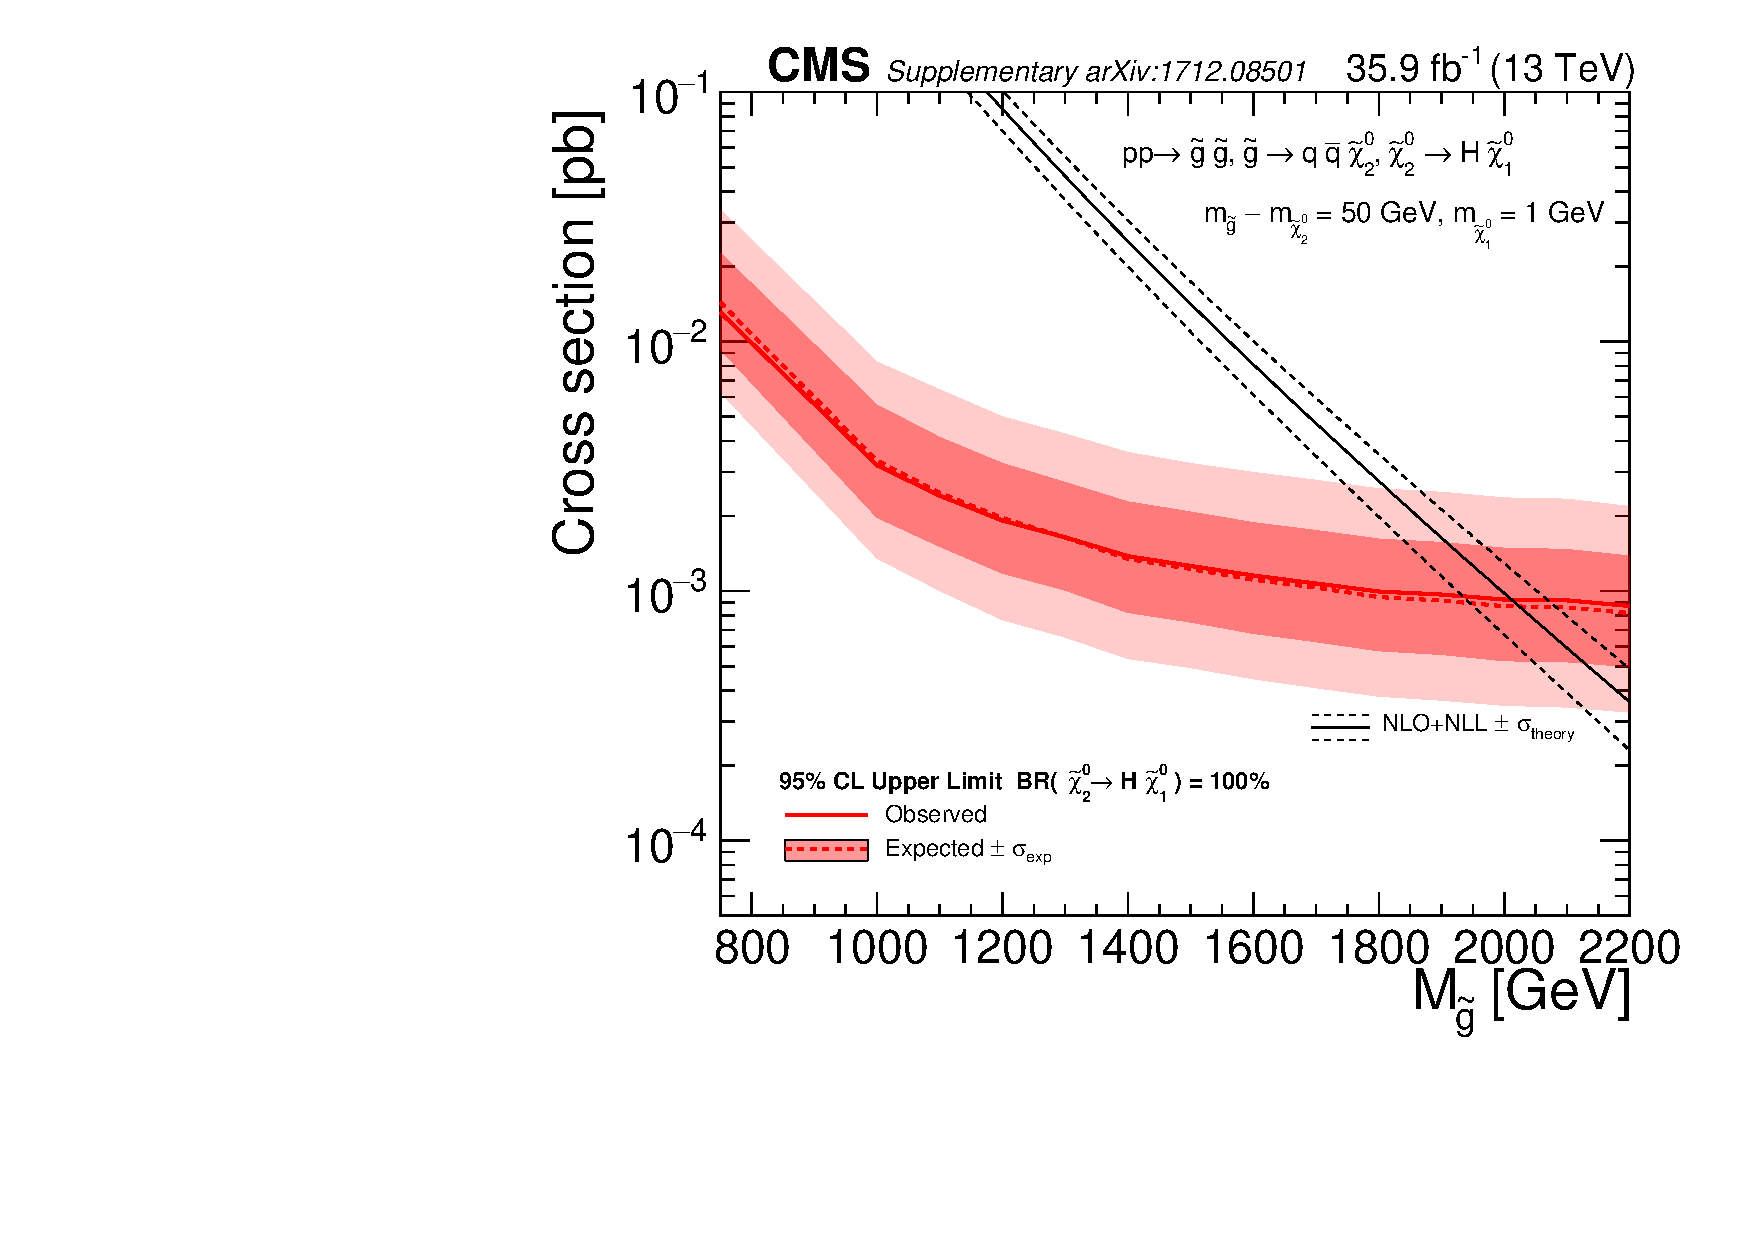
\includegraphics[width=\textwidth]{figs/SUS17006/brazilT5HHResults.pdf}
\caption{T5HH}
\end{subfigure}
\begin{subfigure}[b]{0.49\textwidth}
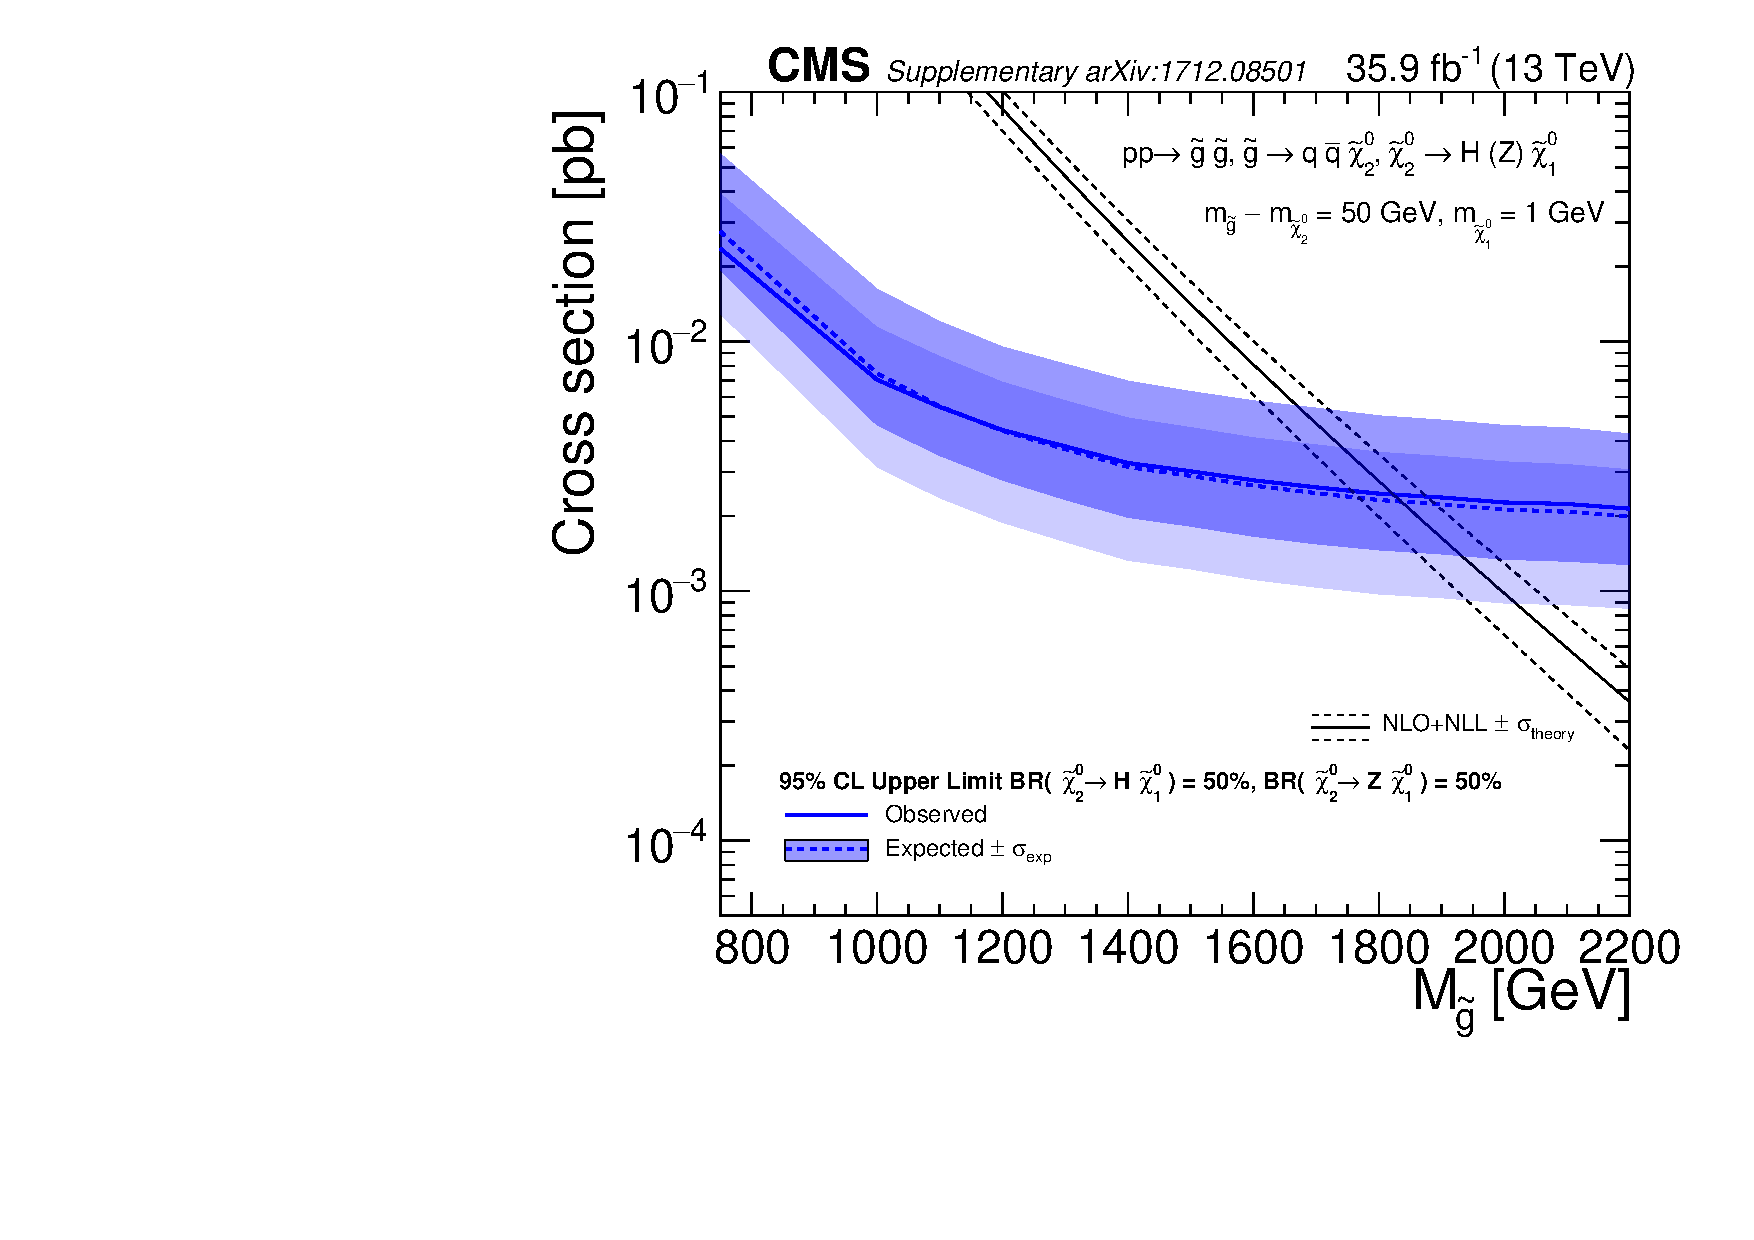
\includegraphics[width=\textwidth]{figs/SUS17006/brazilT5HZResults.pdf}
\caption{T5ZH}
\end{subfigure}
\caption{Observed and expected limits on the gluino cross section.}
\label{fig:brazil}
\end{figure}

\section{Reinterpretation}
\label{sec:reinterpretation}

In Section \ref{sec:results} our results were presented in the context of limit-setting for the T5HH and T5ZH models. Many such SMS models exist within the MSSM which predict the production of high-$p_{T}$ bosons and it is therefore important to include information necessary to make predictions of yields for different final states. This is aided by providing the user with efficiencies for $b\bar{b}$ tagging and mass tagging of the AK8 jets. Tagging efficiencies for the five largest decay channels relevant to the analysis for the H boson are seen in \ref{fig:effH}. Tagging efficiencies for the hadronic decay modes of the Z boson are seen in Figure \ref{fig:effZ}, the much lower mass tagging efficiency for the Z boson is due to our choice of signal mass window [85, 135 GeV] not being optimal for Z boson reconstruction. These are used to calculate the expected yields in the 6 analysis regions when performing a reinterpretation of the analysis using different final states. 

For each event, the yield in each bin can be predicted by first forming the following weights using the tagging efficiencies for the leading two jets, as seen below. j0 and j1 represent the leading and subleading AK8 jet, respectively. The weights on the right-hand-side are $p_{T}$ dependent.

\begin{itemize}
\item double mass tag weight = $j0_{signalmass} \cdot j1_{signalmass}$
\item anti mass tag weight = $(j0_{sidebandmass} \cdot j1_{signalmass}) + (j1_{signalmass} \cdot j1_{sidebandmass}) + (j0_{sidebandmass} \cdot j1_{sidebandmass})$
\item double bb tag weight = $j0_{bbtag} \cdot j1_{bbtag}$
\item single bb tag weight = $(j0_{bbtag} \cdot (1-j1_{bbtag})) + ((1-j0_{bbtag})\cdot j1_{bbtag})$
\item anti bb tag weight = $(1-j0_{bbtag}) \cdot (1-j1_{bbtag}$)
\end{itemize}

These weights are then combined in the following manner to determine the yields across each of the 6 bins for a single event.

\begin{itemize}
\item A1 weight = (single bb tag weight) $\cdot$ (double mass tag weight)
\item A2 weight = (double bb tag weight) s$\cdot$ (double mass tag weight)
\item B1 weight = (single bb tag weight) $\cdot$ (anti mass tag weight)
\item B2 weight = (double bb tag weight) $\cdot$ (anti mass tag weight)
\item C weight = (anti bb tag weight) $\cdot$ (double mass tag weight)
\item D weight = (anti bb tag weight) $\cdot$ (anti mass tag weight)
\end{itemize}

These weights for the 6 analysis bins (inclusive in \ptmiss) are then summed over all events to get the expected yields.
Following this prescription, the authors performed this prediction using the T5HH model with a gluino mass of 2200 GeV and compared to the true value.
The largest deficit was in the D region, with a difference of -36\% difference from nominal.
The greatest over-prediction is found in the B2 region, with a surplus of +8.2\% events relative to nominal.
The closure in the other bins fall somewhere in this range.
These results are summarized in Table \ref{tab:predclos}.
As a further cross-check to the yield estimates, Table \ref{tab:sigeff} shows the true signal event efficiencies for the T5HH model with a gluino mass of 2200 GeV.

\begin{figure}
\begin{centering}
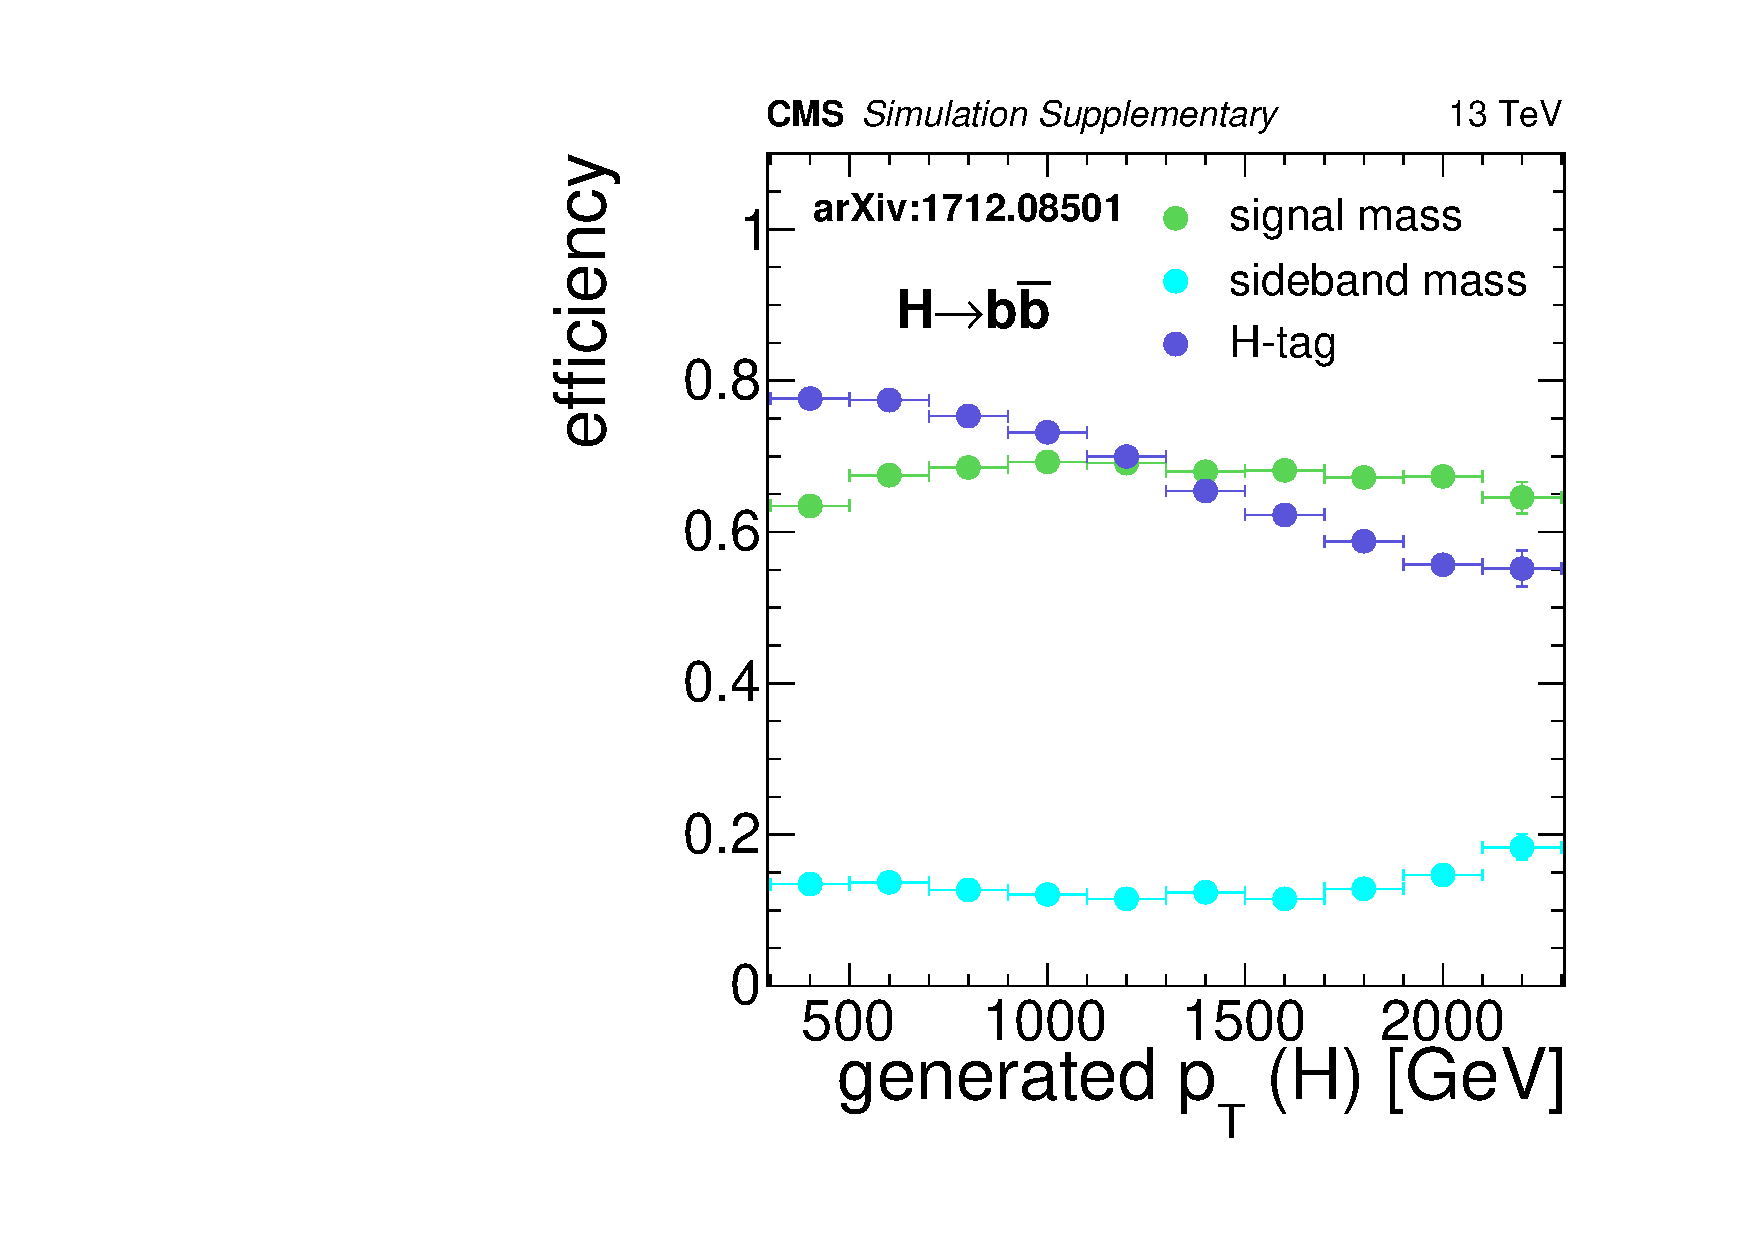
\includegraphics[width=0.45\textwidth]{figs/SUS17006/CMS-SUS-17-006_Figure-aux_006.pdf}
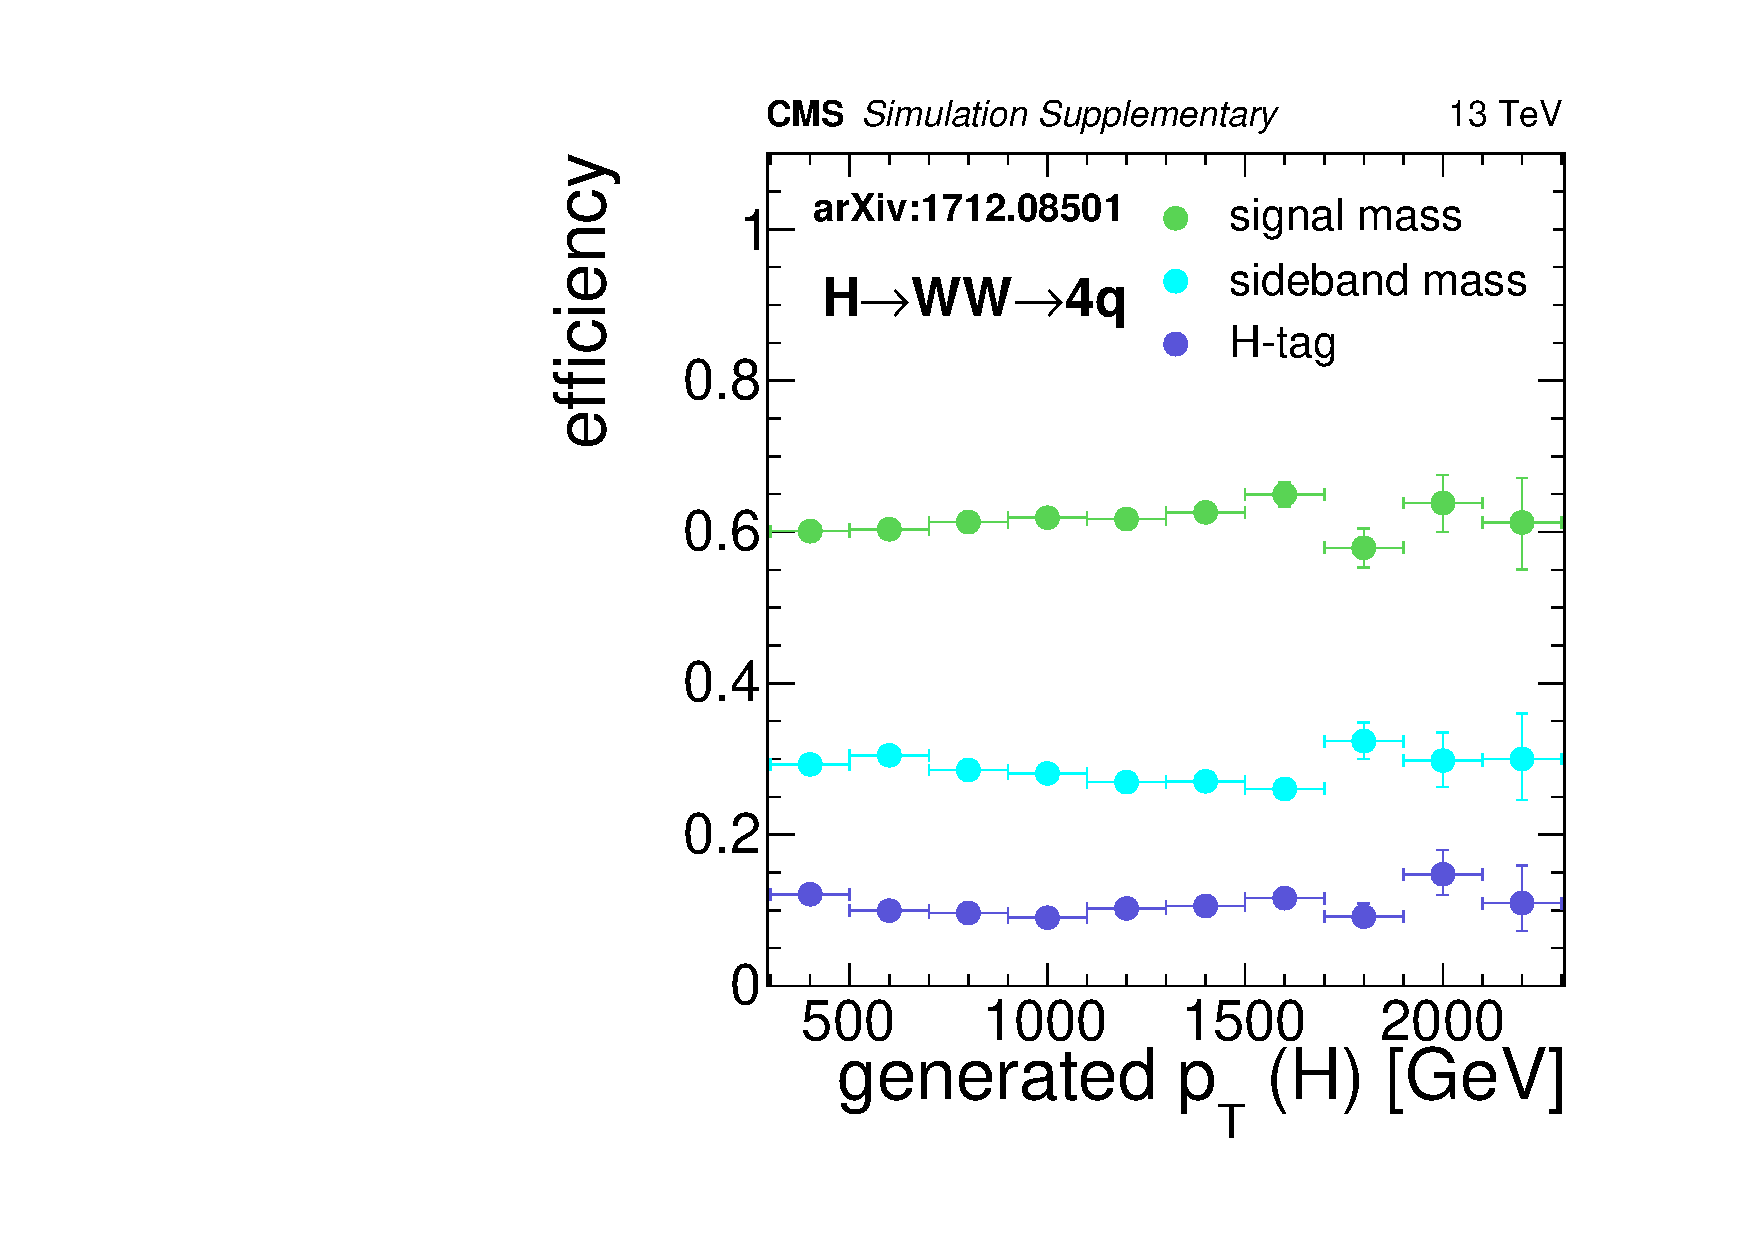
\includegraphics[width=0.45\textwidth]{figs/SUS17006/CMS-SUS-17-006_Figure-aux_007.pdf}
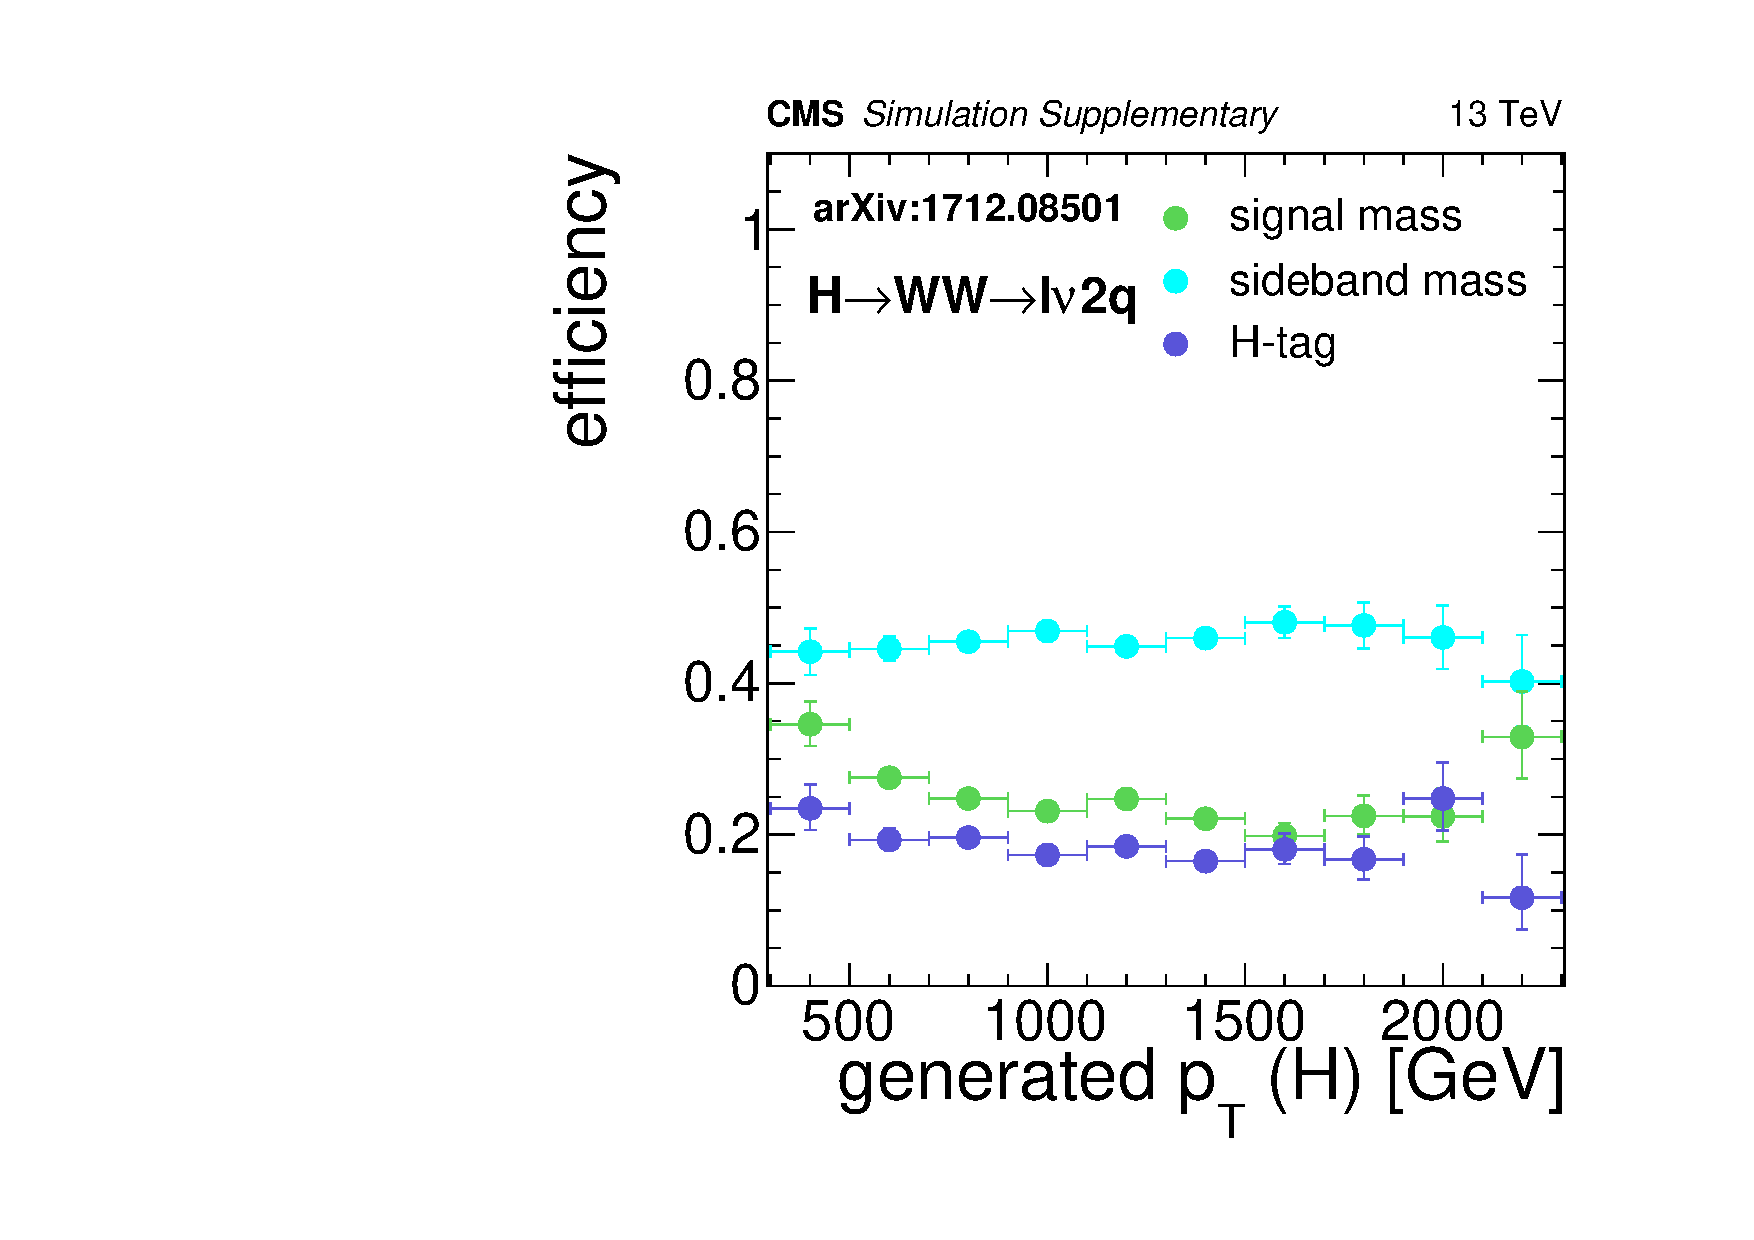
\includegraphics[width=0.45\textwidth]{figs/SUS17006/CMS-SUS-17-006_Figure-aux_008.pdf}
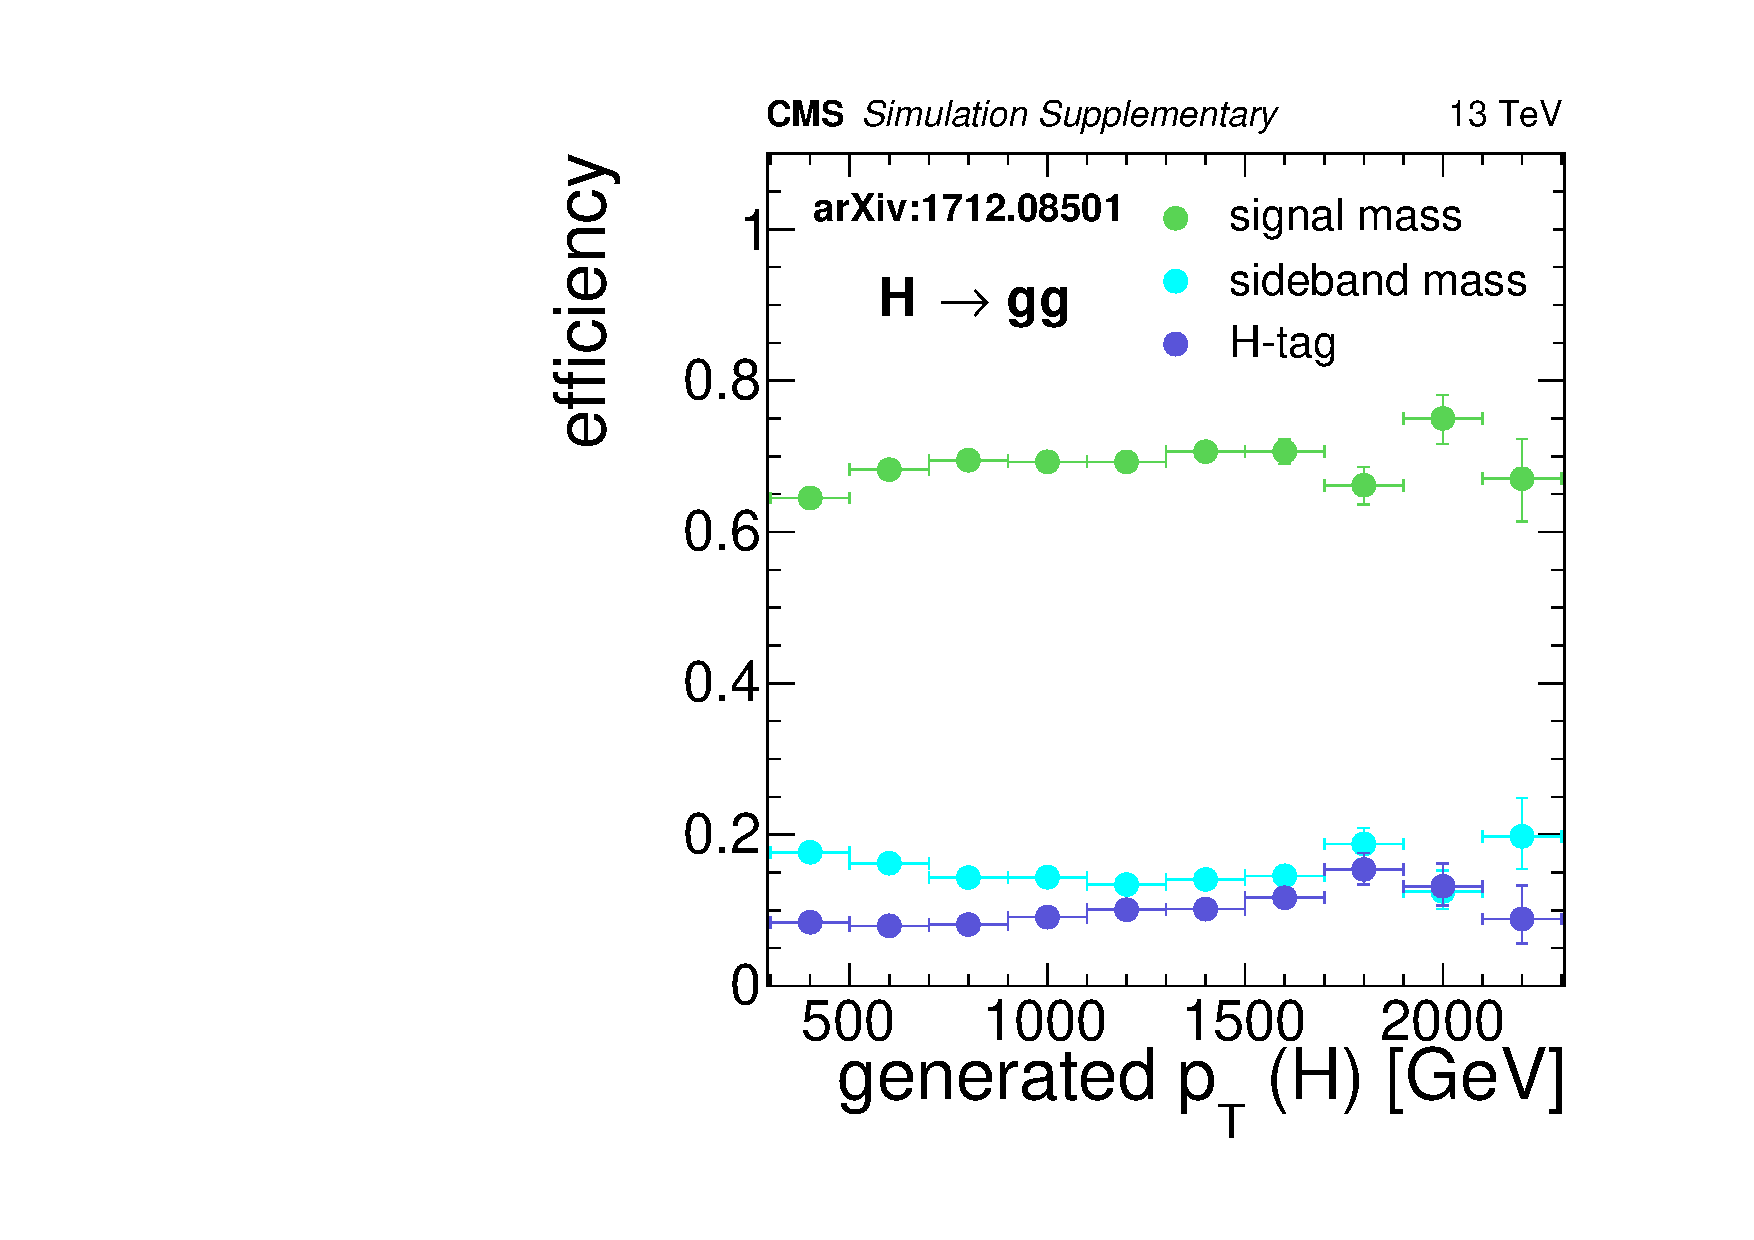
\includegraphics[width=0.45\textwidth]{figs/SUS17006/CMS-SUS-17-006_Figure-aux_009.pdf}
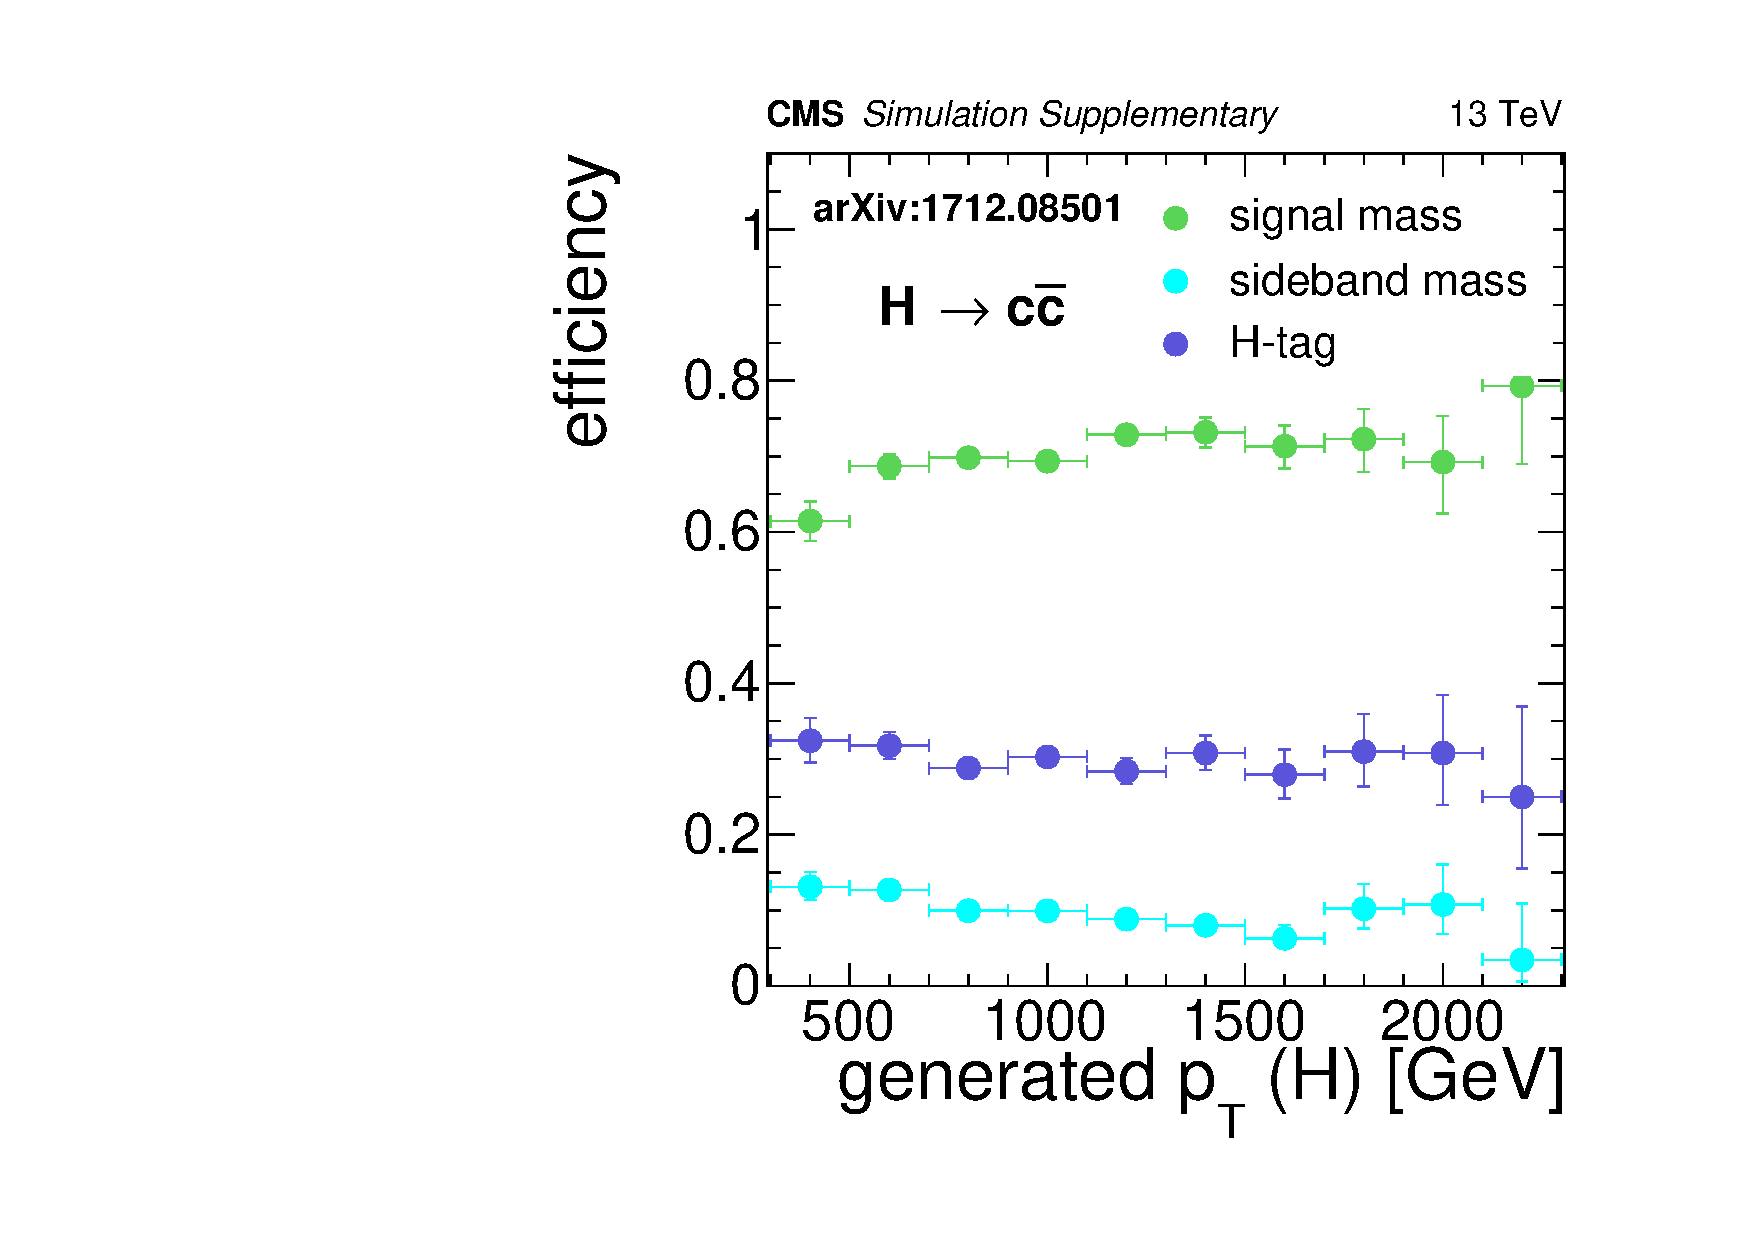
\includegraphics[width=0.45\textwidth]{figs/SUS17006/CMS-SUS-17-006_Figure-aux_010.pdf}
\end{centering}
\caption{
Efficiencies for an AK8 jet originating from Higgs boson decay, relative to baseline selection.
The "signal mass" curve represents the probability the jet will fall within the mass region [85, 135 GeV].
The "sideband mass" curve represents the probability the jet will fall within the mass region [50, 85 GeV] or [135, 250 GeV].
The "H-tag" curve represents the probability the jet have a double-b discriminator value greater than 0.3, for jets within the mass region [50, 250 GeV].
The efficiencies were derived using the T5ZH MC with a gluino mass of 2200 GeV.
}
\label{fig:effH}
\end{figure}

\begin{figure}
\centering
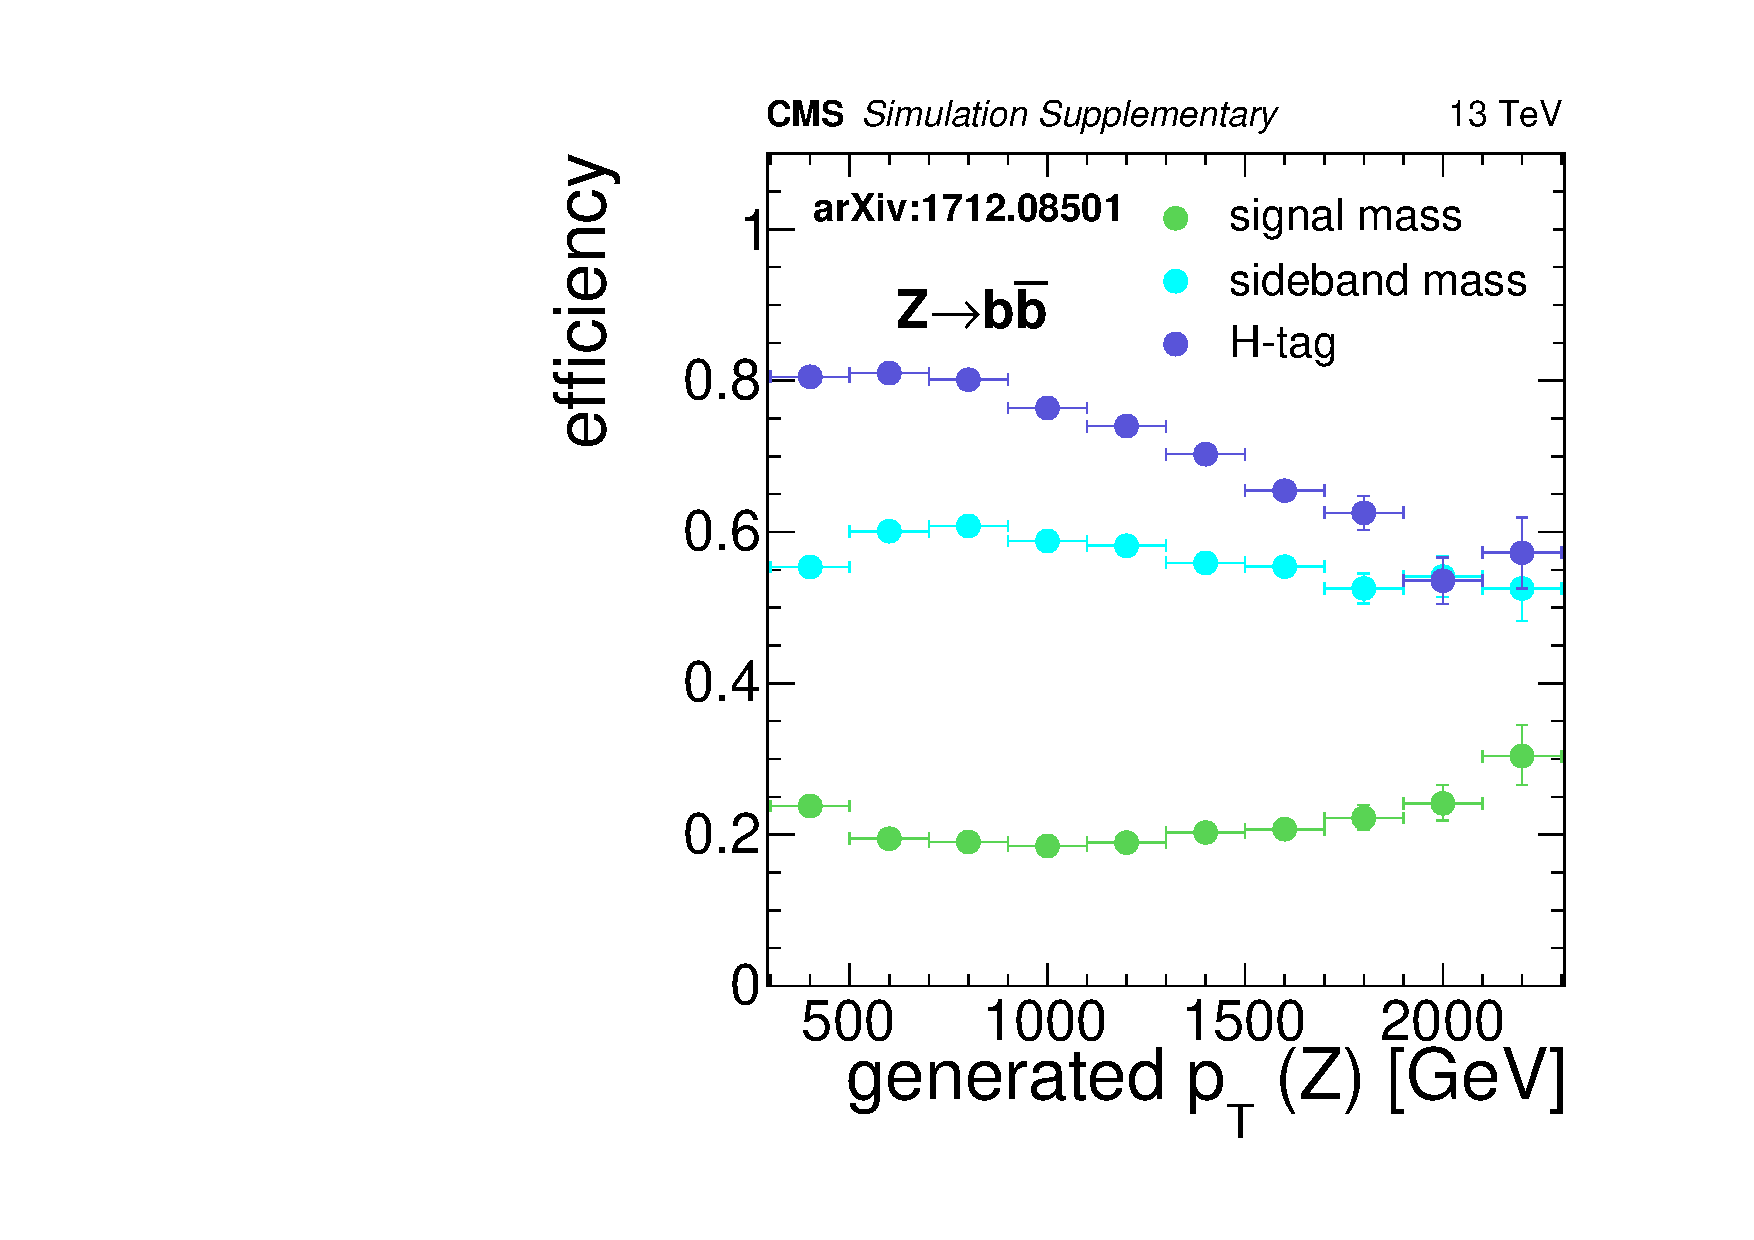
\includegraphics[width=0.45\linewidth]{figs/SUS17006/CMS-SUS-17-006_Figure-aux_011.pdf}
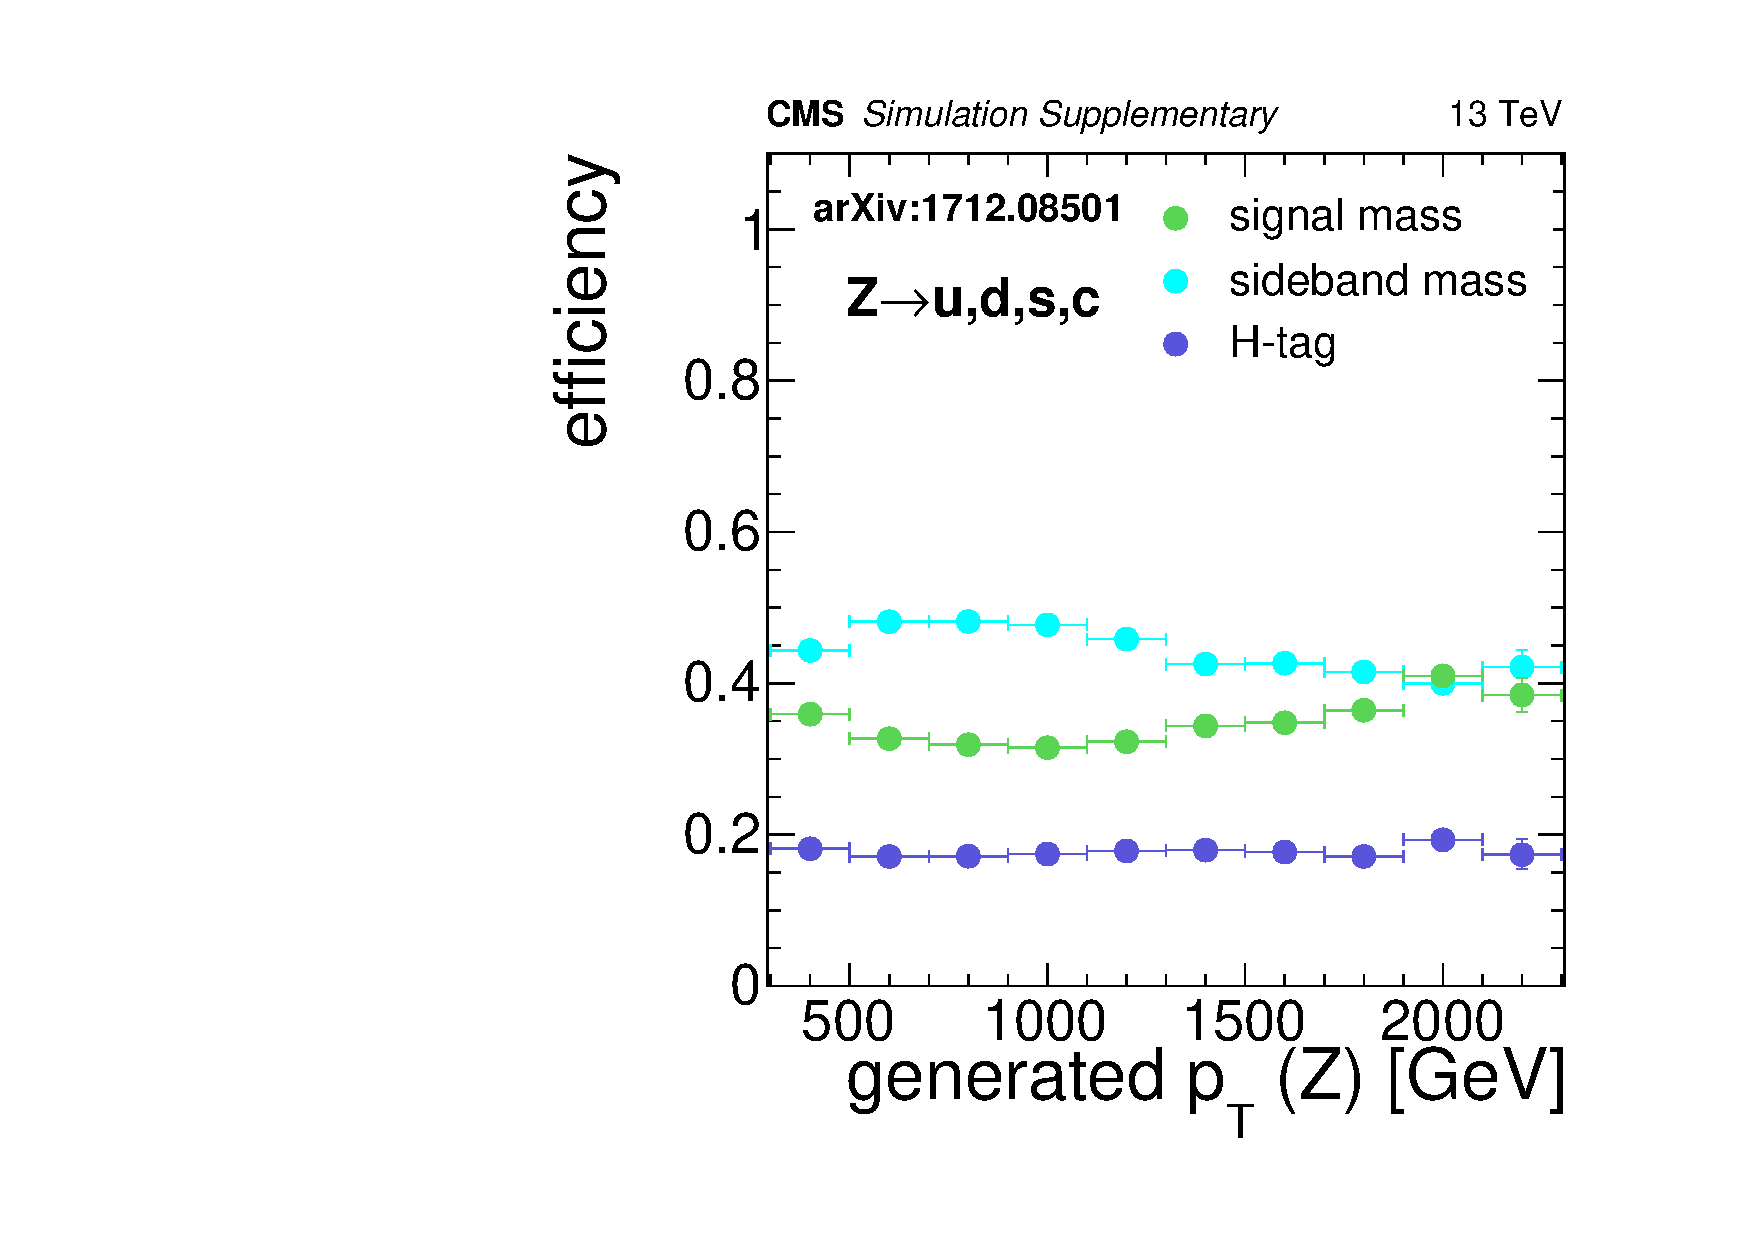
\includegraphics[width=0.45\linewidth]{figs/SUS17006/CMS-SUS-17-006_Figure-aux_012.pdf}\\
\caption{
Efficiencies for an AK8 jet originating from Z boson decay, relative to baseline selection.
The "signal mass" curve represents the probability the jet will fall within the mass region [85, 135 GeV].
The "sideband mass" curve represents the probability the jet will fall within the mass region [50, 85 GeV] or [135, 250 GeV].
The "H-tag" curve represents the probability the jet have a double-b discriminator value greater than 0.3, for jets within the mass region [50, 250 GeV].
The efficiencies were derived using the T5ZH MC with a gluino mass of 2200 GeV.
}
\label{fig:effZ}
\end{figure}

\begin{table}
\centering
\caption{
Comparison of the true reco-level event yield with those obtained via the prediction following the prescription above.
The columns with the RECO or GEN labels are the prediction using RECO or GEN event variables only, respectively.
The prediction was made using the T5HH MC with a gluino mass of 2200 GeV.
}
\begin{tabular}{c | c c c}
\hline\hline
         & RECO     & RECO           & GEN\\
         & "truth"  & prediction     & prediction\\
\hline
Baseline & 4.08     & 3.46 (-15\%)   & 3.53 (-16\%)\\
A1       & 1.21     & 1.18 (-2.3\%)  & 1.26 (+3.6\%)\\
A2       & 0.777    & 0.748 (-3.7\%) & 0.815 (+4.7\%)\\
B1       & 0.802    & 0.703 (-12\%)  & 0.664 (-21\%)\\
B2       & 0.322    & 0.338 (+5.0\%) & 0.350 (+8.2\%)\\
C        & 0.498    & 0.473 (-4.9\%) & 0.487 (-2.1\%)\\
D        & 0.478    & 0.353 (25\%)   & 0.308 (-36\%)\\
\hline\hline
\end{tabular}
\label{tab:predclos}
\end{table}

\begin{table}
\centering
\caption{
Signal efficiencies for an event to land in a given analysis bin.
The efficiencies were derived using the T5HH MC with a gluino mass of 2200 GeV.
Choosing a gluino mass of 1800 GeV decreases the efficiencies by a relative 5\%.
}
\begin{tabular}{c | c c c c c c c c}
\hline
\hline
                                                            & Baseline & A1     & A2      & B1      & B2      & C       & D\\
\hline
$p_{\mathrm{T}}^{\mathrm{miss}}< 300\,\mathrm{GeV}$        & 32\%    & 9.4\%   & 6.0\%   & 6.2\%   & 2.5\%   & 3.9\%   & 3.7\% \\
$300 < p_{\mathrm{T}}^{\mathrm{miss}} < 500\,\mathrm{GeV}$  & 2.7\%   & 0.78\%  & 0.52\%  & 0.54\%  & 0.25\%  & 0.31\%  & 0.30\% \\
$500 < p_{\mathrm{T}}^{\mathrm{miss}} < 700\,\mathrm{GeV}$  & 3.5\%   & 1.0\%   & 0.65\%  & 0.72\%  & 0.28\%  & 0.43\%  & 0.40\% \\
$p_{\mathrm{T}}^{\mathrm{miss}} > 700\,\mathrm{GeV}$        & 26\%    & 7.6\%   & 4.9\%   & 5.0\%   & 2.0\%   & 3.1\%   & 3.0\% \\
\hline
\hline
\end{tabular}
\label{tab:sigeff}
\end{table}

\section{Conclusions}
A search for physics beyond the SM was presented using events with boosted H bosons and missing transverse energy (\ptmiss). The search targeted events with two or more wide-angle jets (AK8) being consistent with the decay of a boosted H or Z boson decaying to \bbbar. \ptmiss could potentially arise in the case a supersymmetric particle escapes detection. An ABCD method uses a sideband region to predict the the SM background in our signal region. Events are categorized according to the \bbbar and mass tagging of the leading two AK8 jets in the event. The observed yields in the 6 signal bins are statistically compatible with the SM background expectation and no excess of events is observed. We use these results to set limits on the gluino mass for the SUSY-inspired T5HH or T5ZH models. For the T5HH model we are able to exclude gluino masses below 2010 GeV at 95\% confidence level. This is with the assumption the NLSP mass is 50 GeV less than the gluino mass and that the LSP has a mass of 1 GeV. The work presented here has been published in a peer-reviewed journal\cite{CMS-SUS-17-006}.
